% vim : foldmethod=marker
\documentclass[a4paper,12pt]{book}

\usepackage{styleperso}
\usepackage{todonotes}

\setuptodonotes{inline, color=blue!30}
% \setlength{\marginparwidth}{2.0cm}
% \bibliography{/home/webersa/Documents/Articles/biblatex.bib}

% =====================================================================================
% ========== Bibliography {{{
\bibliography{/home/samuel/Documents/IGE/Articles/biblatex.bib}
% }}}
% =====================================================================================

% =====================================================================================
% ============= BOOK MARK {{{
% \bookmarksetup{color=blue}
% \bookmark[page=1,level=0]{Sample document}
% }}}
% =====================================================================================

% =====================================================================================
% ========= New command {{{
\DeclareMathOperator*{\argmin}{arg\,min} % thin space, limits underneath in displays
\newcolumntype{P}[1]{>{\centering\arraybackslash}m{#1}}
\renewcommand{\hat}{\widehat}

\newcommand{\E}[1]{\cdot 10^{#1}}
\newcommand{\NOt}{\ce{NO3^-}}
\newcommand{\SOq}{\ce{SO4^2-}}
\newcommand{\NHt}{\ce{NH3}}
\newcommand{\NHq}{\ce{NH4^+}}
\newcommand{\NA}{\ce{NO3NH4}}
\newcommand{\SA}{\ce{SO4(NH4)2}}
\newcommand{\OP}{\text{OP}}
\newcommand{\PM}{\text{PM}}
\newcommand{\PMdix}{\ce{PM10}}
\newcommand{\PMdc}{\ce{PM_{2.5}}}
\newcommand{\PMun}{\ce{PM1}}
\newcommand{\OPm}{\texorpdfstring{\text{OP\textsubscript{m}}}{OPm}}
\newcommand{\OPv}{\texorpdfstring{\text{OP\textsubscript{v}}}{OPv}}
\newcommand{\POm}{\texorpdfstring{\text{PO\textsubscript{m}}}{POm}}
\newcommand{\POv}{\texorpdfstring{\text{PO\textsubscript{v}}}{POv}}
\newcommand{\OPDTT}{\text{OP}$^\text{DTT}$}
\newcommand{\OPDTTv}{\text{OP}$^\text{DTT}_\text{v}$}
\newcommand{\OPDTTm}{\text{OP}$^\text{DTT}_\text{m}$}
\newcommand{\OPAA}{\text{OP}$^\text{AA}$}
\newcommand{\OPAAv}{\text{OP}$^\text{AA}_\text{v}$}
\newcommand{\OPAAm}{\text{OP}$^\text{AA}_\text{m}$}
\newcommand{\PODTT}{\text{PO}$^\text{DTT}$}
\newcommand{\PODTTv}{\text{PO}$^\text{DTT}_\text{v}$}
\newcommand{\PODTTm}{\text{PO}$^\text{DTT}_\text{m}$}
\newcommand{\POAA}{\text{PO}$^\text{AA}$}
\newcommand{\POAAv}{\text{PO}$^\text{AA}_\text{v}$}
\newcommand{\POAAm}{\text{PO}$^\text{AA}_\text{m}$}
\newcommand{\BCwb}{BC\textsubscript{wb}}
\newcommand{\BCff}{BC\textsubscript{ff}}
\newcommand{\Xg}{{\mathbf{X}^{-g}}}
\newcommand{\OMEGA}{\mathbf{\Omega}}

% }}}
% =====================================================================================



\graphicspath{{figures/}}

% =====================================================================================
% ==== Title page {{{
\author{Samuël Weber}
\title{Aerosols sources and their contribution to the oxidative potential of Particulate Matter}
% }}}
% =====================================================================================

\begin{document}


% % \Sethpageshift{26mm}  %%optionnel : à décommenter si besoin pour ajout d'espace afin de center la couvérture horizontalement (valeur par défaut est -5.5mm)
\Sethpageshift{0mm}     %%optionnel : à décommenter si besoin pour ajout d'espace afin de center la couvérture horizontalement (valeur par défaut est -5.5mm)
\Setvpageshift{-17mm}   %%optionnel : à décommenter si besoin pour ajout d'espace afin de center la couvérture verticalement (valeur par défaut est -15.5mm)
%\Universite{}    %%optionnel : à décommenter et à renseigenr si vous voulez changer le non d'université
%\Grade{}         %%optionnel : à décommenter et à renseigenr si vous voulez changer le grade

\Specialite{Océan, Atmosphère, Hydrologie}
\Arrete{25 mai 2016}
\Auteur{Samuël Weber}
\Directeur{Jean-Luc \bsc{Jaffrezo}}
\CoDirecteur{Gaëlle \bsc{Uzu}}    %%optionnel : à décommenter et à renseigenr si présence d'un Co-directeur de thèse
\Laboratoire{Institut des Géosciences de l'Environnement (IGE)}
\EcoleDoctorale{Terre Univers Environnement}
\Titre{Sur les sources du potentiel oxydant des aérosols}
\TitreEN{On the source of the oxydizing potential of aerosols}
% \Soustitre{}      %%optionnel : à décommenter et à renseigenr si présence d'un sous-titre de thèse
\Depot{20 Octobre 2020}
% Commande pour création de nouvelles catégories dans le jury:
%\UGTNewJuryCategory{...NomDeLaCategorie...}{...Definition...}
% Exemple \UGTNewJuryCategory{UGTFamille}{Membre de la famille} que nous ajoutons dans la commande \Jury ci-dessous sous la forme \UGTFamille{Jean Rousseau}{(...titre_et_affiliation...s'il_y_en_a...)}
\Jury{
    \UGTPresident{Didier \bsc{Voisin}}{Professeur, Université Grenoble Alpes -- IGE, Grenoble}
    \UGTRapporteur{Imad \bsc{El Haddad}}{Senior researcher, PSI, Suisse}     %% 1er rapporteur
    \UGTRapporteur{Éric \bsc{Villenave}}{Professeur, Université de Bordeaux -- EPOC, Bordeaux}      %% second rapporteur
    \UGTExaminateur{Matthias \bsc{Beekmann}}{Directeur de recherche, CNRS -- LISA, Paris}   %% 3ème examinateur
    \UGTExaminatrice{Éva \bsc{Léoz-Gardzienda}}{Ingénieure, INERIS, Verneuil-en-hallate}
    \UGTExaminatrice{Nathalie \bsc{Poisson}}{Ingénieure, ADEME, Paris}
    \UGTCoDirectrice{Gaëlle \bsc{Uzu}}{Directrice de recherche, IRD -- IGE}     %% Directeur de thèse
    \UGTCoDirecteur{Jean-Luc \bsc{Jaffrezo}}{Directeur de recherche, CNRS -- IGE}   %% Co-Directeur de thèse s'il y en a
    % \UGTInvite{Cali \bsc{Méro}}{Ingénieur Expert, Laboratoire Pierre Gattaz, Paris} 
}
\MakeUGthesePDG    %% très important pour générer la couverture de thèse

\maketitle

\frontmatter

\clearpage
% \chapter{Acknowledgements}
% \onehalfspacing
% First of all, I wish to thanks Jean-Luc for supporting me during almost
% two years now. Thanks to introduce me to the very interesting topic of Air
% Quality science.  Also, thanks you very much for the confidence you accorded to
% me and for the great opportunities you offer to me in the past two years and
% chaptericularly for the PhD you proposed to me and I accepted cheerfully. 
%
% Thanks also to you, Gaëlle, for successfully supervising my internship from your
% 3600 meter height in La Paz, Bolivia.  Undoubtedly, between Benjamin in Antarctica
% last year and you in Bolivia this year, it seems that one of my supervisor
% always \emph{have to be} in a cold environment, far away from Grenoble :). 
% Thanks for the ideas, your encouragement and your willingness despite the ocean
% and Amazonia between use!
%
% I also wish to thank the little OP-team: Aude and Céline. Thanks for the rich
% discussions we had about OP and error\dots Good luck with the PCA!
%
% Also, many thank to Didier for the frequent \emph{not so silly questions} and
% sharing ideas with you.
%
% Many thanks also to Dalia for sharing your office with me during this internship
% and answering my newbie questions on atmospheric chemistry and also for your
% biscuits at 4 P.M!
%
% And of course, many thanks to Vincent, Coralie and Lisa and all the others for
% the analyses of the sample and dealing with the caprice of the EC/OC or the
% others silly instruments of the lab!
%
% Finally, I am greatful to Jean-Luc (Besombes), not only for his PAH analyses,
% but also for accepting to be my reviewer.
% \normalsize
%

% =====================================================================================
% ====== TableofContent {{{
\tableofcontents
\listoftables
\listoffigures

% }}}
% =====================================================================================

\mainmatter

\chapter*{Introduction}%
\label{cha:introduction}
\addcontentsline{toc}{chapter}{Introduction}
Le rôle d'un travail scientifique est d'observer, d'interroger, de comprendre et d'expliquer. 
Dans ce contexte, la science permet de questionner l'état d'un système, de l'étudier et
éventuellement d'alerter sur ses probables évolutions.

Dans le domaine des sciences du climat ou des géosciences dans leur ensemble, la situation
de changement du climat terrestre a ainsi été observée, comprise et expliquée
par la communauté scientifique, de même que d'autres ``crises'' ou changements brutaux
actuels concernant le système Terre (trou de la couche d'ozone, diminution de la
biodiversité, qualité des eaux et des sols, etc).
Les débats scientifiques ne portent actuellement plus que sur l'affinement des théories et
modèles prédictifs, mais les généralités sont maintenant bien établies et acceptées. C'est
à la société dans son ensemble de trouver une réponse aux dangers auxquels nous faisons
face.

En revanche, l'impact de la qualité de l'air sur les écosystèmes et en particulier sur les
populations humaines est encore mal quantifié. Les observations disponibles sont
parcellaires et la compréhension physico-chimique des processus d'émissions et de
transformations dans l'atmosphère reste à étudier. Aussi, l'impact sur la santé
humaine de la pollution de l'air demande un travail interdisciplinaire important croisant
épidémiologie, toxicologie et géosciences.

La question de l'outil de l'observation de la qualité de l'air est un sujet complexe. La
composition de l'air que nous respirons est extrêmement vaste. Chimiquement, plusieurs
milliers de molécules gazeuses différentes pénètrent dans nos poumons à chaque inspiration.
Physiquement, des particules de tailles variant du nanomètre au centième de millimètre, de
formes et chimies très différentes sont également inspirées et expirées toutes les
secondes par notre organisme. Biologiquement, des pollens, bactéries, spores ou virus
évoluent ou vivent dans l'air que nous respirons.

Ainsi, plusieurs métriques d'observation et de quantification de l'impact sanitaire ont pu
être proposées : distribution en taille des particules, espèces chimiques présentes,
concentration massique.
Mais chacune de ces observations ne regarde qu'un aspect de la pollution. Il est donc
nécessaire de trouver une mesure intégratrice, permettant la prise en compte de la
diversité chimique, physique et biologique de l'air, tout en prenant en compte l'impact
sanitaire potentiel sur le système biologique humain.

L'un des mécanismes suspectés des maladies générées ou accentuées par la pollution de l'air
est imputable à la mise en place d'un état de stress oxydatif dans notre corps, à l'origine des
dysfonctionnements conduisant aux diverses pathologies observées (asthme, maladie
cardiovasculaire, etc). Ainsi, une mesure intégratrice prometteuse concerne la capacité de
l'air inspiré à déséquilibrer nos défenses anti-oxydantes, notamment pulmonaires.
La mesure de cette capacité oxydante de l'air, appelée potentiel oxydant, pourrait être
l'une de ces métriques recherchées.

Cette thèse s'inscrit dans cette démarche de recherches des déterminants de ce potentiel
oxydant des particules atmosphériques. Seulement, pour estimer les sources de potentiel
oxydant, il est nécessaire de se poser en amont la question des sources de particules
atmosphériques. L'utilisation de nombreuses mesures de terrain, collectées et analysées
lors de différents programmes de recherches antérieurs ou actuels, permettra dans un
premier temps la compréhension de différents processus d'émissions et le renforcement de
méthodologies de quantification des sources d'émissions. L'évaluation à grande échelle
spatiale de la contribution des différentes sources d'émission ainsi que leur apport au
potentiel oxydant sera traité dans un second temps. Finalement, quelques pistes de
travaux futurs seront explorés, toujours avec pour objectif principal la mise en place
d'un meilleur indicateur de la qualité de l'air d'intérêt sanitaire.




\chapter{État de l'art}
\label{cha:etat_de_lart}
\PartialToc
\clearpage

\section{Rappel sur la géodynamique de l'atmosphère terrestre}%
\label{sec:structure_atmosphere}

\subsection{Composition chimique de l'atmosphère}%
\label{ssub:composition_chimique_de_latmosphere}

L'atmosphère de la Terre est composée principalement de gaz. Sa composition sèche est
faite de diazote \ce{N2} à \SI{78.087}{\percent}, de dioxygène \ce{O2} à
\SI{20.95}{\percent} et d'argon \ce{Ar} à \SI{0.93}{\percent}. Parmi les pourcentages restant
se trouvent le dioxyde de carbone \ce{CO2} (\SI{0.041}{\percent}) et le méthane \ce{CH4},
en augmentation depuis le début de l'ère industrielle, ainsi que d'autres gaz à
l'état de trace (néon \ce{Ne}, hélium \ce{He} et krypton \ce{Kr}).  Cette composition est
dite ``sèche'' car ne prend pas en compte la vapeur d'eau, représentant en moyenne 
\SI{0.25}{\percent} de la masse totale de l'atmosphère, mais en quantité extrêmement
variable selon l'espace ou le temps.

De plus, sous l'effet des radiations solaires et notamment les longueurs d'ondes
ultra-violettes (UV), de nombreux radicaux, dont les radicaux hydroxyles \ce{HO^.} sont
formés et réagissent rapidement avec les autres composants de l'atmosphère.  La quantité
de dioxygène et la présence de radicaux hydroxyles, entre autres, font de l'atmosphère un
milieu à grande capacité oxydante ayant un impact direct sur les différentes réactions
pouvant avoir lieu, aussi bien avec les gaz à effet de serre qu'avec les polluants, en
particulier organiques, présents dans les basses couches de l'atmosphère.

Enfin, il est à noter que l'atmosphère n'est pas composée que de gaz mais également de
particules solides ou liquides en suspension, que ce soit des cristaux de glace ou de l'eau
liquide sous forme de nuage, mais également des ``poussières'', dont il sera question dans
cette thèse, et qui seront plus explicitement présentées ci-après
section~\ref{sec:les_aerosols_atmospheriques}.

\subsection{Structuration de l'atmosphère}%
\label{sub:structuration_de_l_atmosphere}

\subsubsection{Une organisation stratifiée}%
\label{ssub:une_organisation_stratifiée}

À première vue, l'atmosphère terrestre peut sembler homogène depuis le sol jusqu'à
l'espace. En réalité, de grandes hétérogénéités sont observées à certaines altitudes,
formant des couches concentriques aux propriétés physico-chimiques très différentes, ne se
mélangeant que peu, limitant ainsi les échanges entre elles (voir
Figure~\ref{fig:chapter01/Comparison_US_standard_atmosphere_1962}).

Notamment, c'est dans la première strate atmosphérique, de \SI{0}{km} à \SI{13}{km} en
moyenne, la troposphère, que se déroulent les phénomènes météorologiques
``directement sensibles'' au quotidien
(convection, formation de nuages, transport longue distance de poussières…).
C'est aussi la troposphère qui totalise près de \SI{75}{\percent} de la masse totale
de l'atmosphère et contient la quasi-totalité de l'eau et des aérosols, ce qui nous
intéresse particulièrement pour cette thèse.

La tropopause marque la séparation entre la troposphère et la stratosphère. Elle est
notable par son changement brutal de gradient thermique (\SI{-6}{\degreeCelsius\per\km}
dans la troposphère, à \SI{0}{\degreeCelsius\per\km} dans le bas de la stratosphère).
Ceci conduit à une inversion thermique très forte, faisant de la tropopause une véritable
barrière physique. La présence de la couche d'ozone (\ce{O3}) dans la stratosphère
protège la surface de la Terre d'une partie des UV provenant du Soleil, en absorbant ses
radiations. Du fait de cette absorption par l'ozone, la stratosphère se réchauffe
progressivement avec l'altitude, jusqu'à arriver à une nouvelle frontière : la
stratopause, marquée par un gradient thermique proche de 0.

Vient ensuite la mésosphère, dénuée d'ozone et peu concentrée en autres gaz et présentant
donc un refroidissement du fait de la faible absorption du rayonnement solaire. Puis la
dernière strate, la thermosphère, est réchauffée sous l'effet des radiations solaires
formant des ions par photodissociation.
C'est également à cette altitude que se produisent les aurores boréales, lorsque les
particules du vent solaire se heurtent au champ électromagnétique terrestre à environ
\SI{100}{km} d'altitude. Finalement, vient l'espace extra-terrestre au-delà \SI{600}{km}
d'altitude.

\begin{figure}[ht]
    \centering
    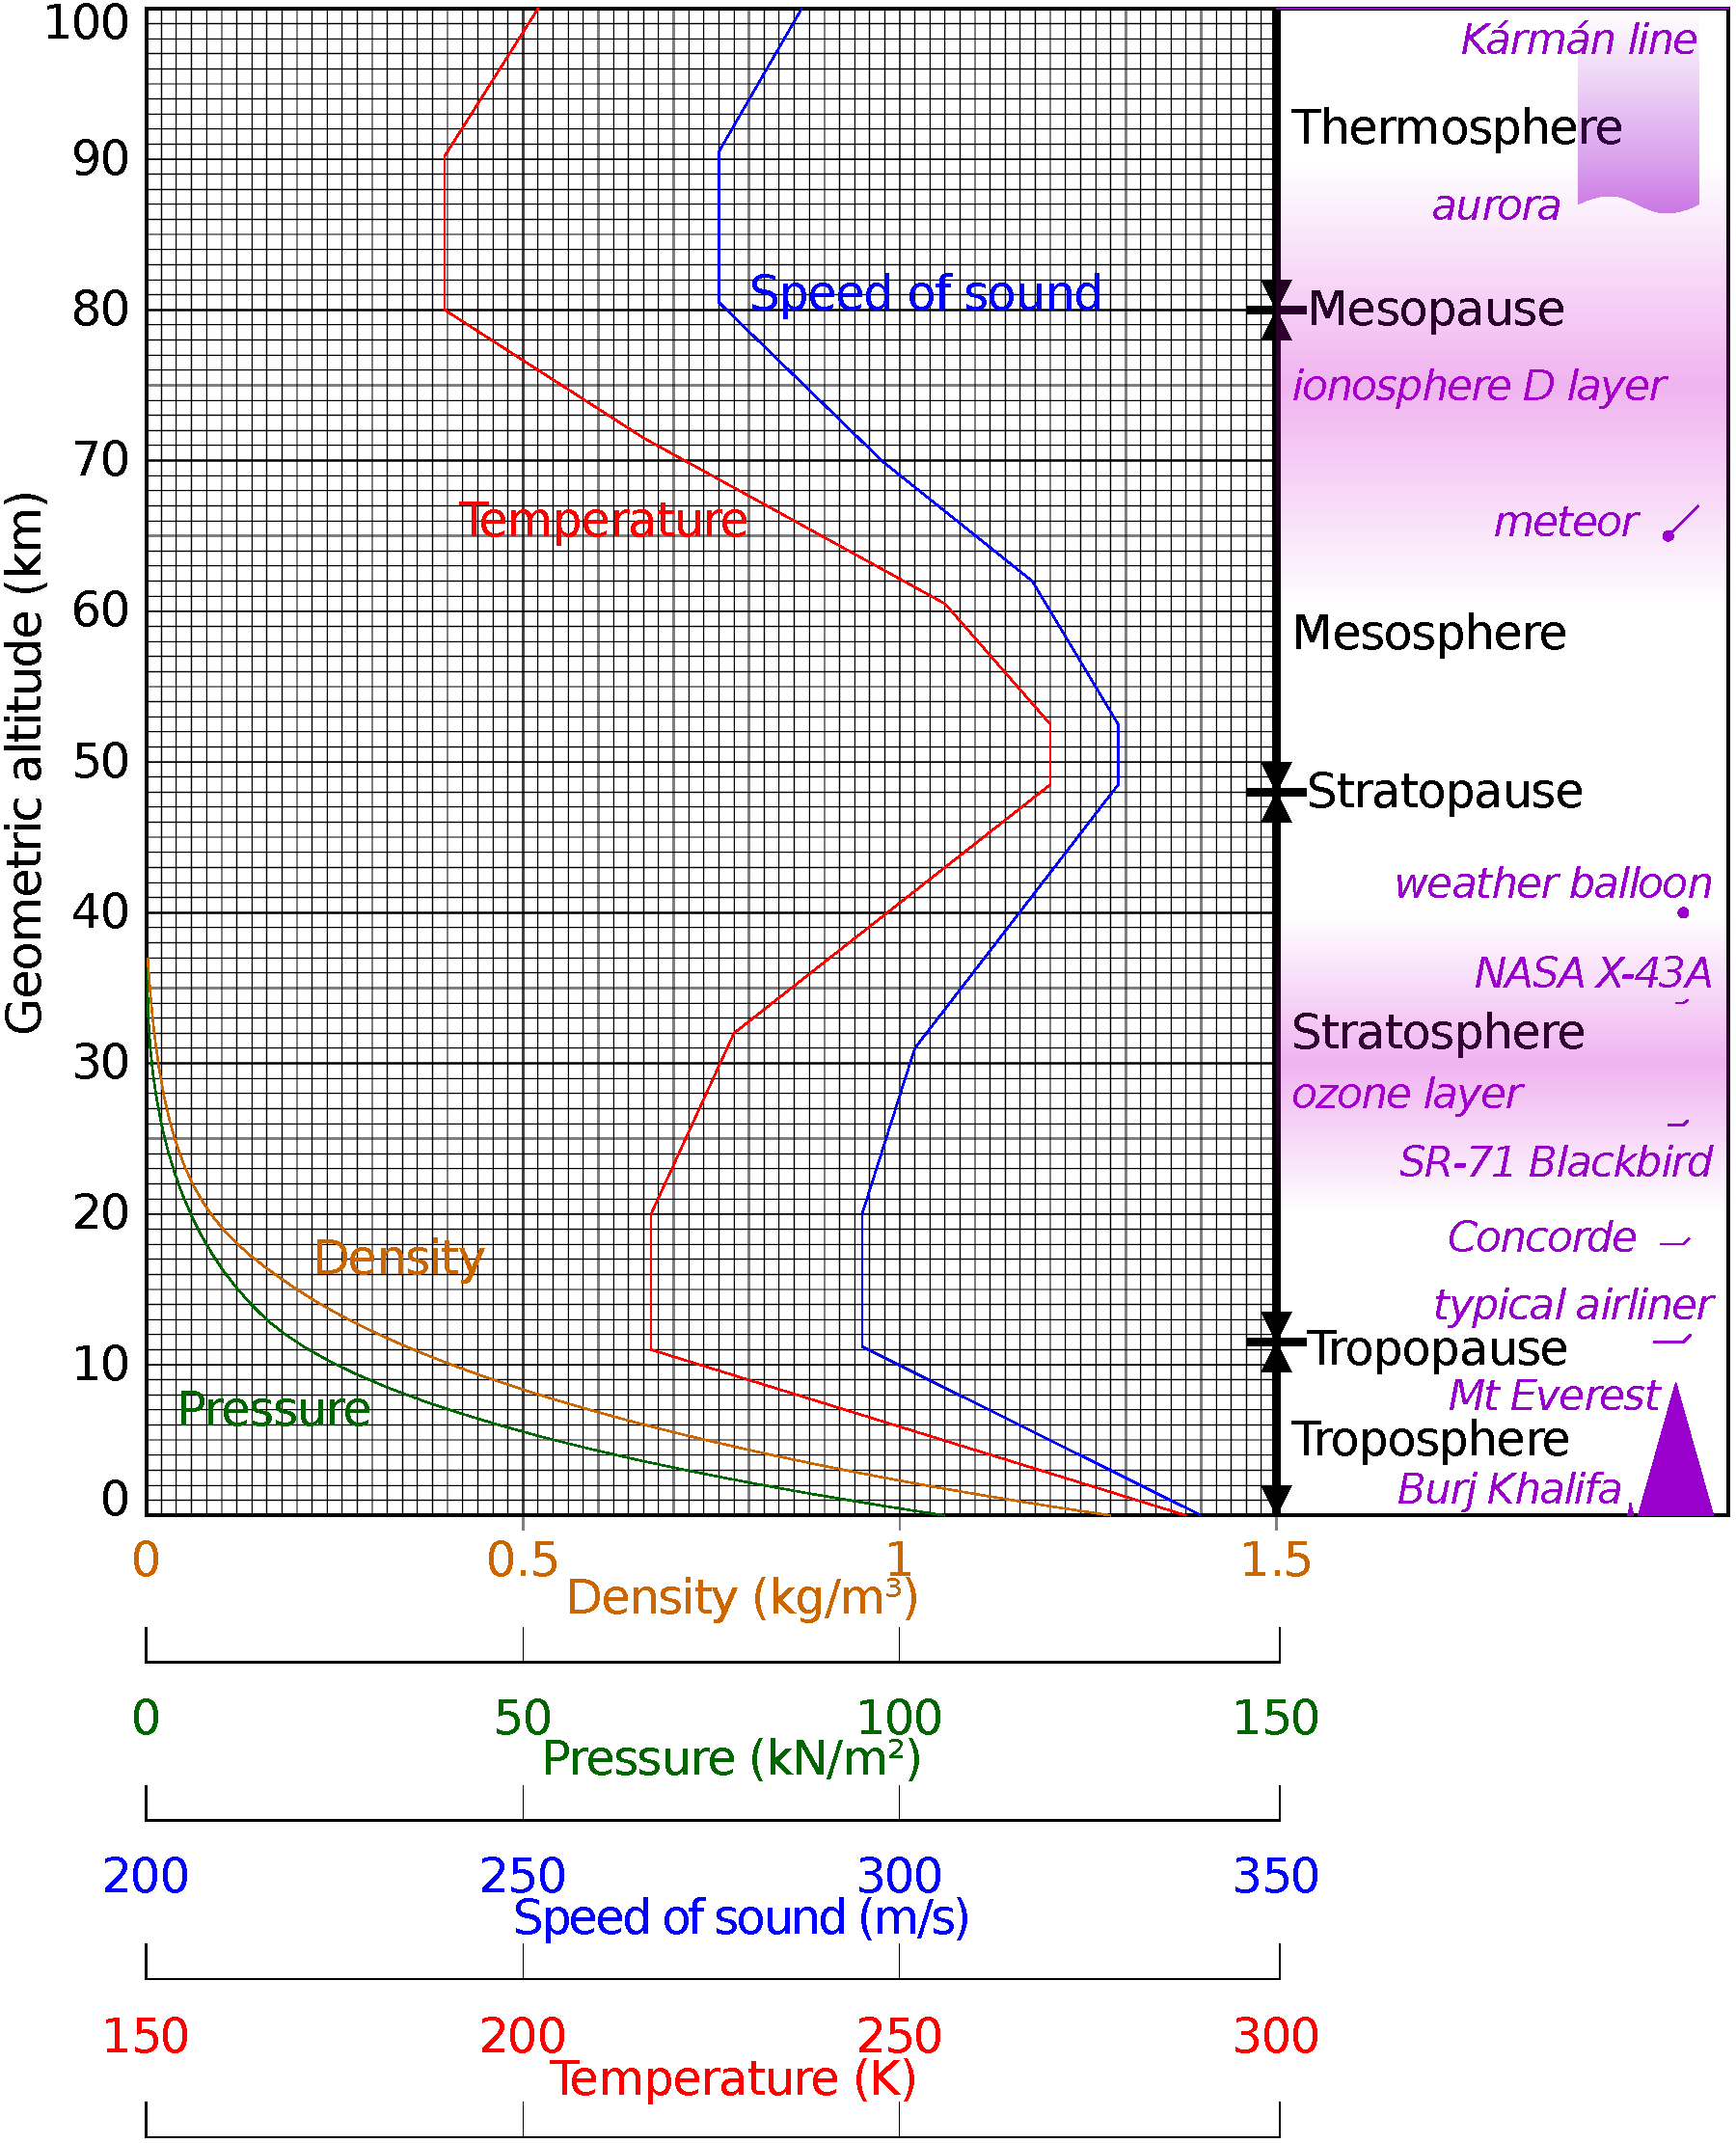
\includegraphics[width=0.6\linewidth]{chapter01/Comparison_US_standard_atmosphere_1962.pdf}
    \caption{%
        Comparaison des variables atmosphériques selon l'atmosphère standard définie par
        l'\textit{US standard atmosphere} de 1962.
        Source:
        \href{https://commons.wikimedia.org/wiki/File:Comparison_US_standard_atmosphere_1962.svg}{wikicommons},
        par \href{https://commons.wikimedia.org/wiki/User:Cmglee}{Cmglee}, CC-BY-SA.
    }%
    \label{fig:chapter01/Comparison_US_standard_atmosphere_1962}
\end{figure}

\subsubsection{La couche limite atmosphérique}%
\label{sub:la_couche_limite_atmospherique}

À l'intérieur de cette fine couche d'environ \SI{600}{km}, seule la troposphère,
c'est-à-dire les 13 premiers kilomètres, nous est directement familière. C'est en effet
dans la troposphère que les phénomènes météorologiques auxquels nous sommes habitués s'y
déroulent : nuage, vent, pluie, etc. Alors que l'atmosphère paraît immense, il est
important de noter la faible hauteur de cette couche.

La partie de la troposphère directement impactée par les effets de la surface terrestre
(friction, réchauffement, turbulence) est appelée la couche limite atmosphérique (CLA, ou
\textit{atmospheric boundary layer (ABL))}. Cette couche variant de quelques dizaines à centaines
de mètres selon les lieux et périodes de la journée, a une dynamique rapide et
convective. Notamment intéressant pour cette thèse, cela a pour conséquences que les
émissions de surface anthropiques ou naturelles, et notamment les polluants, sont
redistribuées sur l'intégralité de cette hauteur.

Durant la nuit, la hauteur de la CLA est faible du fait de l'affaiblissement du
gradient thermique vertical lié à l'absence de réchauffement radiatif du sol (voir
Figure~\ref{fig:chapter01/Atmospheric_boundary_layer}) et la mise en place de la couche de
surface après le coucher du soleil. À l'aube, la surface se réchauffe et la
convection se met en place, rendant la CLA beaucoup plus homogène et diluant gaz et
particules dans un plus gros volume d'air. Les composés ne traversent cependant que
rarement la couche d'inversion thermique, limite entre la CLA et la troposphère libre.
Ainsi, après le coucher du soleil, on observe fréquemment une couche résiduelle au milieu de
la CLA qui ``capture'' les composés d'une journée à une autre.

Il est à noter que des couches d'inversions thermiques à plus basse altitude peuvent se
mettre en place, notamment dans les vallées alpines. Pour un flux d'émission
constant, cela entraîne donc une accumulation forte des composés chimiques dans un volume
très restreint, augmentant mécaniquement les concentrations.
\cite{allardQualite2018} a ainsi pu montrer que le gradient thermique est l'un des
facteurs explicatifs le plus important pour la compréhension des concentrations en
vallées alpines.
%Notamment, certains jours à Passy, France, un facteur de concentration de 700 était présent entre 

\begin{figure}[h]
    \centering
    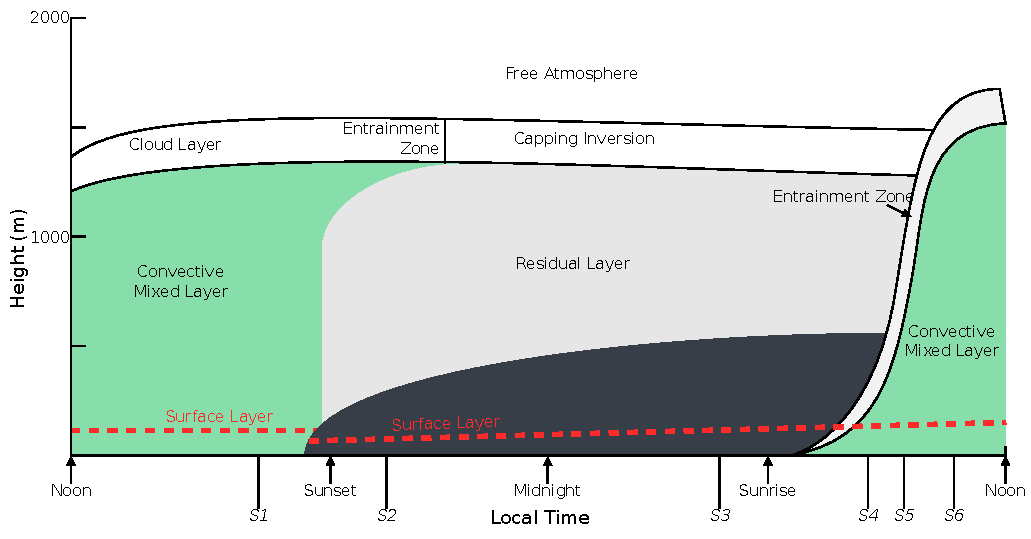
\includegraphics[width=0.8\linewidth]{chapter01/Atmospheric_boundary_layer.pdf}
    \caption{Évolution journalière schématique de la couche limite atmosphérique.
        Credit: By
        \href{https://commons.wikimedia.org/w/index.php?curid=18862904}{NikNaks} - Own
        work based on:
        \url{http://ars.sciencedirect.com/content/image/1-s2.0-S0360128504000371-gr4.jpg}.
        See also: \url{http://www.archaeocosmology.org/eng/tropospherelayers.htm}., CC
        BY-SA 3.0
    }%
    \label{fig:chapter01/Atmospheric_boundary_layer}
\end{figure}


\section{Les aérosols atmosphériques}%
\label{sec:les_aerosols_atmospheriques}

\subsection{Qu'est-ce qu'un aérosol?}%
\label{sub:quest-ce-quun-aerosol}

L'air que nous respirons est constitué majoritairement de gaz (\ce{N2}, \ce{O2}…) mais
également de particules solides ou liquides en suspension dans l'air. Très
légères et de tailles de l'ordre du nanomètre à quelques dizaines de micromètres,
ces particules sont communément appelées particules fines, ou \textit{particulate matter} (PM).

À titre de comparaison, cela reviendrait à grouper dans une même catégorie une marche de
\SI{100}{m} pour aller chercher son pain à un voyage de \SI{10000}{km}.
Ainsi, cette nomenclature ``PM'' regroupe nécessairement des objets aux caractéristiques
très diverses, comme le montre la Figure~\ref{fig:aerosolDistribution}. Selon
que l'on observe les PM en s'intéressant à leur nombre, surface ou volume, l'importance
relative des classes de taille change complètement.

\begin{figure}[ht]
    \centering
    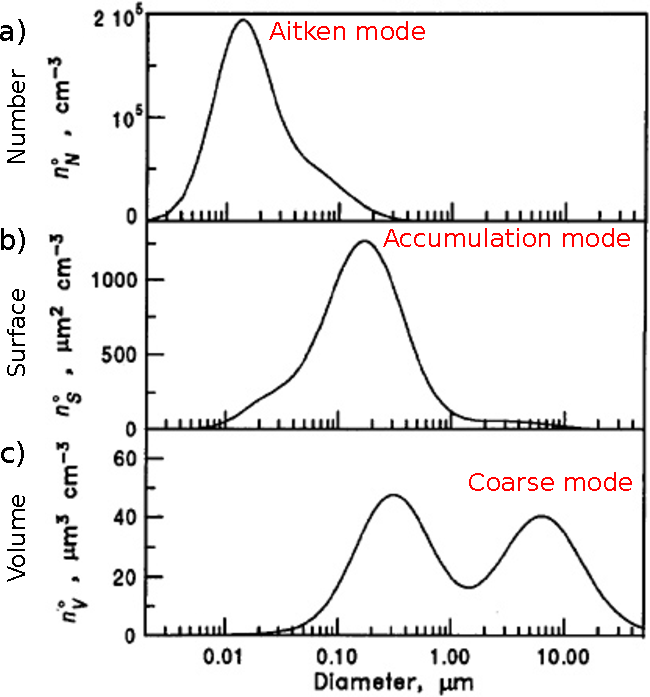
\includegraphics[width=0.5\textwidth]{aerosolDistribution.pdf}
    \caption{Distribution \textbf{(a)} en nombre, \textbf{(b)} surface, et
        \textbf{(c)} volume, pour un ensemble typique de distribution trimodale
        d'aérosols. Figure adaptée du livre de~\cite{seinfieldAtmospheric1998}.}
    \label{fig:aerosolDistribution}
\end{figure}

Ces différentes classes de taille (appelées modes) sont dues à différents procédés à
l'origine de leurs présences dans l'air. Le mode le plus fin et prépondérant en nombre,
dit d'Aikten, correspond à la nucléation à partir de composés gazeux ou de sources de
combustion.  Par coagulations successives et transformations dans les nuages, des
particules plus grosses se forment (mode d'accumulation).  Enfin se forme le mode grossier
alimenté par diverses autres sources comme la remise en suspension de poussières ou sable
par le vent, les pollens, les activités humaines, parmi d'autres, comme nous le verrons
plus loin.

La nomenclature des aérosols est ainsi historiquement fondée sur leur taille:
\begin{itemize}
    \item \PMdix, dont le diamètre aérodynamique est inférieur ou égal à \SI{10}{\um} (petit
        grain de sable, pollens…)
    \item \PMdc, dont le diamètre aérodynamique est inférieur ou égal à \SI{2.5}{\um}
        (suie, fumée…)
    \item \PMun, parfois appelé particules ultrafines (UFP), dont le diamètre
        aérodynamique est inférieur ou égal à \SI{1}{\um} (coagulation et condensation de
        vapeur…)
\end{itemize}


Ces catégories très diverses présentent ainsi des formes variées, comme illustré par les
clichés de microscopies électroniques présentés figure~\ref{fig:micrography}. On retrouve
des particules sphériques de petites tailles, des formes plus géométriques issues de
processus de cristallisation comme le sel marin, etc.

\begin{figure}[ht]
    \centering
    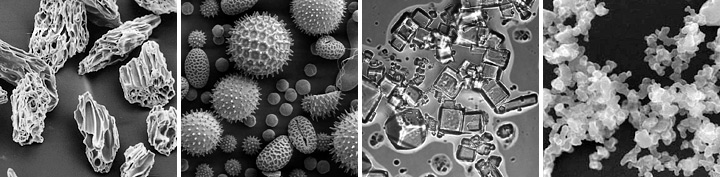
\includegraphics[width=1.0\textwidth]{aerosol_micrographs.jpg}
    \caption{Image au microscope électronique à balayage, à des échelles différentes,
        illustrant la diversité de forme des aérosols.
        De gauche à droite : cendre volcanique, pollen, sel de mer et suie. Micrographies de
        l'USGS, UMBC (Chere Petty) et de l'Arizona State University (Peter Buseck). 
        Crédit : NASA earthobservatory \url{https://earthobservatory.nasa.gov/Features/Aerosols/}.
    }
    \label{fig:micrography}
\end{figure}

\subsection{Composition chimique}%
\label{ssub:composition_chimique}

Les espèces chimiques constitutives des PM sont regroupées en différents groupes. La
figure~\ref{fig:chapter01/composition_chimique} présente les gammes de concentrations
observées à travers le monde pour différentes typologies de sites de prélèvement.
On y trouve divers ions issus de la condensation de la phase gazeuse : nitrate \NOt{} formé à
partir des \ce{NO_x}; ammonium \NHq{} formé à partir de \NHt; sulfate \SOq{} formé par
condensation et réaction chimique du \ce{SO2}.
Une part importante de la masse provient de la matière carbonée, notée ici
carbone organique (ou \textit{organic carbon} OC). Ce terme regroupe un nombre extrêmement
important d'espèces chimiques comportant une chaîne carbonée, de l'oxygène et
de l'azote. On y trouve par exemple la cellulose ou autres sucres issus de sa
dégradation par combustion (lévoglucosan, mannosan, galactosan), des ``polyols'' (arabitol,
mannitol, etc) émis par les bactéries ou champignons~\autocite{samakePolyols2019}, ou encore
d'autres familles de molécules comme les alcanes, hopanes, composés aromatiques
polycycliques ou pesticides. Cette matière carbonée est souvent nommée matière
organique (MO, ou \textit{organic matter} OM) afin de prendre en compte la masse du
carbone et celles des autres atomes (oxygène, azote…). Le facteur correctif entre OC et OM
varie entre 1.2 et 2.3 suivant les lieux de prélèvement.
Mais le carbone est également présent sous forme plus ``pure'' (i.e. avec très peu
d'oxygène ou autres atomes).
On parle alors de carbone élémentaire (\textit{elementary carbon} EC) lorsqu'il est mesuré
par méthode thermique, et de carbone noir (\textit{black carbon} BC) lorsqu'il est mesuré
par méthode optique. Cette distinction EC ou BC provient du fait qu'il existe un continuum
entre le carbone organique et le carbone élémentaire, et chacune des méthodes
d'observation implique un seuil différent de séparation entre ces deux catégories.
Pour finir, d'autres ions sont également présents, comme le sodium \ce{Na^+}, le chlore
\ce{Cl-}, le magnésium \ce{Mg^2+}, etc. mais également de nombreux éléments métalliques
comme le cuivre \ce{Cu}, l'aluminium \ce{Al}, le titane \ce{Ti}, le calcium \ce{Ca}, le fer
\ce{Fe}, etc.

La composition chimique d'un aérosol dépend de ses sources d'émissions
(voir~\ref{sub:profile_chimique_des_sources_d_émissions_courantes}) mais également des
différents processus bio-physico-chimiques présents dans l'atmosphère. Sous l'effet des
radiations solaires, de la capacité oxydante de l'atmosphère ou des micro-organismes
vivant dans l'air, la composition chimique des aérosols évolue au cours de leurs vies.
Lorsque les espèces chimiques constituant les aérosols sont identiques à celles émises par
les différentes sources d'émission, on parle d'\textit{aérosol primaire}. En revanche,
lorsque les aérosols ont subi différentes modifications et présentent de nouvelles espèces
chimiques, on parle d'\textit{aérosol secondaire}.

Cette sensibilité aux sources d'émission explique en partie la variabilité observée pour la
composition chimique et sa sensibilité à la typologie du site d'étude. Par exemple, les
sites marins présentent davantage de sels marins, les sites proches des déserts de sable
ont davantage de poussières minérales, les sites urbains ont plus de marqueurs de
combustions (EC), etc.

\begin{figure}[ht]
    \centering
    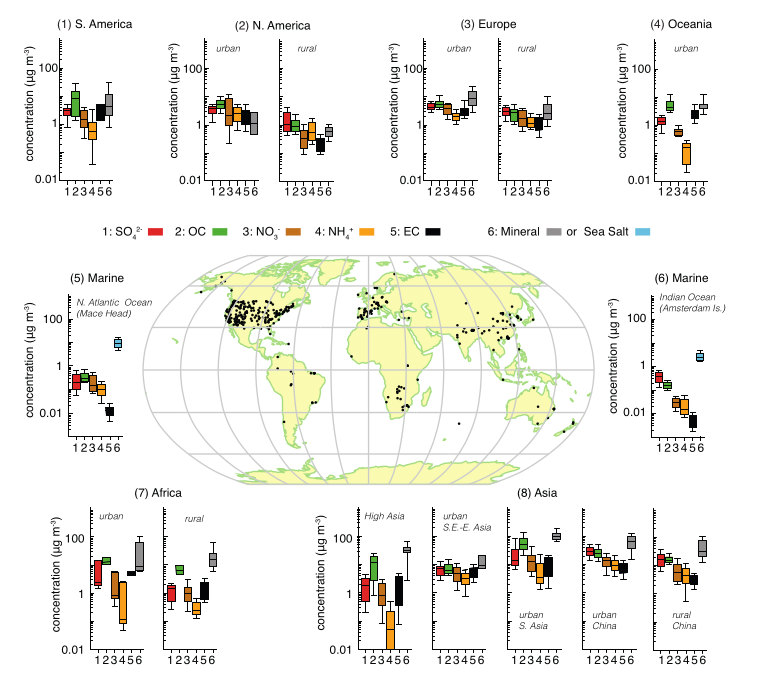
\includegraphics[width=1.0\linewidth]{chapter01/composition_chimique.png}
    \caption{Composition chimique majeure de la masse des \PMdix{} pour différentes
        typologies de sites de prélèvement. Crédit: \cite[figure 7.13]{boucherClouds2013},
        agrégeant 113 études sur au moins une année de prélèvement, entre 1993 et 2012.}%
    \label{fig:chapter01/composition_chimique}
\end{figure}

\subsection{Impacts des aérosols sur l'écosystème terrestre}%
\label{sub:impacts_des_aérosols_sur_l_écosystème_terrestre}

\subsubsection{Impacts climatiques}%
\label{ssub:impacts_climatiques}

Les aérosols sont des éléments essentiels de la machine climatique terrestre de par leur
interaction avec le rayonnement solaire et donc leur impact sur le bilan radiatif de la
Terre. Ils sont également essentiels de par leur interaction très forte avec la dynamique
des nuages, au point que les rapports du GIEC traitent dans le même chapitre les nuages et
les aérosols.

\paragraph{Impact radiatif}%
\label{par:impact_radiatif}

De par leur faible taille, les aérosols diffusent le rayonnement incident. Ils agissent
donc comme ``bouclier thermique'', ré-émettant une partie du flux solaire entrant dans
l'espace, conduisant ainsi à un refroidissement de l'atmosphère.  Cependant, les aérosols
absorbent aussi une partie du rayonnement incident, ce qui augmente l'agitation thermique
et donc conduit à un réchauffement du climat.  Ces deux effets antagonistes agissent de
concert à différentes altitudes de l'atmosphère et dépendent de la composition chimique
des aérosols.  Enfin, le dépôt des aérosols et notamment du \textit{black carbone} sur la
neige ou les glaces des banquises induit un effet bien connu de rétroaction positive. Le
carbone diminue l'albédo et absorbe le rayonnement normalement réémis par les surfaces
blanches, augmente donc localement la température et fait fondre la glace, découvrant
ainsi des surfaces plus sombres (roche ou océan) absorbant davantage de rayonnement,
conduisant à un réchauffement accru, et ainsi de suite.

\paragraph{Impacts sur la dynamique des nuages}%
\label{par:noyaux_de_condensation_des_nuages}

Les aérosols, grâce à leur taille et leurs ions, permettent en revanche de baisser
l'énergie d'activation nécessaire à l'agrégation de la vapeur d'eau sous forme liquide en
gouttelettes, puis goutte, facilitant l'apparition des nuages. Ainsi, les aérosols agissent
comme noyaux de condensation des nuages (CCN pour \textit{cloud condensation nuclei}).
Certes, les nuages empêchent les infrarouges terrestres de repartir vers l'espace, mais
présentent également un albédo élevé renvoyant une grande partie du rayonnement à courte
longueur d'onde du Soleil vers l'espace. L'effet observé est donc un refroidissement de
l'atmosphère.
Aussi, pour une même quantité d'eau, le nombre de CCN disponibles conditionne la taille des
gouttelettes des nuages donc la taille de ceux-ci, leur durée de vie et probabilité de se
transformer en nuage précipitant.

\paragraph{Impacts sur le dérèglement climatique en cours}%
\label{par:impacts_sur_le_dereglement_climatique_en_cours}

Du fait de ces différents aspects antagonistes, très brièvement exprimés ci-dessus,
l'impact total des aérosols sur le climat n'est connu qu'avec une incertitude élevée. 

La contribution des aérosols à la différence du forçage radiatif entre 1750 et 2011 s'estime entre
\SIrange[range-phrase=~et~]{-0.77}{0.23}{\W\per\m\squared} (pour un forcage total actuel
de \SI{2.29}{\W\m\squared}), avec un forçage négatif pour
les poussières minérales, le sulfate, nitrate et carbone organique, mais positif pour le
carbone suie.  Quant à leur rôle sur la dynamique des nuages, il s'estime entre
\SIrange[range-phrase=~et~]{-1.33}{-0.06}{\W\per\m\squared}, mais présente des
incertitudes plus élevées du fait de la complexité à prendre en compte ces phénomènes dans
les modèles de climat. C'est actuellement le forçage radiatif le moins bien connu de la
machine climatique Terrestre.

\subsubsection{Impacts environnementaux}%
\label{ssub:impacts_environnementaux}

La durée de vie des aérosols dans l'atmosphère entre leur émission et leur déposition est
de plusieurs jours pour la majorité d'entre eux. Dans ce délai, la circulation atmosphérique les déplace sur des
distances pouvant atteindre plusieurs milliers de kilomètres. Il n'est pas rare par exemple en
Europe d'avoir des épisodes de dépôts de sable provenant du désert saharien. Ce
déplacement longue distance d'aérosols est même un des mécanismes clef de certains
\textit{bloom}
de phytoplancton, en apportant d'importantes quantités de nutriments à la surface de l'océan 
(métaux et phosphate notamment).
Autre exemple marquant, le nitrate, élément limitant de la croissance des
plantes en prairie d'altitude, est apporté en partie par
déposition de nitrate d'ammonium particulaire provenant du transport longue
distance~\autocite{bourgeoisFoliar2019}.

Plus spectaculaire, les cendres volcaniques relarguées dans l'atmosphère suite à de
violentes éruptions, en plus de leur impact climatique potentiel, peuvent occasionner des
pluies acides du fait de la présence en quantité de sulfate dans ces cendres.

Ces phénomènes présentent à quel point les aérosols et leur composition chimique variée
impactent directement de nombreux écosystèmes terrestres, et ce, qu'ils proviennent de sources
anthropiques comme c'est le cas pour le nitrate, ou de sources naturelles.

\subsection{Impacts sanitaires}%
\label{sub:impacts_sanitaires}

L'impact sanitaire des aérosols sur la population humaine a commencé à être
un sujet de recherche suite à l'industrialisation et aux épisodes de ``smog'' causant la
mort de nombreuses personnes à Engis (Meuse, Belgique) en 1930, Donora (Pennsilvanie, USA)
en 1948 ou encore le plus connu ``Great smog of London'', en 1952. Durant ces épisodes de
pollutions, il est important de noter que la sur-mortalité due à l'exposition aigüe
durant l'épisode est très importante (jusqu'à 3 fois supérieure à la normale
pour le smog de Londres), mais que la surmortalité persiste dans les mois qui suivent
--pendant près d'un an pour le smog de Londres-- alors même que les niveaux de pollution
étaient revenus à leurs états antérieur à décembre 1952 \autocite{bellReassessment2001}.  Ces
épisodes de pollution intenses marquent le début de la prise de conscience par la
population de la problématique de la pollution de l'air et ont conduit à la première
législation anglaise en matière de qualité de l'air en 1956 avec le \textit{Clean Air
Act}. Aussi, des programmes de mesures de la qualité de l'air pour différents polluants
ont émergés et les actions misent en œuvre au niveau national et international ont permis
en depuis Europe une amélioration très sensible de la qualité de l'air
(Figure~\ref{fig:chapter01/tendance_polluants}).

\begin{figure}[ht]
    \centering
    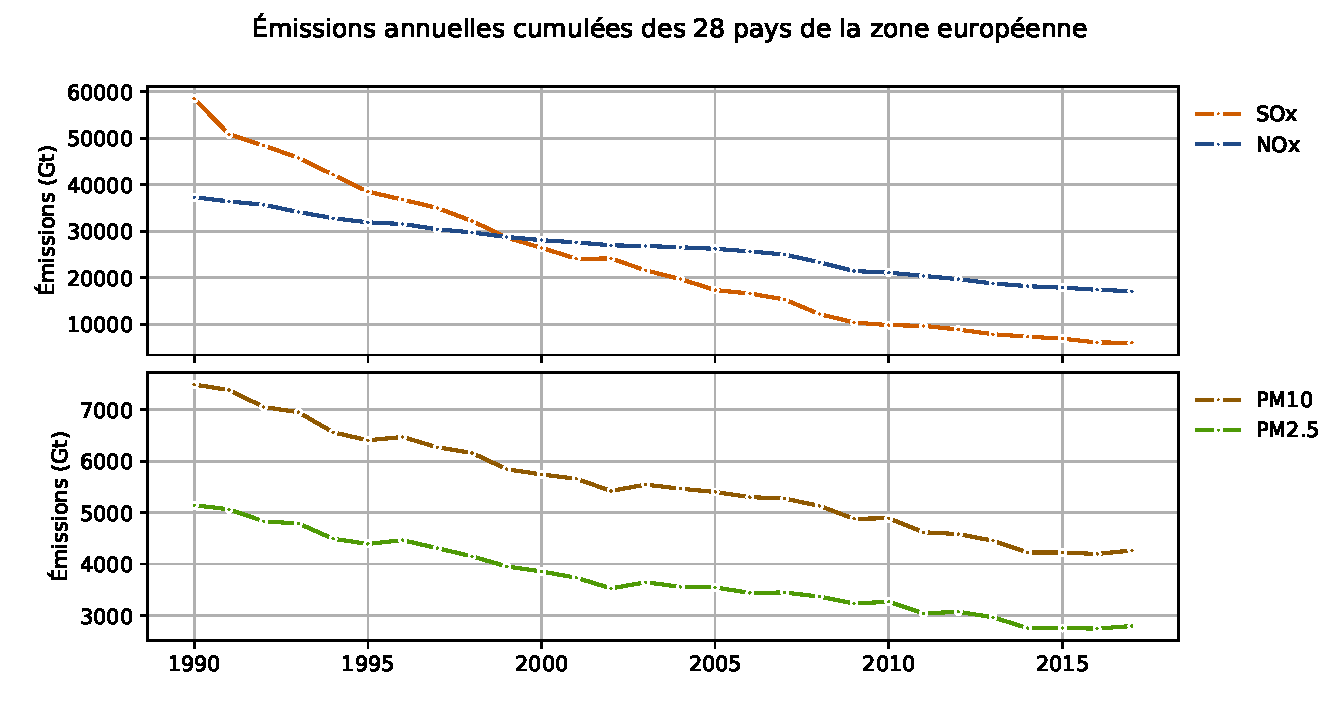
\includegraphics[width=0.9\linewidth]{chapter01/tendance_polluants.pdf}
    \caption{Évolution temporelle des émissions cumulées des 28 pays de la zone européenne
    depuis 1990, indiquant une prise de conscience et une diminution des émissions de
    différents polluants gazeux (\ce{SO_x} et \ce{NO_x}) et particulaires (\PMdix{} et \PMdc). Données
issues de \textit{National emissions reported to the Convention on Long-range
Transboundary Air Pollution (LRTAP Convention)}, ©European Environment Agency (EEA).}%
\label{fig:chapter01/tendance_polluants}
\end{figure}


Cependant, la qualité de l'air (incluant les aérosols, mais également les
composés gazeux comme les \ce{NO_x} ou l'ozone) demeure actuellement la 5\ieme{} cause de
mortalité dans le monde, représente un décés sur dix et est catégorisée ``cancérogène
certain'' par le CIRC depuis 2013. En Europe, pour l'année 2013, c'est
ainsi \num{800000} personnes qui sont décédées des suites de maladies cardiovasculaires,
cancer, pneumonie… directement attribuables à la qualité de l'air
\autocite{worldhealthorganizationAmbient2016}. Récemment, \cite{lelieveldLoss2020}
estiment qu'en moyenne et à travers le monde, c'est \num{2.9} ans de vie perdue par personne
qui sont imputables à la pollution de l'air, dont \num{1.7} ans ``évitables'' car provenant
directement de sources anthropiques.

En termes de bilan financier, la banque mondiale en collaboration avec l'Institute for
Health Metrics and Evaluation (IHME) de l'université de Washington estimait que le coût
associé aux décés prématurés de la seule année 2013 s'évaluait à plus de \$5.11 trillions
de dollar dans le monde~\autocite{worldbankCost2016}.

Afin de limiter cet impact sanitaire, de nombreux pays ont définis des seuils de
concentrations de différents composés (voir Tableau~\ref{tab:seuil_PM} pour les PM).
Seulement ces seuils sont différents d'une institution à une autre. Par exemple, entre
2015 et 2017, le seuil de concentration journalière recommandé pour les \PMdix{} par
l'union européenne (\SI{50}{\ugm} en moyenne journalière) était dépassé pour 13 à
19~\% de la population européenne, mais cette proportion augmente entre 42 et 62~\% si
l'on prend en compte le seuil recommandé de l'OMS de \SI{20}{\ugm} en moyenne
annuelle~\autocite{europeanenvironmentagencyAir2019}.  De plus, il est à noter qu'il
n'existe pas de seuil à partir duquel l'exposition aux PM est inoffensive.

\begin{table}[ht]
    \begin{ThreePartTable}
        \centering
        \caption{Seuils de concentration de PM recommandés par différents organismes.}
        \label{tab:seuil_PM}
        \begin{tabular}{ccSc}
            \toprule
            Organisme       & Polluant & {Concentration (\si{\ugm})} & Période \\
            \midrule
            OMS\tnote{a}    & \PMdc  & 10 & moyenne annuelle       \\
            OMS\tnote{a}    & \PMdc  & 25 & moyenne sur \SI{24}{h} \\
            OMS\tnote{a}    & \PMdix & 20 & moyenne annuelle       \\
            OMS\tnote{a}    & \PMdix & 50 & moyenne sur \SI{24}{h} \\
            Europe\tnote{b} & \PMdc  & 25 & moyenne annuelle       \\
            Europe\tnote{b} & \PMdc  & 20 & moyenne sur 3 ans      \\
            Europe\tnote{b} & \PMdix & 40 & moyenne annuelle       \\
            Europe\tnote{b} & \PMdix & 50 & moyenne sur \SI{24}{h} \\
            France\tnote{c} & \PMdc  & 25 & moyenne annuelle       \\
            France\tnote{c} & \PMdix & 50 & moyenne sur \SI{24}{h} (\SI{<35}{jour\per an}) \\
            France\tnote{c} & \PMdix & 40 & moyenne annuelle \\
            \bottomrule
        \end{tabular}
        \begin{tablenotes}
        \item[a] OMS air quality guideline \cite{worldhealthorganizationWHO2006}
        \item[b] Directive 2008/50/EC \cite{officialjournaloftheeuropeanunionDirective2008}
        \end{tablenotes}
    \end{ThreePartTable}
\end{table}

\section{Détermination des sources d'émission des PM}%
\label{sec:source_apportionment_of_pm}

Comme nous l'avons vu, les sources d'aérosols sont très diverses.
Afin de pouvoir avoir un impact sur les concentrations de polluants via des
réglementations, il est primordial de
retracer leur provenance. Plusieurs techniques d'analyses existent, qu'elles soient purement
physiques ou géochimiques.

\subsection{Modèle d'attribution des sources}%
\label{sec:source_apportionment_model}

Afin d'estimer la contribution de chaque source de PM en un point donné, il est possible
d'utiliser 2 grandes familles de modèles d'attribution des sources (\textit{source
apportionment} (SA)). La première est fondée sur notre connaissance des
émissions et de la météorologie et calcule les réactions physico-chimiques depuis les
sources jusqu'au lieu d'étude (modèle dit de chimie-transport (\textit{chemical transport
model} (CTM)) alors que la deuxième s'évertue à mesurer en un point donné
la chimie des PM et par traitement statistique, attribue à différentes sources ou
``facteurs'' leurs contributions aux concentrations observées (modèle dit récepteur
(\textit{receptor model} RM)).

\subsubsection{Modèle déterministe de chimie-transport}%
\label{ssub:modele_deterministe_de_chimietransport}

\paragraph{Présentation}%
\label{par:presentation}

Les modèles déterministes s'appuient sur l'inventaire des sources d'émissions sur la
région étudiée. Ces cadastres d'émissions sont regroupés en catégories \textit{Selected
Nomenclature for reporting of Air Pollutants} (SNAP) représentant chacune un secteur
d'activité : Énergie, Procédés industriels, Agriculture, Déchets, Autres et enfin
Naturelle.
Chacune de ces catégories possédant évidemment des sous-catégories raffinant la
classification (par exemple, les émissions de l'aviation civile des avions de plus de \SI{100}{m} de
long se retrouvent dans le SNAP 080503 (ou \textit{Nomenclature For Reporting} (NFR)
1.3.A.c) autrement dit Énergie - Combustion - Aviation - Aviation civile de plus de
\SI{100}{m})~\autocite{europeanenvironmentagencyEMEP2019}.
À chacune de ces SNAP est associé un profil d'émission (\ce{O3}, \ce{SO2}, \ce{NO_x}, \ce{NH3}, \PMdix, \PMdc,
VOC principalement), obtenu soit par mesure directe, soit par calcul.

Vient ensuite un inventaire de ces sources d'émissions sous forme de cadastre géographique
et temporel. Notamment la \textit{Convention on Long-Range Transboundary Air
Pollution} (LRTAP) implémenté par l'\textit{European Monitoring and Evaluation Program}
(EMEP) sous l'égide de \textit{United Nations Economic Commission for Europe} (UNECE)
prévoit que les différentes parties prenantes à cette convention (i.e. les pays membres)
présentent un rapport de leurs émissions régulièrement à l'EMEP.

Il est alors possible de construire des modèles déterministes de dispersion et de
réaction des polluants, en couplant un modèle de diffusion résolvant les équations de la
physique de l'atmosphère (Navier-Stoke, turbulence, rayonnement, etc) avec un modèle
physico-chimique faisant évoluer les composés gazeux et particulaires, incluant leurs
émissions, dépôts, interaction physico-chimique, etc. Pour n'en citer que quelques-uns : 
Community Multi-scale Air Quality (CMAQ)\footnote{CMAQ: \url{https://www.epa.gov/cmaq}},
Comprehensive Air Quality Model with Extensions (CAMx)\footnote{CMAx : \url{http://www.camx.com/}},
WRF-Chem\footnote{WRF-chem : \url{https://www2.acom.ucar.edu/wrf-chem}},
Chimère,
LOTOS-EUROS...

La raison de la pluralité de ces modèles provient des différentes paramétrisations
possibles des équations physiques, mais également des choix conceptuels de recherche.

\paragraph{Limitations}%
\label{par:limitations}

Comparaison Chimire-DECOMBIO : \cite{bessagnetHigh2020}
\todo{à faire}

\paragraph{Source apportionment}%
\label{par:source_apportionment}

Concernant l'attribution des sources, il est possible d'utiliser deux techniques au sein
des CTM:

\begin{enumerate}
    \item Faire une première simulation incluant toutes les sources d'émissions (référence
        ou témoin), puis une deuxième simulation avec une source d'émission en moins. La
        différence reflétant l'impacte de la source supprimée sur les concentrations
        ambiantes (technique dite de force-brute);
    \item Garder en mémoire la provenance de chacune des espèces chimiques lors des
        schémas réactionnels (technique dite de \textit{source labelling} ou \textit{tagged species}).
\end{enumerate}

Seulement, du fait des nombreux processus non linéaires, la suppression d'une source
d'émission aura des répercussions beaucoup plus complexes que la simple diminution des
concentrations propres à cette source (par exemple, des NOx pourraient ne pas passer en
phase particulaire du fait d'un manque d'ammoniac, ou inversement). 
% TODO: élaborer ou supprimer cette partie
%La première technique correspond donc à se demander 
%\begin{quote}
%    Si les émissions de cette source sont diminuées ou supprimées, quels impacts cela va-t-il
%    avoir sur les concentrations finales ?
%\end{quote}
%alors que la deuxième répond à
%\begin{quote}
%    Dans la concentration ambiante de PM, à combien s'estime la contribution de cette source
%    d'émission ?
%\end{quote}
%Ce sont bien deux questions différentes avec leurs légitimités propres.
La seconde technique a commencé été implémentée plus récemment dans certains
CTM~\autocite{wangDevelopment2009,wagstromDevelopment2008,kranenburgSource2013,brandtContribution2013}
et elle est détaillée dans le rapport de~\cite{mirceaEuropean2020}. Elle présente également
l'avantage de pouvoir tagguer non seulement les sources des espèces chimiques, mais
également leur provenance géographique, c'est-à-dire leur lieu d'émission.

Cependant, l'utilisation des CTM présente certaines limites du fait de leur complexité.
Notamment, il semble illusoire de pouvoir un jour inclure toutes les réactions chimiques
possibles dans les modèles déterministes. Par exemple, les interactions aérosols/neiges ou
même plus simplement les interactions aérosol nuages et la chimie aqueuse qui s'y produit
ne sont pas encore complètement comprises ni bien représentées dans ces modèles.

Quand bien même ce serait le cas --car les modèles réactionnels sont de plus en plus
poussés--, il faudrait alors avoir des inventaires d'émissions beaucoup plus complets et
précis temporellement, avec aucune certitude d'un oubli potentiel d'une source non prise
en compte. Ce sont par exemple, une industrie locale non-encore répertorié, la sous-estimation de
la contribution d'un écosystème, une consommation de bois de chauffage individuel non
inventoriée, etc.

Aussi, la limitation physique des modèles météorologiques se retrouvent dans les CTM. Il
est donc compliqué d'envisager, du fait du coût de calcul et de stockage, une simulation à
\SI{10}{\m} de résolution spatiale (ou moins), ce qui serait cependant nécessaire pour
appréhender correctement des phénomènes précis, comme les inversions thermiques des
vallées alpines.

\subsubsection{Modèles récepteurs}%
\label{ssub:model_recepteur}

À l'inverse des CTM, il est possible d'estimer les sources contribuant aux concentrations
ambiantes en un lieu donné sans la moindre information météorologique ou simulation
déterministe. Pour cela, il convient de faire des prélèvements sur le lieu d'étude,
d'analyser la chimie que l'on y trouve et retrouver à l'aide d'un modèle statistique
les différents profils de source et leurs contributions, ce qui peut se traduire en
particulier par l'équation d'équilibre des masses
\begin{align}
    \label{eq:mass_balance}
    X &= G \cdot F
\end{align}
où $X$ est la matrice de dimension $n\times m$ des observations, $G$ est la matrice des
contributions de taille $n\times p$ et $F$ la matrice des profils de taille $p \times n$,
avec $n$ le nombre d'échantillons, $m$ le nombre de variables chimiques mesurées et $p$ le
nombre de facteurs.
Un \textit{facteur} peut être une source d'émission (combustion de biomasse par exemple),
mais également regrouper des espèces chimiques provenant d'un même processus secondaire
(nitrate d'ammonium par exemple).
Il est courant d'exprimer $X$ en \si{\ugm}, $G$ en \si{\ugm} ou concentration
normalisée~\si{[-]} et $F$ en \si{\micro\g\per\micro\g} ou \si{\ugm}.

Si l'on mesure $X$, ce qui nous intéresse ici est de connaître $G$ ou $F$.
Si l'on admet que l'on connait a priori les profils d'émissions possibles, alors $F$ est
connue et l'on cherche à estimer $G$. Le modèle de déconvolution adapté est alors le
\textit{Chemical Mass Balance} (CMB). À l'opposé, on peut n'avoir aucune information a
priori à la fois sur les contributions et les profils d'émissions. On utilisera alors le
modèle de déconvolution \textit{Positive Matrix Factorization} (PMF).

Ces 2 types de modèles statistiques sont aux deux extrêmes d'un spectre de modèles de
déconvolution, depuis une information ``absolue'' des profils de sources à une absence
totale d'information sur ces mêmes profils.  Il existe cependant un continuum entre ces
deux pôles (voir Figure~\ref{fig:chapter01/source_apportionment_methods}), et de nombreux
modèles ont été développés et améliorés depuis la première étude de SA de
\cite{colucciAutomotive1965} utilisant la ``simple'' corrélation entre le \ce{CO} et
le plomb et benzo(a)pyrène.  Une revue détaillée et historique du fonctionnement de ces
différents modèles peut-être retrouvées dans les articles de
\cite{henryHistory1997,vianaSource2008,belisCritical2013,hopkeReview2016}.

\begin{figure}[ht]
    \centering
    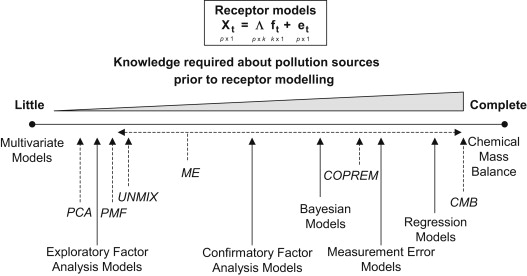
\includegraphics[width=0.7\linewidth]{chapter01/source_apportionment_methods.png}
    \caption{
        Connaissances a priori nécessaires pour les différents modèles de SA existant,
        depuis la simple analyse de facteur par ACP au modèle CMB. Crédit :
        \cite{vianaSource2008} adaptée de \cite{schauerCharacterization2006}
    }%
    \label{fig:chapter01/source_apportionment_methods}
\end{figure}

\subsubsection{Chemical mass balance CMB}%
\label{ssub:chemical_mass_balance_cmb}

Le principe du CMB est de déterminer la contribution $G$ d'un nombre de sources
aux profils chimiques $F$ prédéfinis aux concentrations ambiantes $X$. Il est donc
nécessaire de connaître les signatures chimiques des sources utilisées.

Afin d'utiliser le modèle CMB --mais également pour d'autres buts-- l'US EPA construit
depuis 1988 la base de donnée SPECIATE~\autocite{simonDevelopment2010}, répertoriant
différents profils d'émission, dont la 5\ieme{}
version a été publiée en 2019~\autocite{u.s.environmentalprotectionagencySPECIATE2019}.
Seulement, ces profils sont représentatifs des sources présentes aux États-Unis et sont
très certainement non transposables à d'autres régions du monde.
En Europe, il existe depuis 2016 une base de données similaire,
SPECIEUROPE~\autocite{pernigottiSPECIEUROPE2016}, compilant des mesures à l'émission et
les résultats d'autres types d'étude permettant d'estimer la signature chimique des
profils d'émission.

Cependant, des erreurs ou variabilités locales spécifiques au site récepteur sur ces
profils peuvent conduire à une estimation erronée des contributions finales des
différentes sources en utilisant le modèle CMB.
Aussi, il est nécessaire de choisir ou d'agréger certains des >3000 profils de sources
différents répertoriés afin de restreindre à une valeur réaliste le nombre de sources
potentielles en un lieu donné.
Enfin, les processus secondaires sont mal pris en compte dans ce type modèle. L'exemple typique
concerne l'aérosol inorganique secondaire sulfaté, représenté comme un mélange de sulfate
et d'ammonium. Or ce facteur secondaire est souvent associé en réalité à de la matière
organique ou d'autres espèces sulfatées.

\subsubsection{Positive Matrix Factor PMF}%
\label{ssub:pmf}

Un modèle beaucoup plus agnostique que le CMB pour résoudre l'équation de conservation de
la masse a été développé par~\cite{paateroPositive1994}. Dans cette formulation,
seule la matrice d'observation $X$ est connue, et les matrices de contribution $G$ et des
profils chimiques $F$ sont inconnues.

\paragraph{Formulation mathématique}%
\label{par:formulation_mathématique}

Le principe de la PMF provient initialement de la recherche sur le \textit{machine
learning}, et plus particulièrement de l'analyse factorielle appliquée au problème
bilinéaire $X=G\times F$. L'intérêt initial est de permettre une réduction
dimensionnelle sans perte d'information. Par exemple, en informatique, une image de $n$
par $m$ pixels forme une matrice $n\times m$ éléments. S'il est possible de retrouver
cette matrice par multiplication de 2 matrices $G$ ($n\times p$) et $F$ ($p \times m$),
alors la quantité d'information stockée dans $G$ et $F$ est $n
\times p + p \times m = p \times (n + m)$. Ainsi, tant que $p < \frac{n\times m}{n+m}$,
alors le nombre d'éléments de $G\times F$ est toujours inférieur au nombre d'éléments de
$X$, permettant un gain de mémoire de plus en plus important au fur et à mesure que $n$ et
$m$ augmentent.
Tout le problème réside en le fait de trouver la décomposition de $X$ en minimisant
l'erreur engendrée par cette simplification.

Aussi, on observe que la formulation $X = G\cdot F$ est similaire à celle de
la conservation de la masse (Eq.~\ref{eq:mass_balance}). Ce problème peut-être résolu par
analyse en composante principale (ACP), seulement, le résultat obtenu présente des
combinaisons linéaires (additive et soustractive) des différents composants. Cette possible
négativité des composants n'a pas de sens dans beaucoup de domaines physiques, y compris en
géochimie. \cite{paateroPositive1994} présentent donc une nouvelle méthode de
déconvolution, implémentant une contrainte de non-négativité, nommée \textit{Positive Matrix
Factorization} (PMF). 

La formulation est la suivante : étant donné une matrice d'observation $X$ de taille
$n\times m$, une matrice associée des incertitudes $U$ de taille $n \times m$ et un rang
$p$, alors 
\begin{align}
    \label{eq:pmf_formulation}
    X &= G \cdot F + E \\
    \forall i,k,j &, G_{ik}\geq 0 \text{ et } F_{kj}\geq 0\\
    Q &= \sum_{i=1}^n\sum_{j=1}^m E_{ij}^2/U_{ij}^2\label{eq:Qfunction}\\
    {Q, F} &= \argmin_{G,F} Q.
\end{align}

Différents algorithmes de résolution du système Eq.~\ref{eq:pmf_formulation} ont été développés.
L'implémentation initiale de~\cite{paateroLeast1997} a été améliorée pour pouvoir
ajouter des contraintes sur les matrices $G$ et $F$, notamment grâce au solveur
\textit{multi-linear engine} (ME-2) \autocite{paateroMultilinear1999}. En effet, il
n'existe pas de solution unique au problème Eq.~\ref{eq:pmf_formulation}, notamment, car le
système est invariant par rotation:
\begin{align}
    \label{eq:rotationalambiguity}
    X   &= G \cdot F + E \\
        &= (G \cdot T) \cdot (T^{-1} \cdot F) + E\\
        &= G' \cdot F' + E
\end{align}
et ainsi une infinité de solutions coexistent. 

\paragraph{Interprétabilité du modèle PMF}%
\label{par:interpretabilite_du_model_PMF}

L'avantage de la PMF réside en le fait que l'algorithme n'est pas fondé sur la
corrélation entre variables, comme c'est le cas de l'ACP, mais bien en la formation d'un
modèle additif linéaire de ce qui est observé.
\begin{quote}
    We shall not be satisfied in finding some correlations, we wish to form a quantitative
    model of what was observed! \autocite{paateroPositive1994}
\end{quote}

Il a été montré que la PMF est capable d'extraire des informations partielles cohérentes des
données là où l'ACP n'est qu'une représentation holistique~\autocite{leeLearning1999}. Par
exemple, appliquée à la reconnaissance d'image faciale, la PMF déconvolue les visages en
sous partie (bouche, sourcils, front, etc) alors que d'autres méthodes ``se contentent''
d'une approche globale de l'information et où seules les premières dimensions portent
l'information nécessaire à la reconstruction du signal (voir
figure~\ref{fig:chapter01/NMFvsPCA}).

\begin{figure}[ht]
    \centering
    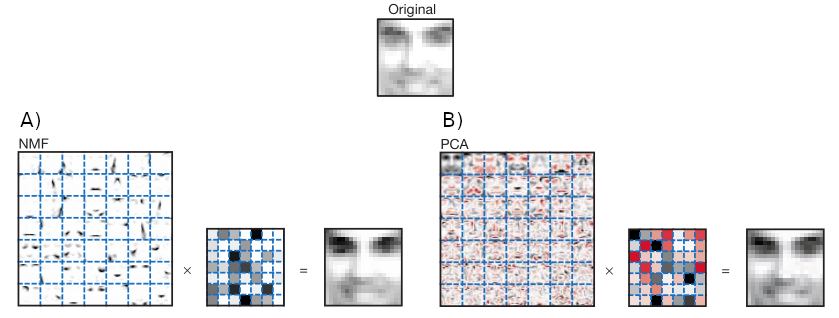
\includegraphics[width=1.0\linewidth]{chapter01/NMFvsPCA.png}
    \caption{Analyse factorielle par PMF (ou NMF pour \textit{non-negative matrix
    factorization}) et ACP d'une banque d'image de 2429 images en niveau de gris de 19
    pixels par 19 pixels. Les deux techniques essaient de reproduire l'image originale en
    fonction de leur apprentissage.
    \textbf{A)} Le rang de la PMF est $p=49$, correspondant aux 49
    représentations des $19\times19$ images à gauche, chacune étant un facteur de la
    matrice $F$, et leurs ``contributions'' respectivement identifiées par le carré de 7 par
    7 en niveau de gris, à droite.
    \textbf{B)} Analyse en composante principale, le carré de gauche représentant les 49
    vecteurs propres et celui de droite les 49 valeurs propres.
    Les échelles de couleurs sont : rouges pour les coefficients négatifs, noirs pour les
    coefficients positifs.
    Figure adaptée de \cite{leeLearning1999}}%
    \label{fig:chapter01/NMFvsPCA}
\end{figure}

\paragraph{Applicabilité en science de l'atmosphère}%
\label{par:applicabilité_en_science_de_l_atmosphère}

Dans le cas qui nous intéresse ici, cela signifie que chacun des vecteurs de la matrice
$F$ correspond à un profil chimique, en \si{\ugm}, indépendant des autres profils, et
que la matrice $G$ représente la contribution de chacun de ces profils au jour
considéré, de manière cohérente avec l'équation de conservation de la masse.

Puisque la PMF ne nous donne qu'un profil chimique, certains de ces profils représentent
directement une source d'émission, et d'autres correspondent à un ensemble de processus
conduisant à un profil chimique stable. On ne peut donc pas appeler ``source'' tous les ensembles
identifiés par la PMF puisque certains ne sont pas à proprement parler émient tels quels et
proviennent de processus physico-chimiques ayant eu lieu après les émissions de ces
composés.
Le terme de \textbf{facteur} est donc utilisé pour désigner un profil chimique et sa
contribution.

Le modèle PMF est maintenant très largement utilisé, et son application a été grandement
favorisée
par son implémentation dans le logiciel de l'EPA: EPA PMF5.0~\autocite{norrisEPA2014}.
Si l'EPAPMF5 est massivement utilisée pour les données provenant d'analyses de
filtres, l'utilisation pour des spectres de masse provenant de mesures d'AMS est facilitée par
l'utilisation du logiciel SoFi~\autocite{canonacoSoFi2013}. Ces deux logiciels utilisent
le solveur ME-2 pour résoudre le système d'équation de la PMF.

\paragraph{Estimation des incertitudes}%
\label{par:incertitudes}

Il existe différent type d'incertitudes pour ce modèle : 1) la sensibilité aux données
d'entrée (sur ou sous représentation de certains événements : impact d'un point
``extrême'' par exemple) et 2) l'incertitude rotationelle~\autocite{brownMethods2015}.

La première incertitude est évaluée à travers une méthode de \textit{bootstrap} consistant
à ré-échantilloner par blocs la matrice des observations $X$, à reconduire une simulation
PMF et à faire correspondre chacun des nouveaux facteurs obtenus à ceux qui lui sont le
plus proche dans la simulation initiale.
On obtient ainsi une incertitude sur les profils chimiques mais également sur les
contributions temporelles.
Cela permet aussi d'évaluer si la solution initiale était statistiquement peu fréquente
dans l'espace des possibles ou si au contraire elle correspond à minimum de la fonction
coût $Q$ relativement commun.

L'incertitude rotationnelle s'estime par méthode dite de \textit{displacment}. La gamme des
valeurs possibles de chacune des espèces chimiques de chacun des profils correspondant à
une variation de la fonction coût $Q$ inférieur à une quantité donnée (par exemple $dQ =
0.5\%$) est évaluée. Toutes ces valeurs sont alors possibles, et correspondent donc à
l'incertitude rotationnelle de la solution.

\paragraph{Limitation de l'ambiguïté et contrainte géochimique}%
\label{par:limitation_de_l_ambiguité_et_contrainte_géochimique}

Cependant, il est possible de limiter l'ambiguïté rotationnelle et donc de limiter
l'incertitude de la solution par l'ajout de contraintes géochimiques au modèle statistique.
Cela est rendu possible par le solutionneur ME-2 qui permet notamment l'ajout de contraintes
sur les matrices $G$ et $F$, limitant de fait le nombre de rotations possibles de ces
matrices. Ce faisant, l'utilisateur rajoute de la connaissance a priori au modèle qui
était jusqu'alors purement statistique. C'est pourquoi dans la
figure~\ref{fig:chapter01/source_apportionment_methods} le ME-2 n'est pas à l'extrémité de
l'axe : l'utilisateur rajoute de la connaissance sur les profils ou contributions
temporelles des différents facteurs.

L'ajout de ces contraintes limites de fait les rotations possibles des matrices $F$ et
$G$, conduisant non-seulement à des solutions géochimiquement plus compréhensibles mais
aussi à une incertitude plus faible des profils des différents facteurs.

\paragraph{Subjectivité de l'expérimentateur}%
\label{par:subjectivité_de_l_expérimentateur}

L'utilisateur a donc 3 paramètres à choisir manuellement : les observations $X$, leurs
incertitudes $U$ (utilisée pour le calcul de la fonction objective $Q$
Eq.~\ref{eq:Qfunction}) et le nombre de facteurs (ou rang) $p$. Chacun de ces paramètres
influencera la solution finale obtenue et provient de la subjectivité de l'expérimentateur:
quelles espèces chimiques utiliser ? garder ou non ce jour d'observation ``extrême'' ?
quelles incertitudes pour quelles espèces ? combien de facteurs accepter dans la solution
retenue ?

Une inter-comparaison européenne de modèle récepteur utilisant une base de donnée
constituée sur le site de Lens a été conduite par
\cite{belisEvaluation2020}. Les 38 études des participants bénéficiaient de
la même base de données. Cependant, non seulement le nombre de facteurs retrouvés varie de 5 à 12 mais 
les contributions temporelles, bien que globalement concordante, varient entre les
différentes études, comme le montre les z-scores de la figure~\ref{fig:chapter01/belisEvaluation2020_fig2a}
\footnote{Le z-score représente ici une distance entre les contributions temporelles de
    chacune des sources des différentes études à la moyenne de celles-ci, définie par 
    \begin{align}
        \label{eq:z-score}
        z = \frac{x-X}{\sigma}
    \end{align}
    où $x$ est une série temporelle d'un facteur, $X$ la moyenne des séries temporelles de
    ce facteur issue des différentes études et $\sigma$ définie comme $0.5\times X$
    \parencite{pernigottiDeltaSA2018}.
}.

Cette diversité s'explique par le \textbf{choix des variables utilisées par la PMF},
reposant finalement sur la ``connaissance d'expert'' de l'expérimentateur. En effet, toutes les données
d'entrée ne portent pas la même quantité information et l'ajout d'espèces traceuses de
sources particulières conduira à l'obtention d'un facteur relié à ces sources. Au
contraire, l'ajout trop important d'espèces n'apportant pas suffisamment d'information peut
déstabiliser statistiquement le modèle et résulter en une solution statistiquement faible
(peu de répétabilité, variance importante, etc) et de fait géo-chimiquement douteuse.
Aussi, le \textbf{choix des contraintes} à appliquer impliquera des solutions
nécessairement différentes. Là encore, ces contraintes sont issues de la connaissance a
priori de l'expérimentateur et sont donc en partie subjectives.

Enfin, l'identification des facteurs est laissé à l'appréciation de l'expérimentateur. Il
faut donc savoir identifier quel profil d'émission peut être responsable du facteur
observé. Cette nomenclature des facteurs est elle aussi subjective et non standardisée :
véhiculaire, émission routière, trafic routier, combustion diesel, etc. peuvent être
différents noms donnés au même profil, par différents utilisateurs.
% Des travaux récents, portés par le groupe FAIRMODE du JRC, portent notamment sur une
% harmonisation de cette nomenclature, à travers la construction d'une donnée européenne de
% profil de source standardisée et hierarchisé : SPECIEUROPE~\autocite{pernigottiSPECIEUROPE2016}.

Pour toutes ces raisons, la comparabilité des profils issus de différentes études PMF
est donc un sujet de recherche en cours, et sera abordée plus en détail dans le
chapitre~\ref{cha:approfondissement_des_connaissances_des_sources_des_pm}.

\begin{figure}[ht]
    \centering
    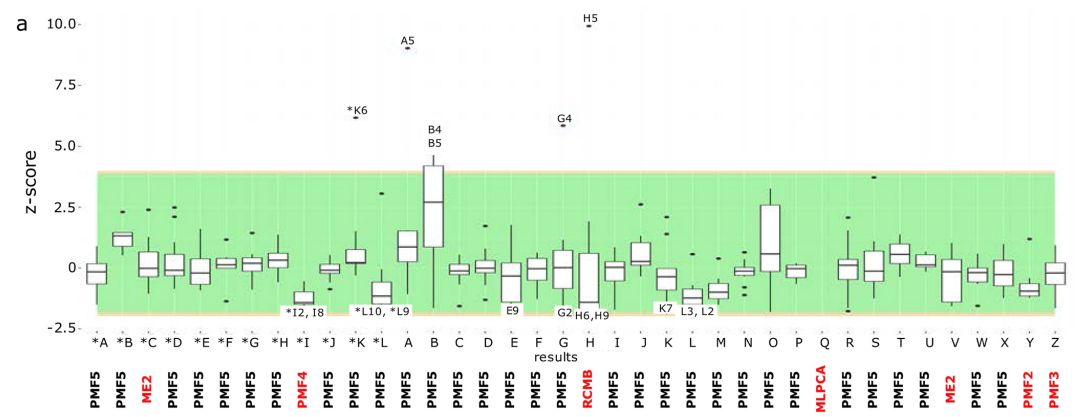
\includegraphics[width=1.0\linewidth]{chapter01/belisEvaluation2020_fig2a.png}
    \caption{Comparabilité des séries temporelles obtenues par les 38 différentes solutions
    sur l'étude de comparaison des modèles sources-récepteurs sur le site de Lens par
    rapport à la moyenne de l'ensemble des différentes études. L'axe X représente chacune des
    solutions des participants, et l'axe Y le z-score, mesure de la similitude des
contributions temporelles. La solution commune IGE-INERIS-EMD est la solution W.\\
Source: \cite{belisEvaluation2020}}%
    \label{fig:chapter01/belisEvaluation2020_fig2a}
\end{figure}

\subsection{Atouts et limitations des différents modèles récepteurs}%
\label{ssub:atouts_et_limitations_des_différents_modèles_récepteurs}

Les 3 types de modèles listés précédemment (CTM, CMB et PMF) ne sont pas les seuls
utilisés, mais représentent néanmoins la très grande majorité des études d'attribution
des sources. Leurs atouts et limitations sont repris dans le
tableau~\ref{tab:comparison_SA} et nous expliquerons dans cette partie plus en avant le
choix pour cette thèse du modèle PMF avec analyse chimique sur filtre.

\begin{table}[!ht]
    \begin{ThreePartTable}
        \centering
        \caption{Forces et limitations des différents modèles d'attribution des sources}
        \label{tab:comparison_SA}
        \footnotesize
        \begin{tabular}{cp{0.43\textwidth}p{0.43\textwidth}}
        \toprule
        Type & Atouts & Limitations \\
        \midrule
        CTM &
        \begin{itemize}[topsep=0pt, left=0pt, label={\unicodesymbols ✔}]
          \item Grande couverture spatiale et temporelle
          \item Comparaison facilité : sources identiques partout\tnote{a}
          \item Prévision à court et long terme
          \item[{\unicodesymbols ~}] Peu de subjectivité\tnote{b}
        \end{itemize}
            &
        \begin{itemize}[topsep=0pt, left=0pt, label={\unicodesymbols ✘}]
          \item Nécessite des cadastres d'émissions
          \item Nécessite un modèle météo
          \item Ne voit que ce qui est donnée des cadastres
          \item Variabilité temporelle des émissions peu robuste
          \item Nombre d'espèces chimiques limités
        \end{itemize}
        \\ \midrule
        CMB & 
        \begin{itemize}[topsep=0pt, left=0pt, label={\unicodesymbols ✔}]
          \item Spécificité du site potentiellement prise en compte
          \item Grand nombre d'espèces pouvant être utilisé
        \end{itemize}
            & 
        \begin{itemize}[topsep=0pt, left=0pt, label={\unicodesymbols ✘}]
          \item Faible représentativité spatiale et temporelle
          \item Prélèvement et analyses couteux (humain et financier)
          \item Profils des sources fixes et connu à l'avance
          \item Nécessite une base de connaissance de profils chimique
          \item Subjectivité de l'expérimentateur
        \end{itemize}
        \\ \midrule
        PMF &
        \begin{itemize}[topsep=0pt, left=0pt, label={\unicodesymbols ✔}]
          \item Pas besoin de connaissance a priori des sources
          \item Spécificités du site prise en compte
        \end{itemize}
            & 
        \begin{itemize}[topsep=0pt, left=0pt, label={\unicodesymbols ✘}]
          \item Faible représentativité spatiale et temporelle
          \item Prélèvement et analyses couteux (humain et financier)
          \item Nécessite des espèces traceuses
          \item Grand nombre d'échantillons requis
          \item Subjectivité de l'expérimentateur
        \end{itemize}
        \\
        PMF-AMS &
        \begin{itemize}[topsep=0pt, left=0pt, label={\unicodesymbols ✔}]
          \item Grande caractérisation de la matière organique
          \item Possibilité de résolution temporelle très fine (mesure on-line)
        \end{itemize}
            & 
        \begin{itemize}[topsep=0pt, left=0pt, label={\unicodesymbols ✘}]
          \item Difficultés d'interprétation
          \item Cible uniquement la matière non réfractaire
          \item Peu utile pour la réglementation
        \end{itemize}
        \\
        PMF-filtre &
        \begin{itemize}[topsep=0pt, left=0pt, label={\unicodesymbols ✔}]
          \item Large gamme de famille d'espèce chimique
          \item Directement applicable pour la régulation
          \item D'autres analyse possible sur le même filtre (potentiel oxydant par
              exemple)
        \end{itemize}
            & 
        % \begin{itemize}[topsep=0pt, left=0pt, label={\unicodesymbols ✘}]
        % \end{itemize}
        \\
        \bottomrule
        \end{tabular}
    \end{ThreePartTable}
\end{table}


\subsubsection{La PMF : modèle théoriquement le moins biaisé par l'information a priori}%
\label{ssub:choix_du_modèle_pmf}

Lorsque l'on s'intéresse à un site particulier, le contexte géographique peut nous donner
des indications sur les sources majoritaires. Seulement, prédéfinir à l'avance les sources
possibles résulte en un biais évident : on ne voit que ce que l'on s'attend à voir.
L'utilisation des CTM ou du CMB ne nous permet donc pas de découvrir de nouvelles sources
locales. Au mieux, le modèle échouera à reproduire les observations, ce qui indiquerait
une source ou un processus manquant.

Au contraire, la PMF étant totalement agnostique aux sources ou processus réels, les
facteurs déterminés reflètent les observations locales sans biais. Ainsi, l'ajout d'une
espèce peut conduire à découvrir et quantifier une nouvelle source d'émission ou processus
atmosphérique, jusqu'alors non prise en compte ou sous-estimée, comme nous le verrons dans
le chapitre~\ref{cha:approfondissement_des_connaissances_des_sources_des_pm}. À noter
également que la réciproque est vraie : la non-prise en compte d'une espèce chimique peut
conduire à ne pas identifier un facteur important, ayant un impact direct sur la
contribution des autres facteurs aux PM.
Toute la difficulté réside dans le choix des ``bonnes espèces'' et en l'interprétation de
ce modèle, fondé sur nos connaissances géochimiques.

\subsubsection{Analyses chimiques ou spectrométrie de masse}%
\label{ssub:analyses_chimiques_ou_spectrometrie_de_masse}

Comme expliqué précédemment, les PM sont composées en grande majorité de matière organique
--tout du moins dans les écosystèmes européens.  Devant la myriade d'espèces chimiques la
constituant, la caractérisation exhaustive de cette matière organique est illusoire.
Pourtant, il est possible de décrire cette matière organique de manière extrêmement
précise par spectrométrie de masse (\textit{aerosol mass spectrometer} (AMS)). On obtient alors des
fragments d'espèces chimiques ionisées, caractérisés par leur ratio masse sur charge ionique
($m/z$ ou Th).

L'avantage principal est la quasi-exhaustivité et la possibilité de
résolution temporelle fine pouvant aller à un échantillon toutes les 2 minutes
\autocite{marmureanuOnline2020}.  Le désavantage majeur est la quantité extrêmement
importante de données générées à analyser. En plus, l'identification des fragments en
facteur PMF est difficilement interprétable en termes de source d'émission. En effet, si
l'on retrouve des facteurs primaires comme l'\textit{hydrocarbon-like organic} (HOA)
pouvant être relié au trafic ou le \textit{biomass burning organic aerosol} (BBOA),
certains, reflétant des processus secondaires, sont plus ``abstraits'' et classés selon leur
degrée d'oxygénation : \textit{less-oxidized oxygenated organic aerosol} (LO-OOA) ou
encore \textit{more-oxidized oxygenated organic aerosol} (MO-OOA).
Enfin, l'utilisation de PMF sur données AMS présente aussi la limitation de ne prendre en
compte que la matière non réfractaire. Il est donc difficile voire impossible d'estimer la
contribution des poussières crustales, présentant très peu ou pas de matière organique. De
même, les émissions secondaires du trafic comme l'usure des freins ou des pneus ne peuvent
pas être retrouvées par PMF-AMS.

Les méthodes de PMF-AMS sont cependant récentes et en développement très rapide et ces
dernières années de nouveaux travaux tentent de combiner mesure AMS et mesures chimiques sur
filtre~\autocite{vlachouAdvanced2018,vlachouDevelopment2019}.  Cependant, lorsque l'on
s'intéresse aux sources d'émissions dans une optique réglementaire et non de compréhension
fine des processus secondaires, la PMF avec analyses chimiques sur filtre reste pour
l'instant davantage adaptée que la PMF-AMS.

En effet, les analyses sur filtres permettent l'identification des types d'espèces
chimiques plus larges qu'uniquement la matière organique (ions et métaux notamment).  Le
recul scientifique des analyses chimiques sur filtres est également appréciable pour
déterminer les sources ou processus à l'œuvre.

Enfin, et plus spécifiquement à cette thèse, nous chercherons à analyser d'autres
variables que la chimie (notamment le potentiel oxydant, voir
section~\ref{sec:le_potentiel_oxydant_des_aerosols}) sur les mêmes échantillons que les
mesures de chimie. Cela exclut donc les données AMS on-line et donc la résolution
temporelle fine, réduisant l'intérêt de cette méthode pour cette thèse.

\subsubsection{Nécessité d'inclure des espèces traceuses dans les PMF}%
\label{ssub:nécessité_d_inclure_des_espèces_traceuses}

L'une des limitations des PMF provient de leur sensibilité aux espèces chimiques
utilisées.

\todo{Discussion espèce organique}
\autocite{srivastavaSpeciation2018a}etc


\todo{
introduire la notion de limitations liées au cout analytique : on sait faire les HULIS sur
les filtre, et on sait que cela représente une espèces importante pour la compréhension
des sources (Srivastava) et potentiellement pour le PO. Mais cette analyse demande bcp de
temps, et on ne peut pas la mesurer sur toutes nos séries
}

\section{Vers une mesure unifiée de l'impact sanitaire : le potentiel oxydant}%
\label{sec:le_potentiel_oxydant_des_aerosols}

Devant la grande variété de chimie, forme, taille, etc. des aérosols, il apparaît
compliqué de résumer la toxicité de l'air que l'on respire à la simple concentration
massique en aérosols. En effet, il est évident que respirer un~\si{\ugm} de sable n'aura
pas le même impact sur notre santé qu'un~\si{\ugm} de mercure ou de plomb.  Seulement, la
mesure des concentrations massiques est l'une des plus simples à implémenter en routine et est également
facilement automatisable, permettant ainsi un premier ordre de grandeur de l'exposition
des populations. Aussi, il est important de rappeler que les aérosols n'ont pas qu'un
impact sanitaire, mais également climatique ou environnemental (voir
section~\ref{ssub:impacts_climatiques} et~\ref{ssub:impacts_environnementaux}),
pour lesquels la mesure de la concentration est tout à fait adaptée.

Bien qu'il ne soit pas encore établi de mécanismes clairs entre les PM et leur impact
sanitaire, leur capacité à induire un stress oxydant dans notre corps est une des
hypothèses privilégiées, notamment par leur transport ou induction d'espèces réactives de
l'oxygène (\textit{reactive oxygen species}
(ROS))~\autocite{squadritoQuinoid2001,liParticulate2003a,liUltrafine2003,gonzalez-flechaOxidant2004}.

La présence de ROS dans nos cellules est un phénomène naturel, produit en grande partie
par catabolisme oxydatif et notamment la respiration cellulaire lors du transfert
d'électron depuis le \ce{O2} vers l'accepteur final \ce{H2O}. Lors de ce transfert, il est
possible d'avoir des électrons captés par d'autres espèces chimiques, conduisant à la
formation de l'anion superoxyde \ce{O2^{.-}} ou \ce{HO^{.-}}, entre autres.
En temps normal, les anti-oxydants cellulaires réduisent ces oxydants avant qu'ils ne
puissent avoir des effets délétères sur les chaînes protéiques ou les acides nucléiques.

Seulement, au contact de nos poumons, les PM, oxydantes, interagissent donc avec nos
anti-oxydants naturels~\autocite{kellyProtein2003}, voir traversent la paroi épithéliale
et entrent dans la circulation générale et les cellules internes, comme illustré
figure~\ref{fig:mecanisme_oxydation}.
Dans un premier temps, les défenses anti-oxydantes sont mobilisées, puis si l'oxydation se
poursuit, on a alors une inflammation, puis cytotoxicité~\autocite{baezaPollution2007}.

\begin{figure}[ht]
    \centering
    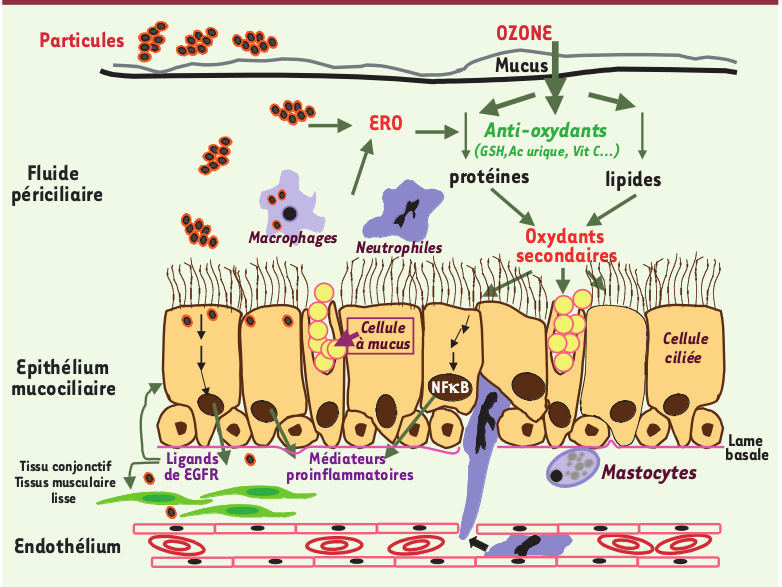
\includegraphics[width=0.8\linewidth]{chapter01/OxydativeMechanism_BaezaMorano2007.png}
    \caption{Mécanismes de toxicité de l’ozone et des particules atmosphériques dans les voies
    aériennes. Crédit : \cite[figure 1]{baezaPollution2007}}%
    \label{fig:mecanisme_oxydation}
\end{figure}

Afin de répondre à cette problématique de métrique sanitaire des PM, il a été proposé
par~\cite{zielinskiModeling1999} et \cite{choRedox2005} une nouvelle mesure, intégratrice
des propriétés physico-chimique des aérosols, sensée être plus proche des impacts
sanitaires occasionnés par les PM : le \textit{potentiel oxydant} (PO, ou
\textit{oxidative potential} (OP)).  Cette nouvelle mesure tente de quantifier les espèces
réactives de l'oxygène présentes ou induites par les aérosols, en utilisant la mise en
contact des aérosols avec un anti-oxydant.  Le suivi de la cinétique de la réaction permet
ainsi d'estimer la réactivité de l'échantillon, prenant en compte non seulement sa chimie,
mais aussi la taille et forme des particules à travers leurs surfaces de réaction et
également les potentiels ``effet cocktail'' lors de la combinaison de différentes espèces
chimiques.

L'avantage de cette méthode acellulaire réside en son faible coût, mais elle aussi est
non-invasive et implémentable en routine en laboratoire, comparativement aux tests
cellulaires nécessitant des prélèvements de tissu et des analyses des protéines marqueuses de
l'inflammation.  Elle permet également une confrontation facilitée aux autres informations
dont l'on dispose sur les PM provenant du même échantillon.

\subsection{Méthodologie de mesure}%
\label{sub:methodologie_de_mesure}

Il n'existe pas à l'heure actuelle de méthodologie standardisée de mesure du potentiel
oxydant. Plusieurs méthodes coexistent et apportent chacune une vision différente du PO.

Il faut noter également que ces méthodes n'ont pas été développées lors de ma thèse mais
s'appuient sur les travaux de \cite{calasPollution2017} et que les échantillons ont été
analysés par les différent·e·s techniciennes et techniciens du plateau analytique
Air-O-Sol de l'IGE.

\subsubsection{Différents agents réactants}%
\label{ssub:differents_agent_reactant}

La mesure du PO se faisant par suivi cinétique de la déplétion d'un anti-oxydant
lorsqu'il est mis au contact des PM, le choix de l'anti-oxydant induit des mesures de PO
différentes. Au cours de cette thèse, 2 mesures différentes sont utilisées conjointement :
le test au dithiothreitol (DTT) et à l'acide ascorbique ou vitamine-A (AA), et sont
explicités dans le chapitre suivant (section~\ref{sub:potentiels_oxydants}).

D'autres méthodes de mesures du PO existent, mais n'ont pas été utilisées au courant de
cette thèse, à savoir :
\begin{description}
    \item[Electron spin résonance ESR] sensé ciblé particulièrement le radical
        \ce{HO^{.}} \autocite{shiHydroxyl2003,shiTemporal2003}
    \item[DCFH]\todo{ref}
    \item[Mélange d'anti-oxydant] Bien que la plupart du temps testé indépendamment, il est
        possible d'estimer un ``PO moyen'' par la mise en contact de différents
        anti-oxydants simultanément (acide ascorbique, glutation et urée par exemple)~\autocite{calasComparison2018}
    \item[todo] \todo{Mesure directe de OH° (mise en place en à l'IGE dans le cadre d'un
        programme financé par le LEFE-CHAT)}
\end{description}

\subsubsection{Un ``meilleur'' test que les autres ?}%
\label{ssub:un_meilleur_test_que_les_autres_}

Les différents tests de PO ne sont pas sensibles aux mêmes espèces chimiques ni même aux même
conditions physico-chimiques. En effet, l'étude de \cite{kunzliComparison2006} sur 20
sites européens présente des corrélations différentes entre le PO mesuré par ESR, AA ou
GSH au regard de la masse des PM et les métaux les constituants.
Ce résultat a été retrouvé depuis par de nombreuses études, et pour le test au DTT et DCFH
également. Par conséquent, cela montre que différents constituants des PM agissent
différemment et à travers des mécanismes oxydatifs divers, capturés par certains tests et
non par d'autres.
Il est donc probable que certaines affections sanitaires soient reliées à un test donné, et
d'autres affections à un autre test. En l'absence de travaux plus approfondis en toxicologie
et épidémiologie, il n'est donc pas possible en l'état actuel des connaissances de trancher
pour ``le meilleur test de PO''.

Par conséquent, les travaux de cette thèse s'emploient à étudier conjointement le PO
mesuré par DTT et par acide ascorbique.


\subsection{Attribution du PO aux sources d'émissions des PM}%
\label{sub:attribution_du_po_aux_sources_d_émissions_des_pm}

Les mesures de PO étant fastidieuses, il a fallu attendre la mise en place de technique
de semi-automatisation pour obtenir des séries temporelles de mesure de ``longue durée''. Les récents
travaux de \cite{fangSemiautomated2015}, parallèlement aux travaux de
\cite{calasPollution2017}, ont permis ce pas technique, permettant l'analyse accrue de
prélèvements et les premières séries annuelles de mesure des PO, conjointement avec
l'analyse de la chimie des filtres prélevés.

\subsubsection{Corrélation PO -- chimie}%
\label{ssub:corrélation_po_chimie}

Les liens entre la chimie des particules et les résultats de PO s'est dans un premier temps focalisé
sur la simple corrélation univariée. Ainsi, le Cu présente de fortes corrélations
avec le \PODTT{} et \POAA, de même que le carbone organique, etc. Seulement, la simple
corrélation montre également une forte corrélation entre le \PODTT{} et le \ce{NO3-},
pourtant inerte en termes d'oxydo-réduction.
En effet, une corrélation n'implique pas une causalité, et cette corrélation ne résulte
que d'une co-correlation entre le \ce{NO3-} et d'autres espèces, rédox-actives.

\todo{parler des quinones, add ref, etc}


\subsubsection{Sources de PM et de PO}%
\label{ssub:sources_de_pm_et_de_po}

% Enfin, il n'est pas possible de mesurer l'ensemble des espèces chimiques constituant les
% PM. Devant cette foultitude, il paraît donc illusoire de pouvoir attribuer un PO
% intrinsèque à chacune des espèces chimique.
% En revanche, si l'on bénéficie d'un nombre suffisant d'échantillon, il est alors possible
% d'estimer les sources ou facteurs d'émissions (voir
% section~\ref{sec:source_apportionment_of_pm}). Ce faisant, la vision par ``source'' plutôt
% que par ``espèce'' permet une agrégation de l'information, en regroupant un ensemble
% d'espèce, mesurée ou non, provenant d'une même source d'émission, en une seule variable.
% Ainsi, il est possible d'attribuer un PO à une source donnée, sans pour autant avoir
% besoin de savoir quelles sont les espèces chimiques émises par cette source qui
% contribuent au PO.
% De plus, en termes de régulation, la vision par source est davantage pertinente car permet
% potentiellement une action politique plus rapide que s'il s'agissait de cibler une espèce
% chimique particulière.

Il est aussi possible de chercher à attribuer un PO non pas à une espèce chimique mais à
une source spécifique.
\todo{work in progress}

\paragraph{Mesures directes à l'émission}%
\label{par:mesures_directes_à_l_émission}

\todo{parler de l'étude de Lucille dans sa thèse. Citer un projet possible avec l'INERIS,
en cours d'écriture. }

\paragraph{Études sur sites et en air ambiant}%
\label{par:études_sur_sites_et_en_air_ambiant}

Les premières études de ce type sont celles de
\cite{vermaReactive2014,batesReactive2015,fangOxidative2016}, et utilisent 2 approches
différentes :
\begin{enumerate}
    \item Incorporation de PO comme variable d'entrée d'une étude PMF au même titre qu'une
        autre espèce chimique ;
    \item Analyse de sources via le CMB (sans PO), puis régression linéaire entre les
        sources de PM ainsi déduites et le PO.
\end{enumerate}
Bien que de façon inhérente aux différences entre PMF et CMB les sources retrouvées ne
sont pas exactement les mêmes, les auteurs montrent que la combustion de biomasse est la source
principale de \PODTTv, suivie de près par le trafic routier (ensemble des émissions
véhiculaires et de la remise en suspension de poussière de route), puis le sulfate
d'ammonium et enfin un facteur de composés organiques secondaires solubles.
Concernant le \POAAv, \cite{fangOxidative2016} (voir
figure~\ref{fig:chapter01/fangOxidative2016-fig4}) estiment à autour de \SI{45}{\percent} la
contribution des émissions véhiculaires et à environ \SI{50}{\percent} la contribution de
facteur secondaire (organique et inorganique).

\begin{figure}[ht]
    \centering
    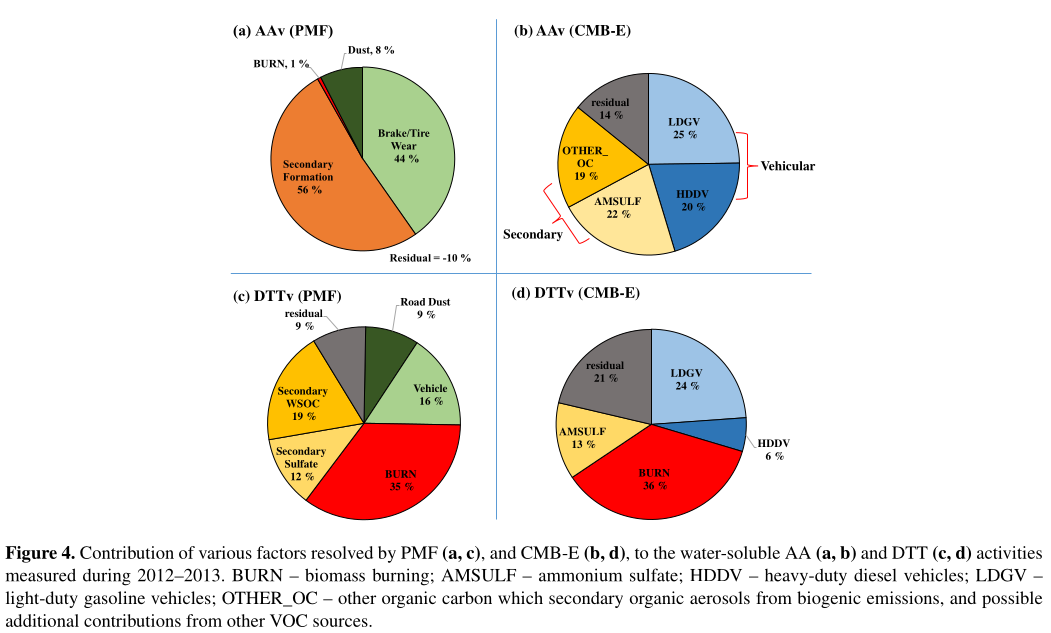
\includegraphics[width=1.0\linewidth]{chapter01/fangOxidative2016-fig4.png}
    \caption{Contribution des sources de PM aux \POAAv{} et \PODTTv{} par l'étude de
    \cite{fangOxidative2016} portant sur un ensemble de 238 échantillons sur 3 sites
        distincts à Atlanta, US, pendant l'année 2012-2013.}%
    \label{fig:chapter01/fangOxidative2016-fig4}
\end{figure}

Lors du commencement de ma thèse, seules ces études étaient, à ma connaissance,
disponibles dans la littérature concernant l'attribution des sources de PM aux potentiels
oxydants.  Depuis, de nouvelles études ont été publiées, et seront discutées dans le
chapitre~\ref{cha:estimation_des_sources_de_PO}.


\section{Objectifs de cette thèse}%
\label{sec:positionnement_de_cette_thèse}

Ma thèse s'inscrit donc dans cette double problématique de l'identification et de la
quantification des contributions massiques des différentes sources d'émission de PM en air
extérieur, mais aussi de leurs contributions au nouvel indicateur qu'est le potentiel
oxydant.

Premièrement, il s'agit d'améliorer l'outil de déconvolution des sources de PM
\textit{Positive Matrix Factorization}, non pas par de nouveaux développements mathématiques de
résolution de l'équation de conservation des masses, mais par l'élaboration d'une
expertise dans les différentes paramétrisations de ce modèle, dans son entraînement et
dans la critique de ses résultats. Notamment, la question de la présence de l'ensemble
des sources majoritaires se posera dans le
chapitre~\ref{cha:approfondissement_des_connaissances_des_sources_des_pm}, à travers
l'implémentation de nouveaux traceurs chimiques ou isotopiques.
Également, les incertitudes des solutions PMF ne sont quasiment jamais explicitées alors
que c'est une question centrale qui intéressent d'autant plus les décideurs publics. Mes
travaux tenteront donc de quantifier les incertitudes des contributions des sources aux
espèces mesurées.
Aussi, pour pouvoir généraliser des études PMF à différents sites, il faut auparavant
non seulement s'assurer que les méthodes sont similaires entre les études (mêmes espèces
chimiques…) mais aussi estimer objectivement la similitude de deux facteurs que l'on estime provenir
de la même source d'émission, c'est-à-dire comparer les solutions entre elles.

\todo{Blabla PO}

\subsection{Questionnement et plan de la thèse}%
\label{sub:plan_de_la_thèse}

Ainsi, mes recherches tenteront de répondre aux questions suivantes :

\begin{itemize}
    \item Comment obtenir des contributions et profils de sources reflétant au mieux les
        processus d'émissions et de transformation dans l'atmosphère ?
        (Chapitre~\ref{cha:approfondissement_des_connaissances_des_sources_des_pm})
    \item Est-il possible de diminuer la subjectivité de l'expérimentateur dans ces
        études d'attribution des sources ?
        (Chapitre~\ref{cha:approfondissement_des_connaissances_des_sources_des_pm})
    \item Comment comparer efficacement 2 profils attribués à la même source, à
        différents sites de prélèvement et différentes années de mesure ?
        (Chapitre~\ref{cha:approfondissement_des_connaissances_des_sources_des_pm})
    \item Comment remonter à la contribution des sources de PO une fois les sources
        d'émissions de PM identifiées ?
        (Chapitre~\ref{cha:estimation_des_sources_de_PO})
    \item Les sources contribuants au potentiel oxydant sont-elles les mêmes que celles
        contribuant à la masse des PM ?
        (Chapitre~\ref{cha:estimation_des_sources_de_PO})
    \item Est-ce que les valeurs PO des sources des PM sont les mêmes à large échelle spatiale ou
        sont-elles dépendantes du lieu considéré ?
        (Chapitre~\ref{cha:estimation_des_sources_de_PO})
    \item Est-il possible, à terme, d'obtenir une prévision du PO intégré à la prévision
        de la qualité de l'air, complémentairement à la concentration massique ?
        (Chapitre~\ref{cha:estimation_des_sources_de_PO} et~\ref{cha:travaux_futur})
\end{itemize}

Ces différentes questions seront abordées entre autres avec la présentation des résultats de
recherches déjà publiés dans 7 articles scientifiques auxquels j'ai contribué (dont 2 
en premier auteur) ainsi que par des travaux en cours de publication (6, dont 2 en premier auteur).
La liste complète de ces travaux est fournie en annexe~\ref{annexe:CV} et s'appuie sur un
grand nombre de programmes de recherche
(voir~\ref{annexe:programmes_ayant_financés_la_thèses}). Les articles en
premier auteur sont reproduits in extenso.


\chapter{Matériel et méthode}
\label{cha:materiel_et_methode}
\PartialToc
\clearpage

\section{Stratégie générale du groupe CHIANTI}%
\label{sec:stratégie_générale_du_groupe_chianti}

\section{Methodologie de prélèvement et d'analyse}%
\label{sec:methodologie_de_prélèvement_et_d_analyse}

\section{Profile de source des solutions PMF}%
\label{sec:profile_de_source_des_solutions_pmf}

\section{Harmonisation et gestion de base de donnée}%
\label{sec:harmonisation_et_gestion_de_base_de_donnée}



\chapter{Faire de bonnes PMF}
\label{cha:bonnes_PMF}
\PartialToc
\clearpage

\section{Amélioration des solutions PMF par ajout de traceurs spécifiques}%
\label{sec:amélioration_des_solutions_pmf}

\subsection{Isotopie}%
\label{sub:isotopie}

\subsection{Émission biogénique primaire}%
\label{sub:émission_biogénique_primaire}

\subsection{Processus secondaires}%
\label{sub:processus_secondaires}

\section{Confrontation des solutions PMF}%
\label{sec:confrontation_des_solutions_pmf}

\subsection{Incertitudes associées}%
\label{sub:incertitudes_associées}

\subsection{Comparabilité des solutions}%
\label{sub:comparabilité_des_solutions}

\section{SOURCES}%
\label{sec:sources}




\chapter{Approfondissement des connaissances des sources des PM}%
\label{cha:approfondissement_des_connaissances_des_sources_des_pm}
\PartialToc
\clearpage
% \section*{Introduction}%
\label{sec:introduction}
\addcontentsline{toc}{section}{Introduction}


Les travaux présentés dans ce chapitre ont été menés afin d'approfondir les connaissances
des processus d'émissions de différents composés des PM. En effet, le modèle PMF utilisé
pour tracer l'origine des sources d'aérosol nécessite une base de connaissance préalable à
son utilisation car comme nous l'avons vu, plusieurs paramètres doivent être choisis par
l'expérimentateur, notamment les variables servant d'entrainement au modèle.

Un modèle étant nécessairement une représentation simplifiée de la réalité, il convient de
trouver le bon équilibre entre un modèle trop complexe, qui serait difficilement
interprétable, et un modèle trop simple, qui n'apporterait pas de nouvelles informations.
Le cas de la PMF, et le \textit{machine learning} en général, n'échappe pas à cette règle.
Il faut en effet choisir soigneusement les variables d'entrée du modèle pour lui permettre
d'extraire des informations géochimiquement pertinentes d'un ensemble de donnée. Cela se
traduit par la détermination d'espèce traceuse de processus d'émissions ou de
transformations dans l'atmosphère, puis de leur utilisation conjointe dans le modèle PMF,
permettant alors d'isoler de nouveaux facteurs et de raffiner la contribution des autres
espèces aux facteurs restants.

Aussi, un modèle procède toujours à une étape de validation. Dans notre cas, nous n'avons
pas de référence pouvant servir de témoin positif. Nous pouvons cependant nous servir de
2 procédés : 1) la confrontations à d'autres méthodes de \textit{sources-apportionment},
indépendantes de la PMF (carbone 14 (\textcite{bonvalotEstimating2016} et
\textcite{chevrierChauffage2016}), Aethalometre, etc) ou 2) estimer la fiabilité des
résultats PMF par cohérence géophysique, par exemple en retrouvant l'origine géographique
des sources d'émissions.

Les travaux de cette thèse ont ainsi conduit à différents développements ou applications
méthodologiques et techniques.
\begin{enumerate}
    \item Nous verrons dans un premier temps que l'origine géographique des masses d'air
        par méthode PSCF a permis de consolider les solutions obtenues par méthodologie
        PMF, mais a également apportée une vision nouvelle de la provenance du MSA,
        supposé jusqu'alors d'origine exclusivement marine~\autocite{gollyOrganic2019}.
    \item Dans un second temps, nous expliquerons en quoi le recensement et
        l'harmonisation de la base de donnée de filtre de prélèvement ambiant a été
        utilisé afin de généraliser des observations à un ensemble de 28 sites de
        mesures et a conduit à la quantification des processus d'émissions biogéniques
        primaires~\autocite{samakePolyols2019,samakeArabitol2019}.
    \item Enfin, nous présenterons un travail en cours sur la variabilité fine échelle
        des sources de PM et l'importances des facteurs d'oxydations secondaires,
        identifiés par l'ajout de nouveaux traceurs organiques dans la
        PMF~\autocite{borlazaSourceinprep}.
\end{enumerate}
\todo{Et INACS dans tout ca ?}


\section{Provenance géographique des composés chimiques et facteurs}%
\label{sec:provenance_géographique_des_composés_chimiques_et_facteurs}

Pour déterminer l'origine des sources des composés chimiques retrouvé à un site récepteur,
il est possible de retracer sa provenance géographique. Nous verrons d'abord le cas simple
de la rose des polluants, avant d'expliciter plus en avant la méthode PSCF.

\subsection{Cas simple : la rose des polluants}%
\label{sub:cas_simple_la_rose_des_polluants}

L'un des moyens les plus simples pour cela est de coupler des mesures de direction et
vitesse de vent et d'établir une rose des polluants. J'ai pu utiliser ce procédé à des
fins exploratoires lors de ma thèse, ce qui m'a conduit à contribuer au développement du
package python
\href{https://github.com/python-windrose/windrose/}{windrose}~\autocite{scls19frPythonwindrose2019}.
Cependant, cette méthode n'est utile que pour la détermination de source proche du site
récepteur car dès lors que l'on s'en éloigne, l'orientation et vitesse des vents varient
et l'hypothèse de déplacement uniforme de la masse d'air est invalidée.  Or, il est
courant que les aérosols proviennent de sources non locales, limitant l'utilisabilité de
cette méthode.

En revanche, il est possible d'utiliser les rétrotrajectoires complètes des masses d'air
pour remonter aux sources géographiques potentielles et également de coupler ces
trajectoires à des informations physico-chimiques comme la concentration en polluants
observés sur le site récepteur, la présence de pluie déposant les aérosols par dépôt
humide ou encore la hauteur de la masse d'air.

\subsection{Prendre en compte l'histoire de la masse d'air : PSCF}%
\label{sub:prendre_en_compte_l_histoire_de_la_masse_d_air_PSCF}

\subsubsection{Méthodologie}%
\label{ssub:méthodologie}

L'une des méthodes les plus largement utilisée dans la littérature est la \textit{Potential
source contribution function} (PSCF), permettant de combiner des ensembles de trajectoires à
des modèles récepteurs. Le principe consiste à calculer les rétrotrajectoires d'un site
récepteur donné et d'associer à chacune d'elle la concentration du polluant ou de la
source considéré le jour de son passage au niveau du site récepteur. En discrétisant les
trajectoires en 1 point toutes les X minutes ou heures et en appliquant une grille
régionale, il est alors possible de dénombrer combien de rétrotrajectoires sont passés par
chacune des grilles.  Le ratio du nombre de trajectoire associée à une forte concentration
aux coordonnées $i$, $j$, noté $m_{ij}$, par le nombre total de trajectoire étant passé
par ces coordonnés notées $n_{ij}$, nous donne une probabilité de provenance géographique
de ce composé ou source pour les coordonnées $i$, $j$, noté $PSCF_{ij}$ :
\begin{align}
    \label{eq:PSCF}
    PSCF_{ij} &= \frac{m_{ij}}{n_{ij}}.
\end{align}

Des améliorations ont été apportées à cette méthode afin de prendre en compte les cellules
ayant un faible pourcentage de passage de rétrotrajectoires, augmentant artificiellement
le ratio $\frac{M}{N}$. Une manière de contrebalancer ce biais et d'ajouter une fonction
poids, dépendant de la fréquence de passage des rétrotrajectoires sur chacune des
cellules. Dans la figure~\ref{fig:chapter02/PSCF_method}, illustrant la PSCF, on voit que
la cellule où 2 rétrotrajectoires sont passés se voit attribuer la même probabilité que
celles avoisinantes, où seule une rétrotrajectoire a résidé. Or, il serait plus pertinent
d'avoir une probabilité plus forte pour cette cellule, indiquant que chaque
rétrotrajectoire ayant résidé à ces coordonnées est riche du composé suivit.  Différentes
fonctions poids existent, le plus souvent présentant différents seuils en fonction du
nombre de rétrotrajectoires par cellule~\autocite{bressiSources2014,petitSources2019}.

Aussi, pour avoir une représentativité statistique suffisante des sources potentielles, il
est nécessaire de calculer un grand nombre de rétrotajectoire, correspondant à chacun des
jours de prélèvement sur le site récepteur.


\begin{figure}[ht]
    \centering
    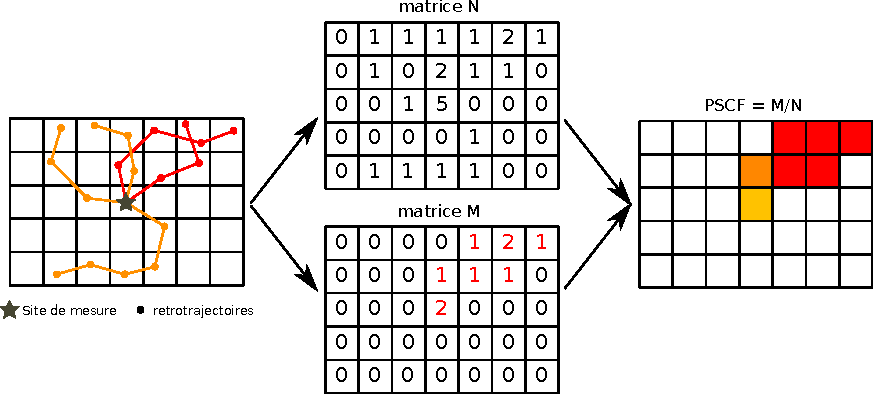
\includegraphics[width=0.9\linewidth]{chapter02/PSCF_method.pdf}
    \caption{Illustration de la méthode PSCF : les rétrotrajectoires depuis le site de
        mesure sont calculées, celles associées à une concentration seuil sont
        représentées en rouge, les autres en orange. Les matrices N et M s'obtiennent par
        simple décompte du nombre de rétrotrajectoires passés dans chaque cellule de
        taille prédéfinies, puis le ratio nous donne une estimation de l'origine
    géographique, représentée ici terme d'intensité de rouge.}%
    \label{fig:chapter02/PSCF_method}
\end{figure}

\subsubsection{Automatisation et simplification : pyPSCF}%
\label{ssub:automatisation_et_simplification_pypscf}

Ces étapes fastidieuses de calcul des rétrotrajectoires et de PSCF ont été automatisés
dans un paquet python, pyPSCF\footnote{Dépot git pyPSCF:
\url{https://gricad-gitlab.univ-grenoble-alpes.fr/webersa/pyPSCF}}, permettant le
traitement d'un grand nombre de rétrotrajectoire en utilisant le modèle lagrangian
HYSPLIT et calculant de manière facilité une PSCF en un site donné, en variant notamment
les différents paramètres succeptibles d'influencer le modèle.

\subsection{Application : Importance et origine géographique du MSA ? (Golly et al. 2019)}%
\label{sub:origine_terrestre_ou_marine_du_msa_}

Comme expliqué précemment, une part importante des aérosols provient de sources
secondaires, c'est-à-dire du vieillissement et des réactions dans l'atmosphère. Une part
importante de ces aérosols secondaires sont d'origines organiques. Les travaux
de~\textcite{gollyOrganic2019}, auxquels j'ai pris part, s'attachent notamment à la
quantification de cette matière organique secondaire, sur 5 sites ruraux en France
pendant l'année 2013, par la mesure de deux espèces issues de processus secondaires : le
MSA et l'oxalate.  Nous avons pu montrer que le MSA, considéré comme provenant de
l'oxydation du DMS, peut contribuer jusqu'à 10 à 20\% de l'OC en période chaude,
indiquant une forte proportion d'aérosols organiques secondaires durant l'été. Mais
surtout, le MSA est considéré comme provenant des émissions de DMS du phytoplanction
marin, au point qu'il est proposé comme méthode de séparation entre le sulfate d'origine
marine et ses autres provenances.

En conduisant une analyses PSCF sur les 25\% des jours les plus fortement chargés en MSA,
nous avons pu confirmer l'importance marine de ce composé, mais également montrer qu'une
part non négligeable semble provenir d'environnement terrigène (voir
figure~\ref{fig:chapter02/golly_PSCF_MSA}), confortant les études suggérants des
processus d'émissions du MSA par des sources biologiques
terrestres~\autocite{bozzettiArgon2017}, pouvant provenir des forêts ou des
sols~\autocite{jardineDimethyl2015,miyazakiSeasonal2012}.

L'une des implications directes de ces travaux résulte en l'ajout systématique du MSA
comme variable d'entrée des études PMF, quelque soit leur localisation. En effet, le
signal du MSA est clairement distinct des autres espèces chimiques mesurées et représente
également une part important de la matière organique. Cette espèce est donc a minima
traceuse de processus secondaires présent sur l'ensemble de l'europe occidental.

\begin{figure}[ht]
    \centering
    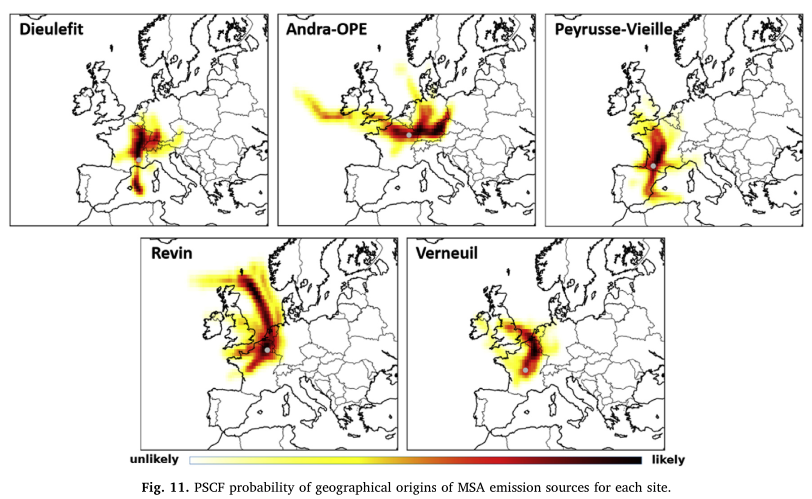
\includegraphics[width=0.9\linewidth]{chapter02/golly_PSCF_MSA.png}
    \caption{Probabilité de l'origine géographique du MSA, issue de l'article
        de~\textcite{gollyOrganic2019}. Bien que l'on retrouve l'origine marine du MSA,
        les sites de Dieulefit, OPE ou Peyrusse-Vieille indiquent également une forte
        probabilité d'origine terrestre de ce composé.}%
    \label{fig:chapter02/golly_PSCF_MSA}
\end{figure}

\subsection{Application 2 : Validation des solutions PMF}%
\label{sub:application_2_validation_des_solutions_pmf}

Une autre utilisation de la PSCF consite à croiser les informations issues de la PSCF et
des PMF.
En effet, il n'existe pas de moyen simple de valider le sens géochimique d'une solution
PMF autrement que l'expertise et les connaissances de l'utilisateur.
Une fois une solution obtenu, il est possible de conduire une étude PSCF sur les
différents facteurs identifiés par la PMF. Ainsi, on s'attend à ce que le facteur
\textit{sel de mer} provienne géographiquement d'un océan ou d'une mer. De même la
\textit{combustion de biomasse domestique} ne devrait pas pointer d'emplacement
particulier puisqu'il s'agit d'une source diffuse.

\todo{Exemple de l'OPE : sel de mer et combustion de biomass}


\section{Généralisation d'observations}%
\label{sec:généralisation_dobservations}

\subsection{Mise en place d'une base de donnée harmonisée}%
\label{sub:mise_en_place_d_une_base_de_donnée_harmonisée}

\subsection{Application : Importance des émissions primaires biogéniques (Samaké et al.
2019)}%

\label{sub:application_importance_des_émissions_primaires_biogéniques_samaké_et_al_2019_}


\section{De nouveaux traceurs secondaires pour les PMF ?}%
\label{sec:amélioration_des_solutions_pmf_grâce_à_de_nouveaux_traceurs_organiques}

\subsection{Problématique}%
\label{sub:problématique}

\subsection{Ajout des acides organiques comme traceur du SOA ? (Borlaza et al. in prep)}%
\label{sub:ajout_des_acides_organiques_comme_traceur_du_soa_borlaza_et_al_in_prep_}




\printbibliography[segment=\therefsegment,heading=subbibliography]



\chapter{Développent méthodologique d'attribution des sources de PM}
\label{cha:developpement_methodologique_dattribution_des_sources_de_PM}
\PartialToc
\clearpage
% % vim: spelllang=en

\begin{otherlanguage}{english}
\section{Introduction} 

Particulate matter (PM) in ambient air is known to have significant impacts on the Earth
climate~\autocite{stockerClimate2013}. It is also recognized to induce adverse human
health effects. A~growing number of studies are notably confirming its influence on the
occurrence of respiratory and cerebrovascular diseases, as~well as heart attacks and other
cardiovascular issues ~\autocite{kellyLinking2015,lippmanNational2013}. The~implementation
of action plans to effectively improve air quality relies on sound knowledge of their
origins. However, the~scientific community and public authorities are still facing issues
to clearly identify efficient mitigation policies. This is notably due to the multiplicity
of PM emission sources and the complexity of their (trans)-formation,   from both primary
and secondary processes in the~atmosphere. 

Several methodologies have been developed and used in the last decades for PM source
apportionment purposes. Among~them, receptor-oriented models (RMs) have been widely used
to discriminate the main PM fractions based on the investigation of co-variations of
chemical species measured at a given location, which  should include specific
tracers~\autocite{srivastavaSpeciation2018,karagulianContributions2015,belisCritical2013,vianaSource2008}.
In~particular, positive matrix factorization (PMF) relies on two data matrices that
contain the concentrations of measured particulate species and their corresponding
uncertainties, respectively. One of the main features of the PMF results is their
quantitative nature, allowing to evaluate the contributions as well as the chemical
composition of the main PM fractions~\autocite{paateroLeast1997, paateroPositive1994}.
These PM fractions may correspond to primary aerosols emitted by a given type of emission
sources, to a group of chemical species formed through similar and/or concomitant
secondary processes in the atmosphere, or~to a mixing of both primary and secondary
aerosols. Their chemical profiles are then used for their identification and labeling,
based on the current knowledge of emission chemical footprints and of atmospheric
secondary processes. The~availability of well-known real-world PM chemical profiles is
essential to validate the attribution of factors obtained from the PMF analyses.
The~scarcity of local source profiles often represents a challenge for RMs in terms of
both the identification of sources and the comparability between~studies.

In this context, libraries gathering various PM chemical source profiles obtained from
previous studies are of great interest for the scientific community. The~SPECIATE database
has been made available by the US EPA since 1988~\autocite{simonDevelopment2010}, now
containing over 3000 local source profiles. More recently, a~similar effort has been
conducted in Europe, leading to the SPECIEUROPE database as described
by~\textcite{pernigottiSPECIEUROPE2016}.  This database could be implemented thanks to
various recent PMF studies, such as those described
in~\textcite{vianaSource2008,belisCritical2013,karagulianContributions2015,mooibroekPM102016,perronePM2016}
and reference therein.  However, the~robustness of these source profiles needs to be
assessed more deeply and outputs from additional source apportionment studies are still
needed to increase the European coverage and to document various aerosol fractions and/or
geographical areas.  In particular, a~very limited number of comprehensive PM$_{2.5}$
and/or \PM{} source apportionment studies were conducted in France before
2012~\autocite{elhaddadPrimary2011,elhaddadInsights2011,bressiSources2014,wakedSource2014}.
To~fill this gap, the~research community along with regional monitoring networks put
common efforts into extensive filter samplings, off-line chemical analyses and statistical
data treatments for numerous French locations~\autocite{amodeoProgrammes2017}.  Moreover,
the~SOURCES project has been set-up to deliver a comprehensive overview of these
filter-based source apportionment studies achieved in France for the 2012--2016
period~\autocite{favezEtat2017}.

Here, we present some of the main results obtained within this SOURCES project, based on
the outputs of PMF analyses conducted for 15 datasets corresponding to various sampling
sites distributed all over France. An~innovative aspect of this study is that PMF analyses
have been achieved in a harmonized way, allowing for a proper comparison of the results.
Furthermore, all the outcomes of the project, including time-series and source profiles
along with their corresponding uncertainties, have been made available through a website
interface, proposed as Supplementary Material for this article,
at~\url{http://pmsources.u-ga.fr}. This methodology offers a unique opportunity to compare
main PM factor's contributions and chemical footprints at a national scale. The~results
were first investigated for their representativity and homogeneity at a national scale,
also including a presentation of the variability and the seasonality of their
contributions to the \PM{} mass. The~large set of chemical profiles of the PM sources
obtained in this work also allows for a discussion on their similarities and uncertainties
using different metrics, including the bootstrap (BS) and displacement (DISP)
analysis~\autocite{paateroMethods2014}. Assessing the stability of chemical profiles
across a comparable set of studies is an important aspect in the perspective of using
these profiles as benchmarks for future~works.

\section{Materials and~Methods}%NOTE: Please confirm all titles are capitalized correctly.
\label{sec:materials_and_methods}

\subsection{PM Sampling~Sites}%
\label{sub:pm_sampling_sites}

Figure~\ref{fig:fig1} shows the geographical location of the 15 sampling sites for which
comparable datasets (in terms of number of samples, investigated period and \PM{} chemical
speciation data) were made available for the present study through the SOURCES project.
Table~\ref{tab:tab1} summarizes the characteristics of these sites. Most of them
correspond to urban background stations and are distributed throughout France, including
two Alpine cities (classified herewith as ``Urban valley'').  Other site typologies could
also be investigated, with~two urban traffic sites, one industrial, as~well as one EMEP
(European Monitoring and Evaluation Programme, \url{https://www.emep.int/)} rural
background~station. 

At each site, \PM{} concentrations were monitored using automated analyzers, in~accordance
with recommendations of EN~16450:2017~\autocite{cenAmbient2017b}, and daily (\SI{24}{h})
filter samples were collected every third day by employees of the corresponding regional
air quality monitoring network. Samplings were achieved on pre-heated quartz fiber filters
using high-volume sampler (DA80, Digitel), following EN~12341:2014
procedures~\autocite{cenAmbient2014}. Off-line chemical analyses performed on these
filters are fully described in the Figure~SI-1 of the Supplementary Material. Briefly,
the~elemental and organic carbon fractions (EC and OC) were measured via thermo-optical
analysis (Sunset Lab. Analyzer~\autocite{birchElemental1996}) using the EUSAAR-2
protocol~\autocite{cavalliStandardised2010,cenAmbient2017a}.  Major water-soluble
inorganic contents (\ce{Cl-}, \ce{NO3^-}, \ce{SO4^2-}, \ce{NH4+}, \ce{Na+}, \ce{K+},
\ce{Mg^2+}, and \ce{Ca^2+}) and methanelsulfonic acid (MSA) were determined using ion
chromatography~\autocite{jaffrezoSeasonal2005,cenAmbient2017a}). Many metals or trace
elements (e.g., Al, Ca, Fe, K, As, Ba, Cd, Co, Cu, La, Mn, Mo, Ni, Pb, Rb, Sb, Sr, V, and
Zn) were measured by ICP-AES or
ICP-MS~\autocite{allemanPM102010,mbengueSizedistributed2014,cenAmbient2005}.  Finally,
various anhydrosugars (including levoglucosan, mannosan, arabitol, sorbitol, and~mannitol)
were analyzed using High Performance Liquid Chromatography followed by pulsed amperometric
detection (HPLC-PAD)~\autocite{wakedSource2014}.

\begin{figure}[ht]
    \centering
    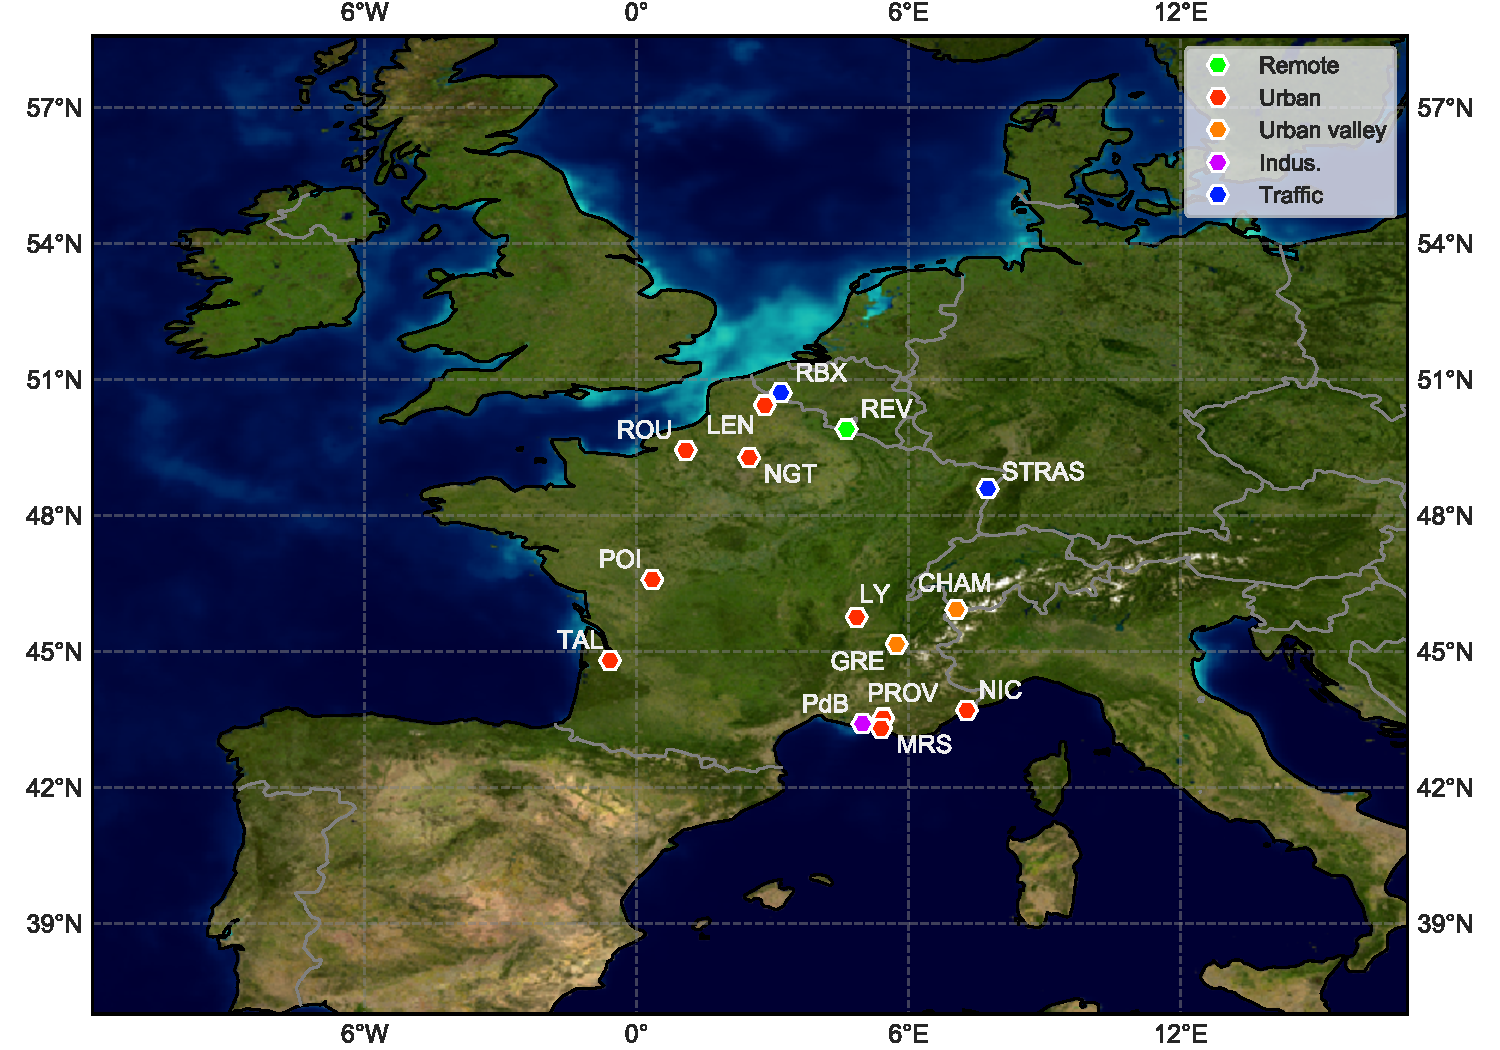
\includegraphics[width=0.9\linewidth]{chapter03/fig1.pdf}
    \caption{
        Map showing he geographical location of the 15 selected sites. Color
        codes denote the typology of the site:  green, remote; red, urban;
        orange, urban valley; magenta, industrial; blue, traffic.
    }
    \label{fig:fig1}
\end{figure}

\begin{sidewaystable}
    \centering
    \caption{Characteristics of the 15 PM sampling sites investigated in the present~study.}
    \label{tab:tab1}
    % \tablesize{\footnotesize}
    \begin{tabular}{lcp{0.11\textwidth}cccp{0.15\textwidth}}
        \toprule
        \textbf{Sampling Site}    & \textbf{Code} & \textbf{Coordinates} & E\textbf{levation}                                  & \textbf{Period }                           & \textbf{N samples} & \textbf{Typology}\\
        \midrule
        Revin            & REV  & \ang{49;55;00.00}N\newline\ang{4;38;29.00}E & \SI{395}{m} & 02 Jan 2013$\rightarrow$01 Jun 2014 & 168       & remote\\%NOTE: Please confirm all dates are in the format DD Month YYYY
        Bordeaux-Talence & TAL  & \ang{44;48; 2.01}N\newline\ang{0;35;17.01}W & \SI{ 20}{m} & 02 Feb 2012$\rightarrow$07 Apr 2013 & 154       & urban background\\
        Lyon             & LY   & \ang{45;45;27.82}N\newline\ang{4;51;15.15}E & \SI{160}{m} & 03 Jan 2012$\rightarrow$31 Dec 2012 & 115       & urban background\\
        Poitiers         & POI  & \ang{46;34;48.80}N\newline\ang{0;20;25.34}E & \SI{106}{m} & 16 Nov 2014$\rightarrow$29 Dec 2015 & 110       & urban background\\
        Nice             & NIC  & \ang{43;42; 7.48}N\newline\ang{7;17;10.53}E & \SI{  1}{m} & 04 Jun 2014$\rightarrow$29 Jun 2016 & 184       & urban background\\
        Marseille        & MRS  & \ang{43;18;18.84}N\newline\ang{5;23;40.89}E & \SI{ 64}{m} & 11 Jan 2015$\rightarrow$27 Jun 2016 & 102       & urban background\\
        Aix-en-Provence  & PROV & \ang{43;31;49.04}N\newline\ang{5;26;29.00}E & \SI{180}{m} & 18 Jul 2013$\rightarrow$13 Jul 2014 & 56        & urban background\\
        Nogent sur Oise  & NGT  & \ang{49;16;35.00}N\newline\ang{2;28;56.00}E & \SI{ 28}{m} & 02 Jan 2013$\rightarrow$02 Jun 2014 & 155       & urban background\\
        Rouen            & ROU  & \ang{49;25;41.40}N\newline\ang{1;03;29.10}E & \SI{  6}{m} & 02 Jan 2013$\rightarrow$01 Jun 2014 & 162       & urban background\\
        Lens             & LEN  & \ang{50;26;12.60}N\newline\ang{2;49;36.70}E & \SI{ 47}{m} & 02 Jan 2013$\rightarrow$01 Jun 2014 & 167       & urban background\\
        Grenoble         & GRE  & \ang{45;09;42.84}N\newline\ang{5;44;08.15}E & \SI{214}{m} & 02 Jan 2013$\rightarrow$29 Dec 2014 & 240       & urban background\newline\& alpine valley\\
        Chamonix         & CHAM & \ang{45;55;21.00}N\newline\ang{6;52;12.00}E & \SI{1038}{m}& 02 Nov 2013$\rightarrow$31 Oct 2014 & 115       & urban background\newline\& alpine valley\\
        Port de Bouc     & PdB  & \ang{43;24;07.99}N\newline\ang{4;58;55.99}E & \SI{  1}{m} & 01 Jun 2014$\rightarrow$27 Jun 2016 & 185       & urban background\newline\& industrial\\
        Roubaix          & RBX  & \ang{50;42;23.60}N\newline\ang{3;10;50.50}E & \SI{ 10}{m} & 20 Feb 2013$\rightarrow$26 May 2014 & 157       & urban traffic\\
        Strasbourg       & STG  & \ang{48;34;24.25}N\newline\ang{7;45;07.60}E & \SI{139}{m} & 02 Apr 2013$\rightarrow$08 Apr 2014 & 78        & urban traffic\\
        \bottomrule
    \end{tabular}
\end{sidewaystable}


\subsection{PMF~Methodology}%
\label{sub:pmf_methodology}

\subsubsection{PMF~Model}%
\label{ssub:pmf_model}

The U.S. Environmental Protection Agency (US-EPA) PMF5.0 software~\autocite{norrisEPA2014}
was used in the present study to achieve the PM source apportionment. Similar to other RM
approaches, PMF aims at solving the mass conservation between the measured species
concentrations and source emissions as a linear combination of factors $p$, species
profile $f$ of each source,  and the~amount of mass $g$ contributed to each individual
sample, following Equation~(\ref{eq:PMF}):

\begin{equation}
    \label{eq:PMF}
    X_{ij} = \left( \sum_p g_{ip} \times f_{pj} \right) + e_{ij}
\end{equation}

where $X_{ij}$ represents the measured data for species $j$ in sample $i$, and~$e_{ij}$ is
the residual of each sample and species not fitted by the model.  Detailed information on
the PMF methodology can be found elsewhere
~\autocite{paateroPositive1994,paateroLeast1997}. Briefly, a~multivariate factor analysis
was applied to decompose the matrix of the chemical dataset into two matrices: factor
contributions ($G$) and factor profiles ($F$), each factor to be ascribed to a specific
aerosol fraction (i.e., factor), that may be attributed to a source.  It is based on a
weighted least square fit, where the weights are derived from the analytical uncertainty,
and~provides the optimal solution by minimizing the function $Q$, given by
Equation~(\ref{eq:PMFQ}):

\begin{equation}
    \label{eq:PMFQ}
    Q = \sum_i \sum_j \left(\frac{e_{ij}}{\sigma_{ij}}\right)^2
\end{equation}

where $\sigma_{ij}$ represents the measurement uncertainty of each data~point.

\subsubsection{Input Variable and~Uncertainties}%
\label{ssub:input_variable_and_uncertainties}

Selection of the input variables was done based on the percentage of values above
detection limit (DL) (using \SI{60}{\percent} as a minimum threshold), and~the value of
the signal-to-noise ratio (S/N) for each species~\autocite{paateroDiscarding2003}.
Table~\ref{tab:input_var} presents the PMF input variables selected for this work. This
dataset notably includes EC, major ions, molecular organic markers (MSA, levoglucosan, and
mannosan), and~a selection of metals or trace elements. Assuming that they mainly
originate from the same sources---i.e.,~primary biogenic emissions--- sorbitol, arabitol
and mannitol concentrations were summed and labeled as
polyols~\autocite{samakePolyols2019}. Furthermore, \emph{OC*} was determined by
subtracting the carbon concentrations of the specific organic markers to total \emph{OC}
concentrations, so that they are not accounted twice:

\begin{equation}
    OC^* = OC - ([MSA]\times0.12+[polyols]\times0.40+[levoglucosan]\times0.44+[manosan]\times0.44),
\end{equation}

where the coefficient are the carbon mass par unit of~mass.

The different variables were categorized in the model based on their mean signal-to-noise
ratio (S/N) as follows: ``strong'' if $S/N>2$, ``weak'' if $0.2\leq S/N\leq2$, and~``bad''
if $S/N<0.2$. For~a given site, variables classified as ``weak'' were downweighted
following PMF5.0 algorithms, while variables classified as ``bad'' were excluded from the
PMF analysis. The~\PM{} variable was classified as a total variable (with corresponding
uncertainties increased by a factor of 3)   to evaluate the contribution of the identified
factors to \PM{} data.  Extensive preliminary work was conducted to harmonize the
estimation of uncertainties of the different input variables $\sigma_{ij}$, based on the
uncertainty calculation equation proposed by~\textcite{gianiniComparative2012},
as~described by Equation~(\ref{eq:gianini}):

\begin{equation}
    \label{eq:gianini}
    \sigma_{ij} = \sqrt{ DL_j^2 + (CV_j\times x_{ij})^2 + (a\times x_{ij})^2 }
\end{equation}

with \emph{DL} the detection limit (twice the standard deviation of field blanks,
with~field blanks samples representing about \SIrange{5}{10}{\percent} of the actual
number samples); $x_{ij}$ the concentration of species $j$ on day $i$; \emph{CV} the
coefficient of variation of species $j$; and $a$ the additional coefficient of variation.

Many trial-and-error tests were conducted with the aim of defining domains of variation of
the coefficient $a$ that are dependent on the type of analysis performed, i.e.,~to assign
a $a$ value to each category or family of chemical species analyzed. The~PMF solutions
obtained for different values of $a$ were examined   to optimize the stability of the
results as well as the geochemical reality of the solved factors. The~values eventually
retained vary between 3\% and 15\% depending on the different categories of chemical
species, as presented in Table~\ref{tab:input_var}.

It should also be noted that an uncertainty of $5/6 \times DL$ was applied for values
lower than the DL and uncertainties equal to  four times the specie concentration
geometric mean were attributed to missing or replaced values,
following~\textcite{polissarAtmospheric1998}.

\begin{table}[h!]
    \centering
    \caption{Input variables and uncertainties used in the PMF~analyses.}
    \label{tab:input_var}
    \footnotesize
    \begin{tabular}{lp{0.15\textwidth}p{0.18\textwidth}p{0.13\textwidth}p{0.25\textwidth}}
        \toprule
                        & \textbf{Carbonaceous Species} & \textbf{Water-Soluble Ions and MSA }                      & \textbf{Organic Markers}                 & \textbf{Metals and Trace Elements}\\
        \midrule
        Species         & OC*, EC              & MSA, \ce{Cl-}, \ce{NO3^-}, \ce{SO4^2-}, \ce{NH4+}, \ce{K+}, \ce{Mg^2+}, \ce{Ca^2+} & Polyols, \newline levoglucosan, \newline mannosan & Al, As, Ba, Cd, Co, Cr, Cs, Cu, Fe, La, Mn, Mo, Ni, Pb, Rb, Sb, Se, Sn, Sr, Ti, V, Zn\\
        $a$ coefficient & 0.03                 & 0.05                                             & 0.10                            & 0.15\\
        \bottomrule
    \end{tabular}
\end{table}


\subsubsection{Set of~Constraints}%
\label{ssub:set_of_constraints}

One of the limitations of PMF is related to a possible collinearity of factors due to
co-emission or co-accumulation phenomena, leading to rotational ambiguities.      To solve
this problem, specific chemical constraints based on expert geochemical knowledge can be
applied to the chemical profiles (or contributions) of PMF factors (both ``soft'' and
``hard'' pulling, as~defined in Section~\ref{sub:uncertainties_of_pmf_factors}), after~the
selection of the initial base runs. As~part of this study, a~minimal and homogeneous set
of chemical constraints  was defined, as~summarized in Table~\ref{tab:constraints}. They
were applied to the PMF analysis of each~site.

\begin{table}[h!]
    \centering
    \caption{Summary of the specific constraints applied on source-specific
    tracers in some of the identified PMF factor profiles.  SOA, secondary
organic aerosol; HFO, heavy fuel oil}
    \label{tab:constraints}
    \begin{tabular}{llcc}
        \toprule
        \textbf{Factor Profile}   & \textbf{Species }       & \textbf{Constraint}          & \textbf{Value }\\
        \midrule
        Biomass burning  & Levoglucosan   & Pull up Maximally   & \%dQ 0.50 \\
        Biomass burning  & Mannosan       & Pull up Maximally   & \%dQ 0.50 \\
        Primary traffic  & Levoglucosan   & Set to 0            & 0 \\
        Primary traffic  & Mannosan       & Set to 0            & 0 \\
        Primary biogenic & Levoglucosan   & Set to 0            & 0 \\
        Primary biogenic & Mannosan       & Set to 0            & 0 \\
        Primary biogenic & Polyols        & Pull up Maximally   & \%dQ 0.50 \\
        Primary biogenic & EC             & Pull down Maximally & \%dQ 0.50 \\
        Marine SOA       & Levoglucosan   & Set to 0            & 0 \\
        Marine SOA       & Mannosan       & Set to 0            & 0 \\
        Marine SOA       & Polyols        & Pull down Maximally & \%dQ 0.50 \\
        Marine SOA       & MSA            & Pull up Maximally   & \%dQ 0.50 \\
        Marine SOA       & EC             & Pull down Maximally & \%dQ 0.50 \\
        HFO combustion   & Levoglucosan   & Set to 0            & 0 \\
        HFO combustion   & Mannosan       & Set to 0            & 0 \\
        HFO combustion   & Polyols        & Set to 0            & 0 \\
        HFO combustion   & MSA            & Set to 0            & 0 \\
        Sea-salt         & Ratio \ce{Mg^2+/Na+} & Sea-salt ratio 0.119& \%dQ 0.50\\
        \bottomrule
    \end{tabular}
\end{table}

\subsection{Criteria for Valid~Solutions}%
\label{sub:criteria_for_valid_solutions}

Solutions with a total number of factors from 6 to 12 were examined   to capture the
optimal number of factors for each site. Various statistical performance parameters to
evaluate the robustness and relevance of the selected final solution were studied
according to the recommendations of the European guide on air pollution source
apportionment with receptor models~\cite{belisEuropean2014}, as~well as the geochemical
evaluation of the solution. Briefly, these parameters are summarized as~follows:

\begin{itemize}
    \item Evolution of the ratio Qtrue/Qrobust (<1.5). The~solutions retained
        on all 15 sites have a Qtrue/Qrobust ratio of 1, indicating a zero
        impact of outliers on the results.
    \item The weighted residuals for most of the species have a normal centered
        distribution and between $\pm4$, indicating an overall good modeling of
        most variables.
    \item Evaluation of the statistical representativity of the solution and
        sensitivity to noise and single point in the data from the bootstrap
        test (BS) for 100 successive iterations of the model and for a minimum
        correlation $r^2$ of 0.6.
    \item Evaluation of the rotational ambiguity and sensitivity of the
        solution to small changes from (default dQ of the software) the
        Displacement Test (DISP) proposed by the software.
    \item Evaluation of the geochemical meaning and the physical reality of
        extracted factor profiles based on the knowledge of the chemical
        footprints of the sources, their specific tracers, the~temporal
        variability (daily, weekly and seasonally), and~the characteristics of the
        site studied.
    \item Statistical evaluation and precision for constrained solutions
        regarding the BS and \%dQrobust as well as DISP.
\end{itemize}

Further discussions on the BS and DISP approaches are proposed in
Section~\ref{sub:uncertainties_of_pmf_factors}. 

\subsection{Test of Similarity between Chemical~Profiles}%
\label{sub:test_of_similarity_between_chemical_profiles}

Since factors in the different PMF were labeled with the same name due to their chemical
composition and time variation, a~tool was needed to objectively assess the homogeneity of
their chemical profiles. The~similarities between the factors or sources were tested with
both the Pearson distance (PD) and the Similarity Identity Distance (SID),
following~\textcite{belisNew2015} and using Python 3.5. The~PD is equal to $1-r^2$ where
$r^2$ is the Pearson coefficient and SID is defined by Equation~(\ref{eq:SID}):

\begin{equation}
    \label{eq:SID}
    SID = \frac{\sqrt{2}}{m} \sum_{j=1}^m \frac{|x_j - y_j|}{x_j+y_j},
\end{equation}

with $x$ and $y$ the relative mass to the PM of  two different factors or sources and $m$
the number of common specie in $x$ and $y$.

Shortly, these two metrics aim to compare  two  profiles based on their common chemical
relative mass composition. The~PD is highly sensitive to variation in the major mass
fractions of the PM, while the SID is equally sensitive to all components. $PD < 0.4$ and
$SID < 1$ are considered as acceptable criteria for profile similarity, according
to~\textcite{pernigottiDeltaSA2018}.

\section{Results and~Discussions}%
\label{sec:results_and_discussions}

The outputs of the SOURCES project consist of a large database, which cannot be
exhaustively discussed in a single paper. Here, we present an overview of obtained PMF's
results, give some examples of factor's behaviors, and focus on the statistical evaluation
of the solutions as well as on the comparability of various factors. However, all the
results---including time-series and factors profiles along with their corresponding
uncertainties--- have been made interactively available online at
\url{http://pmsources.u-ga.fr}. This application is proposed as Supplementary Material for
the present~paper.  

It should be noted that the harmonized methodology used for the purpose of this study may
lead to slight discrepancies when compared to results obtained in the case of PMF analysis
performed specifically at a given site, as~discussed for instance
in~\textcite{favezTraitement2017}.

\subsection{Identification  of~Factors}%
\label{sub:identification_of_factors}

The number of selected factors varied between 8 and 11 depending on the site.  Among these
factors, nine  were identified at most of the locations: biomass burning, exhaust and
non-exhaust road transport emissions (primary traffic), secondary aerosols dominated by
ammonium nitrate and ammonium sulfate (nitrate-rich and sulfate-rich, respectively),
primary biogenic particles, secondary organic aerosols (SOA) from marine biogenic
emissions (marine SOA), fresh and/or aged sea-salt, and~mineral dusts. It is noteworthy
that this harmonized methodology enables   identifying such a large and common set of
factor at the national scale. Two other minor factors   were exclusively identified at a
few sites and seem to be specific of local sources: industrial emissions (at five sites)
and emission related to combustion of heavy fuel oil (HFO) (at three sites). 

All of these chemical profiles  were identified and attributed to different sources (or
source categories) mainly based on the presence of specific chemical tracers or
combination of markers, as~presented in Table~\ref{tab:species}. In~some cases, it was
impossible to separate two factors among   the ones listed in Table~\ref{tab:species},
and~they were named as a combination of both of them (Figure~\ref{fig:fig2}). The~main
chemical characteristics of the factors identified at all 15 sites, as~well as the
particularities observed on some sites, may be found in the
\href{http://pmsources.u-ga.fr}{web app}, together with their concentrations time~series.

One of the specificities of theses PMF is the use of organics species (polyols and MSA
notably). Discussion on the identification of the factors may be found in previous paper
~\autocite{srivastavaSpeciation2018,salamehSources2018,salamehImpacts2015,chevrierChauffage2016,gollyEtude2014,wakedSource2014},
where the same criteria are applied. However, we would like to mention the presence of Se
in the sulfate rich factor. Indeed, Se is not often used in PMF studies together with
organics. In~this study, \SI{23\pm15}{\percent} of the Se was associated to the sulfate
rich factor, together with \SI{13\pm6}{\percent} of the OC*. Such association of Se,
\ce{SO4^2-} and OC is already documented for soil~\autocite{toluDistribution2014} as well
for the emission of Se and S from marine algae~\autocite{luxemStudying2017}. It has also
been reported that abiotic condition could lead to the formation of volatile Se when
associated with organic acid
~\autocite{amourouxFormation2000,guoPhotochemical2003,guoUV2003}. Then, the~sulfate rich
factor may not be only an inorganic aerosol but may also be induced by the formation of
secondary organics.

\begin{table}[ht]
    \centering
    \caption{Summary of the characteristic marker species used to identify PMF~factors.}
    \label{tab:species}
    \begin{tabular}{ll}
        \toprule 
        \textbf{Identified Factors}  & \textbf{Specific Markers and Indicators}\\
        \midrule
        Biomass burning      & Levoglucosan, mannosan, \ce{K+}, OC, EC\\
        Primary traffic      & EC, OC, Ba, Cr, Co, Cu, Fe, Mo, Pb, Sb, Sn, Zn\\
        Nitrate rich         & \ce{NO3^-}, \ce{NH4+}\\
        Sulfate rich         & \ce{SO4^2-}, \ce{NH4+}, Se, OC\\
        Primary biogenic     & Polyols\\
        Marine SOA           & MSA\\
        Dust                 & \ce{Ca^2+}, Al, Ba, Co, Cu, Fe, Mn, Pb, Sr, Ti, Zn\\
        Sea-salt             & \ce{Na+}, \ce{Mg^2+}, \ce{Ca^2+}, \ce{Cl-}\\
        Aged sea-salt        & \ce{Na+}, \ce{Mg^2+}, \ce{NO3^-}, \ce{SO4^2-}\\
        Industries           & As, Cd, Cr, Cs, Co, Ni, Pb, Rb, Se, V, Zn\\
        Heavy fuel oil (HFO) & V, Ni, \ce{SO4^2-}, EC\\
        \bottomrule
    \end{tabular}
\end{table}

\subsection{Major Source Contributors To~PM}%
\label{sub:major_source_contributors_to_pm}

Figure~\ref{fig:fig2} presents the yearly mass contributions of the different factors
identified at all sites, in both   absolute (top) and relative 
(bottom) contributions. The~all-sites average ranked contributions of the main PM factors are
presented in Figure~\ref{fig:fig3}.

The average concentration of \PM{} for each site ranged from \SI{13.0}{\concum} for the
rural site of REV to \SI{23.3}{\concum} for the traffic site of RBX, with~an average
concentration of \SI{17.6\pm2.6}{\concum}.  As already pointed out in previous recent
studies conducted at French sites
\autocite{wakedSource2014,bressiSources2014,petitSubmicron2014,salamehSources2018,srivastavaSpeciation2018,weberApportionment2018},
one of the main PM factor is biomass burning, with~an average contribution of
\SI{2.9\pm1.5}{\concum} (\SI{17\pm9}{\%} of \PM{} mass), coming mainly from residential
heating. This is particularly true for Alpine valley sites, as~exemplified with the CHAM
site in this study, where it reaches \SI{45}{\percent} of the total \PM{} mass
(Figure~\ref{fig:fig2}). We also clearly observed the large contributions of \PM{} formed
through secondary processes, namely the nitrate-rich and the sulfate-rich factors,
representing on average \SI{3.0\pm1.6}{\concum} (\SI{17\pm8}{\percent}) and
\SI{2.6\pm0.7}{\concum} (\SI{15\pm4}{\percent}), respectively. Since such factors impact
all of the metropolitan France territory, it   suggests  the importance of large-scale
processes at the European scale,  especially during PM pollution events in the late
winter-early spring period
~\autocite{petitTwo2015,petitBlack2017,srivastavaSpeciation2018}).  The~primary traffic
factor represents another important fraction, with~a yearly contribution of
\SI{2.6\pm1.2}{\concum} (\SI{15\pm7}{\percent}).  It should be noted that this factor was
assessed to comprise oxidized compounds formed rapidly after emission, but~to miss some of
the secondary species (e.g., ammonium nitrate, SOA) partly originating from precursors
and/or oxidative species within exhaust smoke, such as high-volatility organic and
nitrogen gaseous compounds.  As another primary anthropogenic source, a~pure HFO factor
was observed for only  three  locations, with~the highest contribution to \PM{} (about
\SI{5}{\percent}) at the industrial site of PdB.  Finally, some industrial related PM was
found  at  five  sites, but~the exact types of industrial activity were not~identified.

Considering natural particles, the~dust factor was identified as a large contributor at
almost all sites ($n=13$), representing on average \SI{2.3\pm1.0}{\concum}
(\SI{13\pm4}{\percent}). However, this latter factor could possibly be considered as a
mixing between terrigenous aerosols and mineral particles linked to human activities
(e.g., building works, resuspension due to road transport, etc.), since it includes
variable amounts of trace elements depending on the site. The~primary biogenic and marine
SOA factors--- traced by polyols and MSA, respectively---represent \SI{1.2\pm0.5}{\concum}
(\SI{7\pm3}{\%}) and \SI{0.6\pm0.2}{\concum} (\SI{4\pm1}{\%}) on a yearly average and
display the lowest dispersion among all the sites studied, suggesting common large-scale
processes for these two factors. An~extensive discussion on the primary biogenic factor
for these sites can be found in~\textcite{samakePolyols2019}.  The~fresh sea-salt fraction
display an average concentration of \SI{1.1\pm0.4}{\concum} (\SI{6\pm2}{\%}) while the
aged sea-salt factor was observed at almost all sites, with~an average concentration of
\SI{1.5\pm0.9}{\concum} (\SI{8\pm4}{\%}) (Figure~\ref{fig:fig3}). This last result
strengthens the importance of the secondary processes that occurs during the aging of
natural aerosols, possibly leading to internal mixing with anthropogenic emissions.
Similarly, a~marine/HFO factor---notably containing sulfate, vanadium, sodium and
chloride---was observed at three coastal sites, pointing   to substantial influence of
shipping emissions at these~sites. 

\begin{figure}[ht]
    \centering
    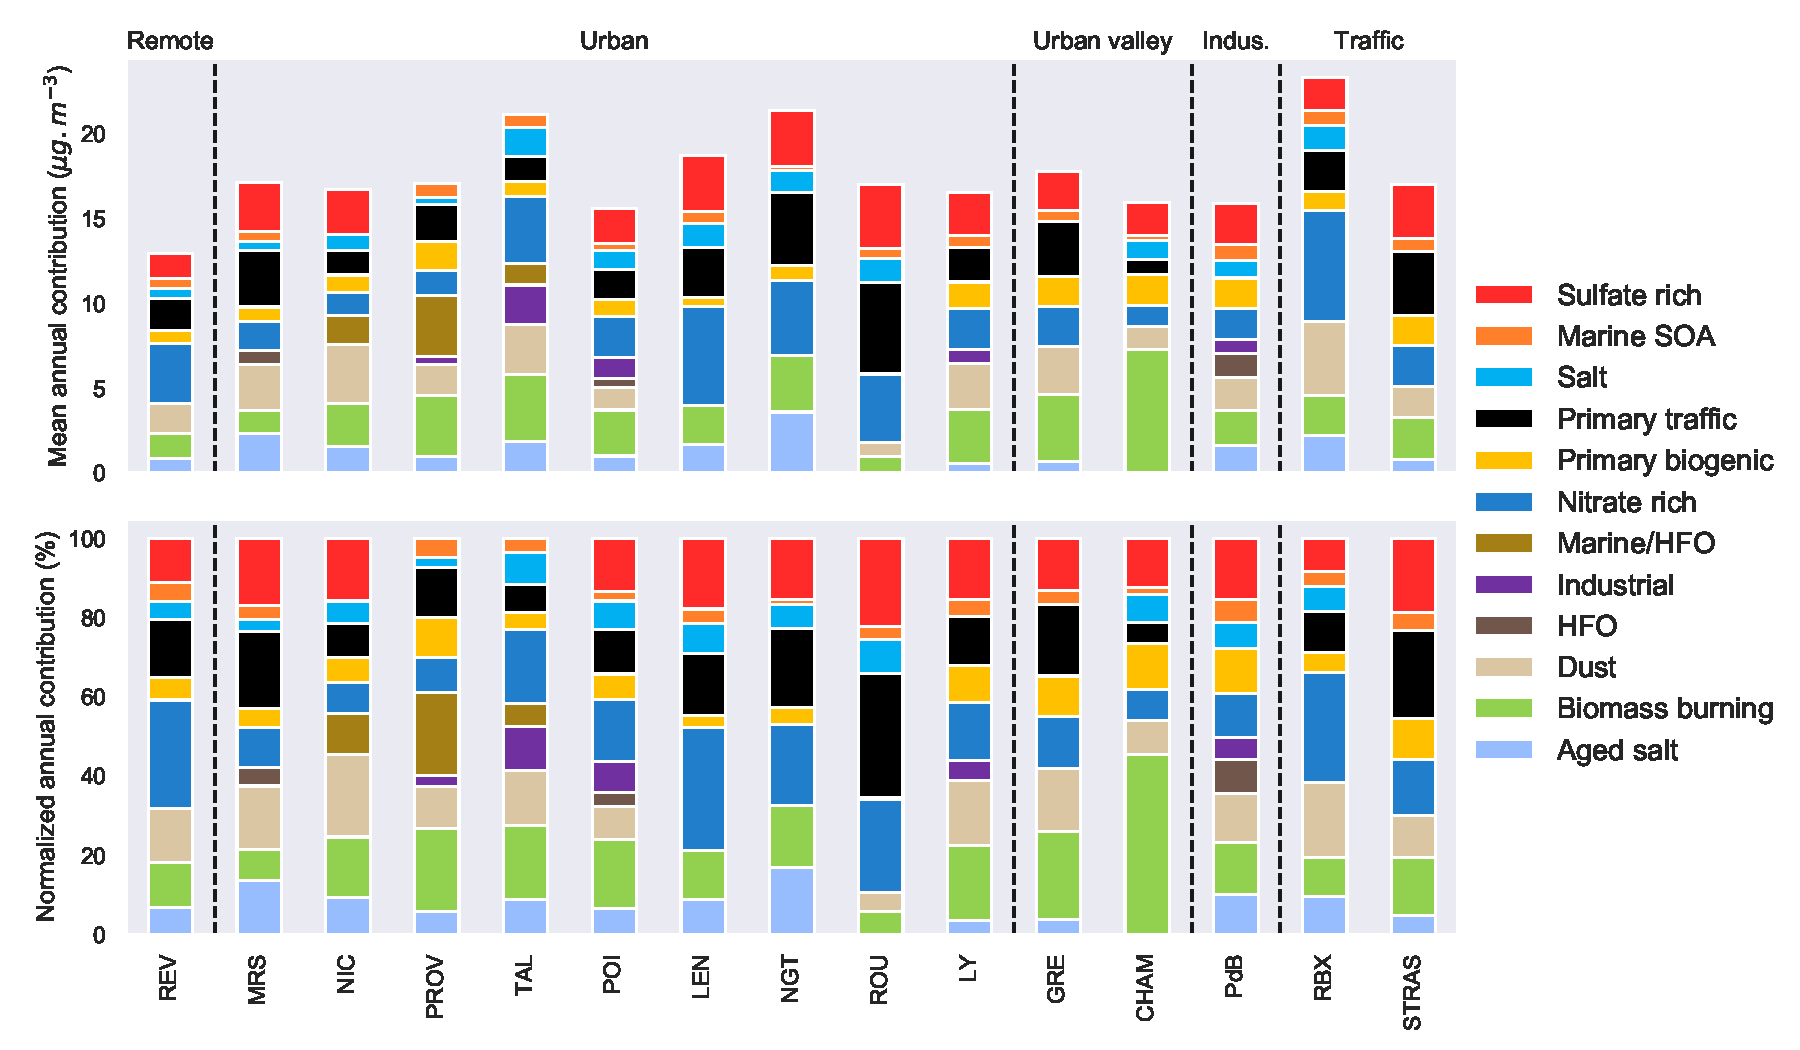
\includegraphics[width=1\linewidth]{chapter03/fig2.pdf}
    \caption{Yearly average contributions from the constrained runs in
        \si{\concum} (\textbf{top}) and \si{\percent} (\textbf{bottom}) of the identified factors to
        \PM{} mass at each of the sites studied, grouped by typology (remote, urban,
urban valley and traffic).} 
\label{fig:fig2}
\end{figure}

\begin{figure}[ht]
    \centering
    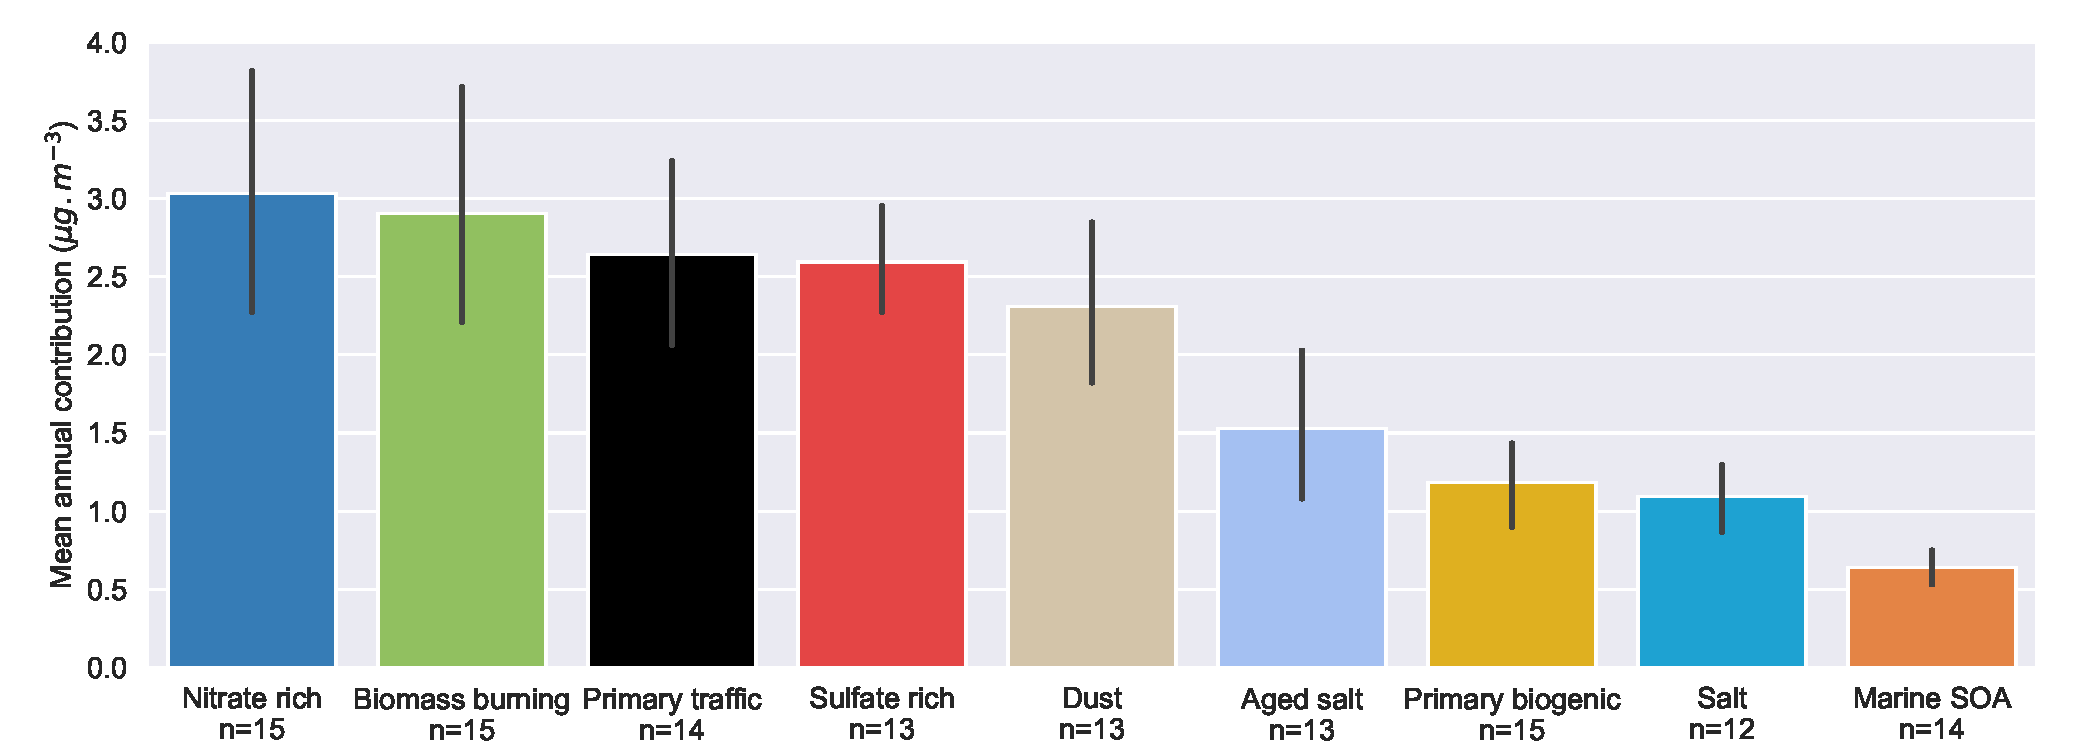
\includegraphics[width=1\linewidth]{chapter03/fig3.pdf}
    \caption{Average daily mass concentrations (\si{\concum}) of the main PMF factors
        (observed at least at 10~sites) obtained in the constrained runs in
        this study. Error bars indicate the standard deviation between sites
        and $n$ denotes the number of sites where the factors were identified.}
    \label{fig:fig3}
\end{figure}


\subsection{Seasonality of the~Contributions}%
\label{sub:seasonality_of_the_contributions}

Since it is not possible to present all the results in this paper, we encourage the reader
to refer to the online view app to browse the different time series and chemical profiles.
Among~the factors that present a strong seasonality (nitrate rich, biomass burning,
primary biogenic and marine SOA) we choose to highlight the seasonal contributions of the
biomass burning (main contribution during winter) and the primary biogenic (main
contribution during summer) (Figures~\ref{fig:fig4} and~\ref{fig:fig5}, respectively).

With about {35}{\%} of the \PM{} mass during winter and less than {2}{\%} during summer
(see Figure~\ref{fig:fig4}), the~biomass burning factor shows the strongest seasonality
among all factors identified. At~the two sites investigated in the Alpine valley, and~due
to frequent inversion layers in winter, the~contribution of the biomass burning can reach
up to {70}{\%} of the total \PM{} mass in the cold season, as~already mentioned in
previous studies in the
Alps~\autocite{favezIntercomparison2010,bonvalotEstimating2016,srivastavaSpeciation2018,herichOverview2014}.

Conversely, the~primary biogenic factor can contribute to a significant amount of \PM{}
during the warm months, with~an average contribution to \PM{} of \SI{13\pm8}{\percent}
(min \SI{1.5}{\percent}, max \SI{33}{\percent} among the sites studied) during summertime,
as~shown in Figure~\ref{fig:fig5}. A~detailed study about the seasonal and spatial
variations of the primary biogenic factor resulting from these PMF analyses can be found
in~\mbox{\textcite{samakePolyols2019}}.

\begin{figure}[ht]
    \centering
    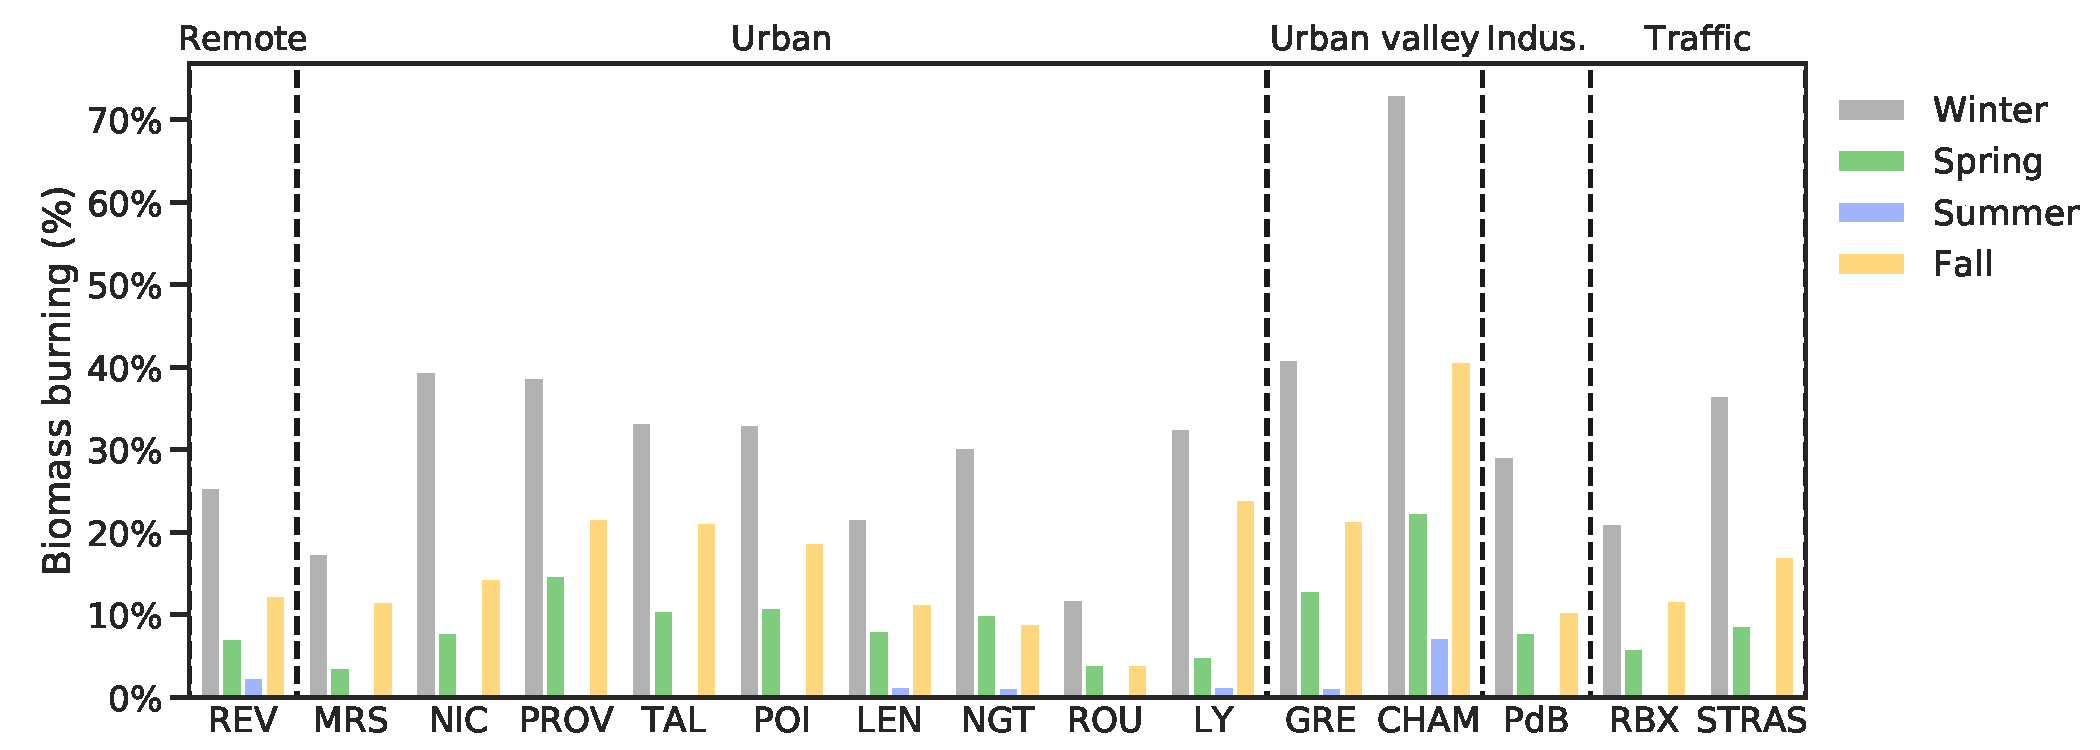
\includegraphics[width=1\linewidth]{chapter03/fig4.pdf}
    \caption{Biomass burning seasonal contributions (in \si{\percent}) to the total PM mass
    from the constrained~runs.}
    \label{fig:fig4}
\end{figure}

\begin{figure}[ht]
    \centering
    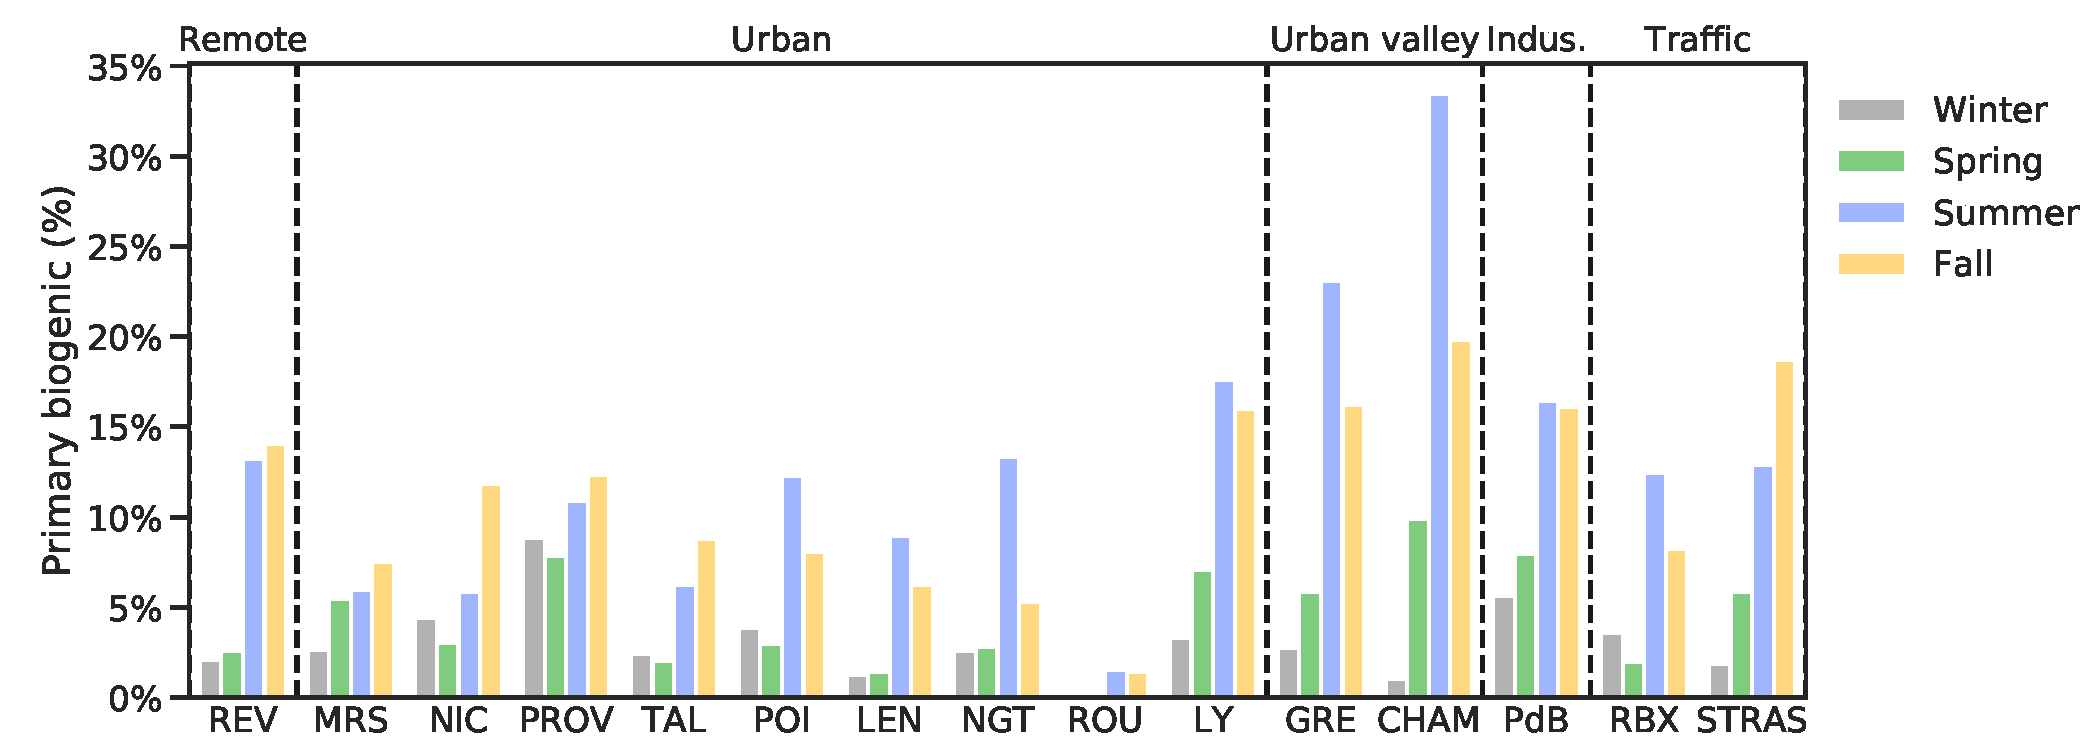
\includegraphics[width=1\linewidth]{chapter03/fig5.pdf}
    \caption{Primary biogenic seasonal contributions (in \si{\percent}) to the total PM mass
    from the constrained runs.}
    \label{fig:fig5}
\end{figure}


\subsection{Uncertainties of PMF Factors}%
\label{sub:uncertainties_of_pmf_factors}

In factor analysis, three sources of uncertainties can arise from: (1) random errors in
data values linked to measurement uncertainties: (2) rotational ambiguity due to possible
multiple acceptable solutions; and  (3) modeling errors, such as mis-specification of the
model compare to the real processes in atmosphere~\autocite{belisEuropean2014}.

To quantify the uncertainties of the results at one site (internal uncertainties), and~the
variability of the factor profiles, we performed both bootstrap (BS) and displacement
(DISP) analyses. Shortly, BS randomly resample the $X$ matrix and perform a new PMF run,
then try to map each new BS-factor to the reference run, according to the correlation
between the contributions of factors. A~threshold correlation coefficient of 0.6 was used
for all sites in this study. BS gives an estimation of uncertainties linked to sampling
artifact and measurement uncertainties. DISP analysis estimates the rotational ambiguity
by lowering and majoring each species in every factor up to a given variation of the $Q$
value dQmax. The~reader may refer to~\textcite{paateroMethods2014} for more details about
DISP computation in EPA PMF5.0. Here, BS and DISP analyses were applied in both base runs
and constrained runs, i.e.,~before and after applying the constraints listed in
Table~\ref{tab:constraints}.


\subsubsection{Statistical Stability of the~Solutions}%
\label{ssub:statistical_stability_of_the_solutions}

In this study, all base cases solutions (i.e., without constraints) reached high BS
values, the~lowest one being {77}{\%} (Table~\ref{tab:BSmapping}).  Hence, the~PMF base
solution for all sites already presents very good BS mapping results that largely agree
with the general recommendations of the European guide on air pollution source
apportionment with receptor models~\autocite{belisEuropean2014}. Moreover, we
systematically observed improvement in BS mapping when applying constraints
(Table~\ref{tab:BSmapping}).  Considering all the sites, the~minimum value of BS for
constraint solutions was \SI{83}{\percent}. It means that, even if the base cases were
good enough to differentiate specific factors, the~expert knowledge added through the use
of specific constraints helped the model to ``clean'' the factors and improve the
stability of the solutions. Finally, we note that virtually no ``unmapped'' factor was
obtained during this BS sensitivity analysis (always less than {1}{\%}).  Concerning the
DISP analyses, no swap between factors was observed,   for both the base and
constrained~runs.

\begin{table}[ht]
    \centering
    \caption{
        Summary of bootstrap mapping of the base runs and of the constrained
        runs expressed as percent of correct mapping bootstrap for the main
        factors identified in this study. Ranges are min and max. The~number in
        parenthesis is the number of sites where the given profile could be
        identified.
    }
    \label{tab:BSmapping}
	\footnotesize
    \begin{tabular}{lScSScS}
        \toprule
                        & \multicolumn{3}{c}{\textbf{Base Cases}} & \multicolumn{3}{c}{\textbf{Constrained Cases}}\\
\textbf{Profiles}                & {\textbf{Mean $\pm$ Std}} & \textbf{Range} & {\textbf{Unmapped}} & {\textbf{Mean $\pm$ Std}} & \textbf{Range} & {\textbf{Unmapped}}\\
        \midrule
Biomass burning (15)    & 100.0\pm0.0    & 100--100 & 0.0        & 100.0\pm0.0    & 100--100 & 0.0\\
Nitrate rich (15)       & 98.7\pm2.8     & 89--100  & 0.2        & 99.9\pm0.3     & 99--100  & 0.0\\
Primary biogenic (15)   & 99.3\pm1.3     & 96--100  & 0.0        & 99.8\pm0.8     & 97--100  & 0.0\\
Marine SOA (14)         & 95.9\pm4.9     & 83--100  & 0.7        & 100.0\pm0.0    & 100--100 & 0.0\\
Primary traffic (14)    & 97.1\pm4.8     & 85--100  & 0.0        & 98.7\pm2.8     & 89--100  & 0.0\\
Aged sea-salt (13)      & 95.8\pm4.8     & 83--100  & 0.1        & 98.5\pm2.7     & 91--100  & 0.1\\
Sulfate rich (13)       & 93.4\pm6.9     & 83--100  & 0.5        & 98.9\pm1.8     & 95--100  & 0.1\\
Dust (12)               & 94.1\pm7.3     & 77--100  & 0.7        & 97.8\pm4.8     & 83--100  & 0.1\\
Sea-salt (11)           & 99.5\pm1.5     & 95--100  & 0.0        & 99.8\pm0.6     & 98--100  & 0.0\\
Industries (5)          & 92.8\pm8.5     & 80--100  & 1.0        & 98.4\pm2.2     & 96--100  & 0.0\\
        \bottomrule
    \end{tabular}
\end{table}

\subsubsection{Uncertainties of the Profile~Composition}%
\label{ssub:uncertainties_of_the_profile_composition}

\paragraph{Impacts of the Constraints on the Uncertainties}%
\label{par:impacts_of_the_constraints_on_the_uncertainties}

The application of specific chemical constraints (see Table~\ref{tab:BSmapping}) also
improved the resolving power of the PMF and the quality of the solutions, displaying
narrower uncertainties for the contributions of chemical species in many factors.
For~instance, the~OC* concentration in the primary traffic profile of ROU   varied between
0.79 and \SI{1.65}{\concum} for the base run but only between 1.23 and \SI{1.84}{\concum}
in the constrained run, according to the BS analysis (5{th}--95{th})
(Table~\ref{tab:uncertainties_constraints}). Similar trends were observed for the
uncertainties proposed by the DISP approach and were apparent for most of the chemical
species that are proxies of a given source (Table~\ref{tab:uncertainties_constraints}
proposes some examples).

Interestingly, the~uncertainties estimated with the DISP method were almost always
narrower than the uncertainties given by the BS method. This may be explained by using
constraints that already narrowed the rotational ambiguity (lowering DISP uncertainties
range) or by the sensitivity of our datasets to specific days (increasing BS uncertainties
range).

\paragraph{Composition Uncertainties in the Chemical Profiles}%
\label{par:composition_uncertainties_in_the_chemical_profiles}

The dispersion of the concentrations of key species in different profiles was investigated
and is briefly presented here. The~external variability (from site to site) is presented
in its own section below
(Section~\ref{sub:variability_of_the_chemical_profiles_at_the_regional_scale}).  Here, we
only assessed the internal variability, i.e.,~the variability of a specie at a given site
for a given factor, and~the coefficients of variation (CV, standard deviation over the
mean) of species from the BS runs are presented in Figure~\ref{fig:fig6}, averaged from
all sites.      To minimize the impact of potential outliers in the BS runs, only the BS
values above the 5{th} percentile and below the 95{th} percentile were~used.

\begin{sidewaystable}
    \centering
    \caption{Summary of the uncertainties (in \si{\concum}) obtained from the BS
        (5{th} and 95{th} percentiles) and DISP
        (min-max) runs for a subset of species in two different factor profiles,
        the road traffic at ROU site and the biomass burning at GRE site, for both
      the base and constrained runs}
    \label{tab:uncertainties_constraints}
    \begin{tabular}{lcccccccc}
        \toprule
        & \multicolumn{8}{c}{\textbf{ROU---Primary Traffic}}\\
       \textbf{ Run} & \multicolumn{4}{c}{\textbf{Base}} & \multicolumn{4}{c}{\textbf{Constrained}} \\
        \midrule
\textbf{Species} & OC* & EC & Cu & Fe & OC* & EC & Cu & Fe\\
Reference  & 1.605 & 0.541 & 0.0104 & 0.1986 & 1.649 & 0.592 & 0.0114 & 0.221\\
BS (5{th}--95{th}) & 0.792--1.654 & 0.334--0.541 & 0.007--0.011 & 0.108--0.232 & 1.232--1.845 & 0.493--0.641 & 0.009--0.013 & 0.159--0.264\\
DISP (min-max) & 1.426--1.912 & 0.480--0.644 & 0.009--0.012 & 0.178--0.229 & 1.576--1.837 & 0.572--0.666 & 0.011--0.012 & 0.210--0.236 \\
        \toprule
        & \multicolumn{8}{c}{\textbf{GRE---Biomass Burning}}\\
\textbf{Run} & \multicolumn{4}{c}{\textbf{Base}} & \multicolumn{4}{c}{\textbf{Constrained}} \\
        \midrule
Species & OC* & EC & Levoglucosan & K+ & OC* & EC & Levoglucosan & K+\\
Reference & 1.266 & 0.434 & 0.306 & 0.057 & 1.520 & 0.563 & 0.388 & 0.059\\
BS (5{th}--95{th}) & 1.061--1.505 & 0.372--0.614 & 0.269--0.362 & 0.039--0.067 & 1.347--1.640 & 0.492--0.672 & 0.412--0.434 & 0.039--0.070\\
DISP (min-max) & 1.100--1.363 & 0.378--0.480 & 0.275--0.319 & 0.050--0.061 & 1.456--1.589 & 0.539--0.604 & 0.408--0.439 & 0.058--0.059\\
\bottomrule
    \end{tabular}
\end{sidewaystable}



For most of the main proxies of sources (i.e., specific tracers), we observed a narrow
range of possible values given by the BS and DISP, associated with low CV for the specific
tracers. This is the case for instance for the levoglucosan in the biomass burning factor
(\SI{1.6\pm0.5}{\percent}), the~MSA in the marine SOA (\SI{1.2\pm0.8}{\percent}),
the~polyols in the primary biogenic (\SI{0.1\pm0.1}{\percent}), the~Ti in the dust
(\SI{12.2\pm9.6}{\percent}), the~\ce{Na+} in the sea-salt (\SI{10.3\pm7.2}{\percent}),
NO3- in the nitrate rich (\SI{6.5\pm2.5}{\percent}) or even Cu and Sb in the primary
traffic (\SI{14.0\pm11.0}{\percent} and \SI{16.0\pm12.4}{\percent}, respectively, which
are the lowest CVs for these two metals for all factors).

However, for~non-tracers species, the~dispersion according to the BS and DISP runs could
be larger. For~instance, according to BS, the~OC* and \ce{Ca^2+} in the nitrate rich have
a CV of \SI{60.4\pm35.9}{\percent} and \SI{59.6\pm39.1}{\percent}, respectively, or~the
metals in the primary biogenic factor.

We also note that some species have an extremely large CV in some factors, notably the
\ce{NO3^-} in the sulfate rich factor (\SI{354.3\pm301.3}{\percent}). This likely
indicates some possible mixing with other factor or more generally the fact that the PMF
model did not find a well defined solution for this species in this factor. Conversely, we
can see in Figure~\ref{fig:fig6} that the main species with regard to the mass are stable
in the biomass burning factor. Notably,  ~\PM{}, OC* and EC had CVs of
\SI{12.2\pm6.8}{\percent}, \SI{12.8\pm8.9}{\percent} and \SI{25.6\pm22.9}{\percent},
respectively, an~indication that the components of this factor  were well described by the
PMF~run.

Therefore, despite high confidence in the markers and in the obtained mass fractions,
caution should be taken when scrutinizing the repartition of a given species between
factors and extrapolating specific ratio if the species present some large~uncertainties.

\begin{figure}[ht]
    \centering
    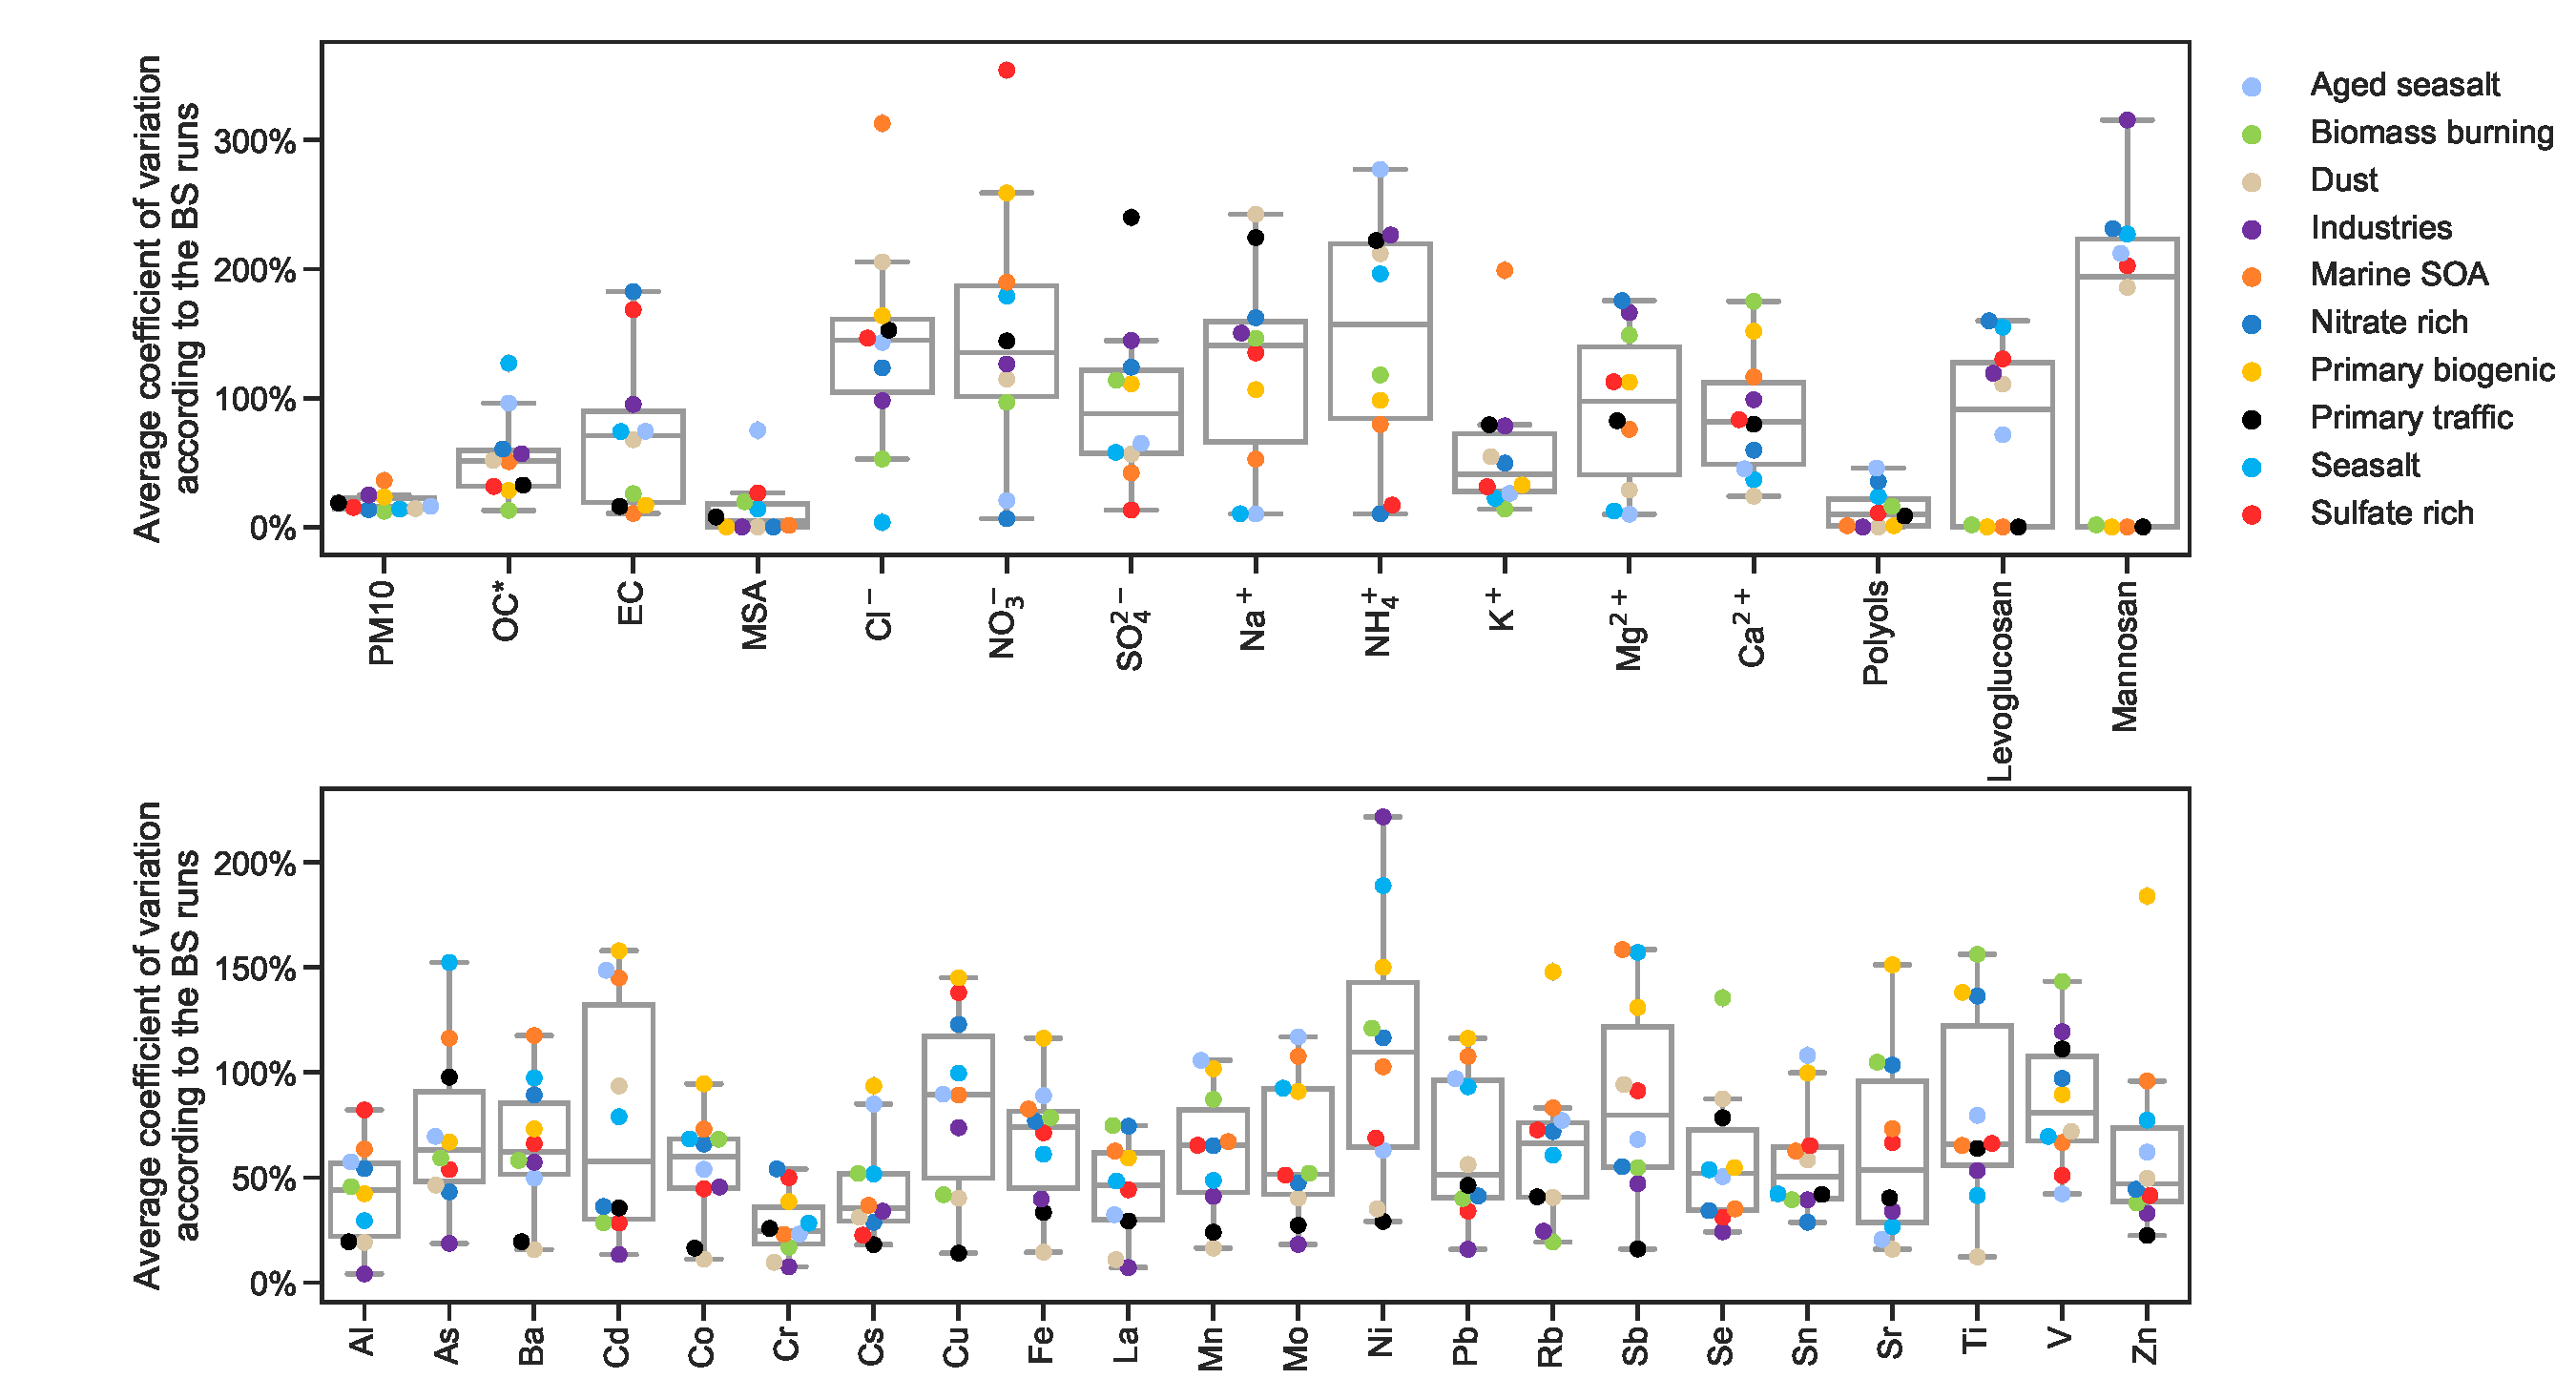
\includegraphics[width=.85\linewidth]{chapter03/fig6.pdf}
    \caption{
        Site averaged coefficient of variation of the species concentration in
        each major profile according to the BS runs. Markers are individual
        values and the box plots show  the dispersion of values.
    }
    \label{fig:fig6}
\end{figure}

\subsection{Estimation of the Uncertainties of Time Series~Concentrations}%
\label{sub:estimation_of_the_uncertainties_of_time_series_concentrations}

This section presents an attempt to express the uncertainties associated with the
concentrations of a chemical species in the time series of a specific factor contribution.
Even if during the BS runs both the $F$ and $G$ matrices  were recomputed, only the $F$
matrix was returned to the user in the EPA PMF5.0 software. The~matrix $G$ was only used
internally to map the BS factor to the base factor~\autocite{paateroMethods2014}. As~a
result, the~outcome  was an estimation of uncertainties for the $F$ matrix, but~not for
the $G$ one.  Hereafter, we propose to estimate the uncertainties for the time series of
the concentrations of a chemical species by multiplying the different concentrations given
by the uncertainties runs (BS and DISP) by the factor contribution of the reference run
$G_{ref}$:

\begin{equation}
    X'_{ERRi} = F_{ERRi} \cdot G_{ref},
\end{equation}

where $F_{ERRi}$ refers either to the $F$ matrix given by the DISP min/max run or to one
of the BS runs, $G_{ref}$ is the contribution matrix of the reference run, and~$X'_{ERRi}$
simulates the temporal concentration of species in the run $ERRi$ (DISP or BS). It should
be noted that this method only represents an approximation of the ``true'' uncertainties
of the model over the sample time series. Indeed, both the $F$ and $G$ matrix should
theoretically be modified at the same time, whereas the different $F_{ERRi}$ were
multiplied here by a constant value of $G$ for a given sample.  Therefore, samples with
high concentration ($G$) will always have higher uncertainties than sample with
low~concentration.

However, this method provides a first idea of the uncertainties in the time series and
help to visualize the uncertainties given by the BS and DISP methods.  For instance,
uncertainties (i.e., standard deviation of BS, and~DISP min/max) of the OC* in the
sulfate-rich factor obtained for the site CHAM are presented in Figure~\ref{fig:fig7},
coupling the uncertainties in the chemical profile (OC*\textsubscript{ref},
\SI{0.5423}{\concum}; OC*\textsubscript{BS}, \SI{0.568\pm0.262}{\concum}; and
OC*\textsubscript{DISP}, \SIrange{0.612}{0.934}{\concum}) and the concentrations time
series. In~this example, it may be hypothesized that the sulfate-rich factor may be mixed
with another aerosol fraction (e.g., possibly SOA) since it presents some important
uncertainties and high concentration of OC* during summertime.  Even if it may be possible
by directly tweaking the ME-2, the~solver used in EPA PMF5.0 software, it seems difficult
for the non-computers-scientist end-user to extract the different $G$ matrices. We think
that an added value to the software would be to output them during the BS process and we
encourage developers of other PMF software to ease this~process.

\begin{figure}[ht]
    \centering
    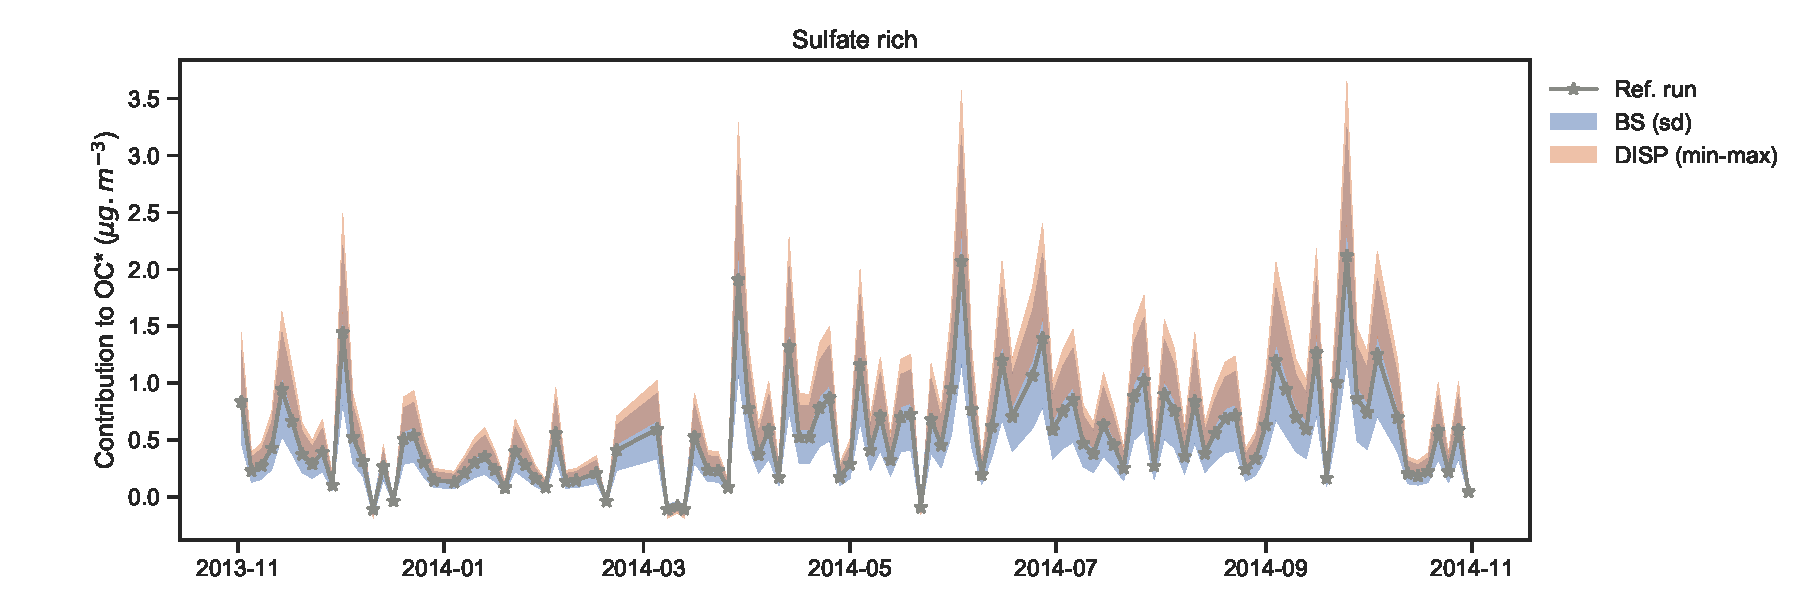
\includegraphics[width=1\linewidth]{chapter03/fig7.pdf}
    \caption{
        Estimation of the over-time uncertainties of OC* (in \si{\concum}) in the
        sulfate-rich factor at CHAM site using the BS and DISP runs. The grey line denotes
        the reference constrained run contribution, the~shaded blue area indicates the
        uncertainties (standard deviation) given by the BS and the orange shaded area the
        uncertainties given by the DISP (min max).
    }
    \label{fig:fig7}
\end{figure}

\subsection{Variability of the Chemical Profiles at the Regional~Scale}%
\label{sub:variability_of_the_chemical_profiles_at_the_regional_scale}

\subsubsection{Overall~Comparison}%
\label{ssub:overall_comparison}

In the previous sections, we discuss  the internal variability of the different factors.
Next,~similarities of all the chemical profiles identified in this study were investigated
thanks to the tools developed in the frame of the FAIRMODE (Forum for Air Quality
Modeling) activities and presented by~\textcite{belisNew2015}, based on the constrained
runs. PMF factor profiles attributed to a source category are compared among each other's
using both the PD (Pearson distance) and SID (standardized identity distance) similarity
indicators. Fewer factors identified at some sites were not considered in this assessment
analysis as they showed some mixing with other emission~sources.

Figure~\ref{fig:fig8} gives mean and standard deviation of the distances between all pair
of factor/source profiles tagged as belonging to the same category in the SID-PD space. It
results in the comparison of $n\times\frac{n+1}{2}-n$ pairs of profiles for each category,
where n is the number of profiles belonging to the same source category (see
Figure~\ref{fig:fig8}).

\begin{figure}[ht]
    \centering
    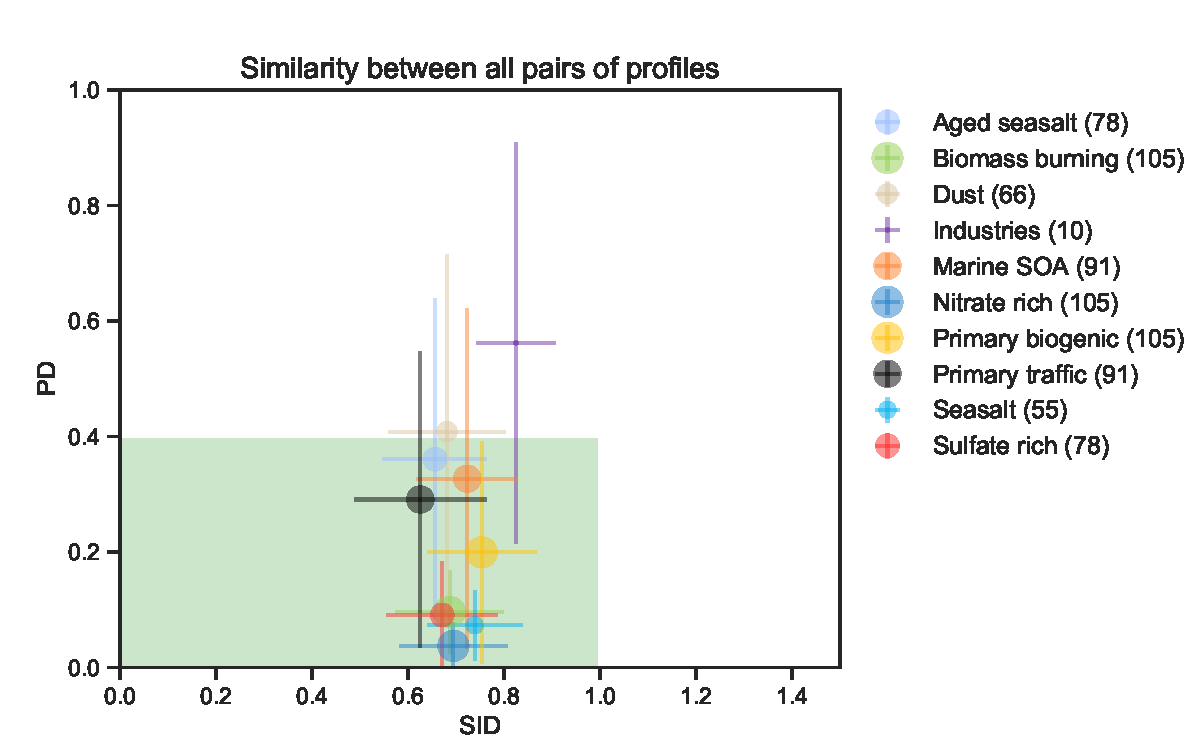
\includegraphics[width=0.8\linewidth]{chapter03/fig8.pdf}
    \caption{
       Similarity plot for all pairs of profiles belonging to the same
        factor/source category in this study. The~mean $\pm$ standard deviation
        for a given source category are plotted. The~size of the dot is
        proportional to the number of available pair of profile (from 10 to 105,
        shown in parenthesis in the legend). The~green box highlights the
        acceptable area for profile similarity according
        to~\textcite{pernigottiDeltaSA2018}.
    }
    \label{fig:fig8}
\end{figure}

First, we can see that many factor/source profiles present low PD and SID with values
(mean $\pm$ standard deviation) inside the acceptance box ($PD<0.2$ and $SID<0.8$),
indicating that they are stable over the different sites of the study.  It includes the
biomass burning, sulfate-rich, nitrate-rich, and~fresh sea-salt factors. The~primary
biogenic source also appears relatively stable at all sites but presents some
dissimilarity according to the PD metric. It suggests that this source is not yet fully
understood and need further investigation, as~recently discussed
by~\textcite{samakePolyols2019}.

Other factors seem to have more heterogeneous profiles, with~part of their values (mean
$\pm$ standard deviation) outside of the acceptance box. For~instance, differences  were
clearly observed in the few industrial chemical profiles. This is expected as such
emissions may be very local and highly variable, despite their common contents of high
concentrations of metals and metalloids. Marine SOA profiles also display site-to-site
variations and a wide range in the PD-SID space, notably for the PD metric. This factor,
mainly identified thanks to its MSA marker, may actually regroup a large diversity of
chemical species. The~low variance in the SID but high variance in the PD tends to
indicate a large discrepancy for the chemical species that represent the main mass of the
profile. A~deeper analysis (not presented here) showed  that the high variance is driven
by an observation at only three sites: GRE, CHAM and ROU. The~valley sites of GRE and CHAM
both present a larger part of OC* in their profile while, conversely, ROU presents the
lowest amount of OC* among all the sites.  Finally, the~primary traffic profile presents
the lowest SID values, but~a relatively high PD, still in the acceptable area. As~this
factor is commonly observed in RM studies and contributes substantially to the \PM{} mass,
it is discussed in detail in the following~section.

\subsubsection{A Non-Homogeneous Source: Primary~Traffic}%
\label{ssub:a_non_homogeneous_source_primary_traffic}

The primary traffic source present large variability in the SID-PD space, suggesting a
wide variety of road transport chemical profiles over France. As~a matter of fact, this
factor presents the lowest SID value of all profile while larger variabilities  were found
in the PD metric. This could be seen in the OC/EC ratio, both species being the most
abundant ones within the primary traffic factor
(Figures~\ref{fig:fig9}~and~\ref{fig:fig10}). Even  when excluding the rural site of REV,
we observed a large variability in this ratio, spanning from 0.09 to 3.31
(Figure~\ref{fig:fig10}). As~the PD is mainly sensitive to the main chemical species in
term of mass, these two compounds may explain the wide span of the PD value for this
source.  It should also be noted that the high variability in the PD may be driven by the
values for the RBX site. Indeed, despite RBX has all   22 metals in the ranges of the
other sites, the~value of OC* is extremely low compared  to others sites. The~lower
dispersion in the SID-axis highlights the relative homogeneity of the other components of
this factor. Indeed, as~shown in Figure~\ref{fig:fig9}, the~amount of metals, notably the
Fe, Cu, Al, Zn and Sb, as~well as  sulfate are relatively homogeneous over the 14 sites.
We also see that organic compounds such as levoglucosan, mannosan, MSA and polyols as well
as \ce{Na+} are almost never present in this factor, or~in a very small~amount.

The extremely high OC-to-EC ratio for REV (Figure~\ref{fig:fig10}) and the relatively
higher uncertainties estimated from the BS runs (OC*\textsubscript{BS},
\SIrange{0.000}{0.937}{\concum}; EC\textsubscript{BS}, and
\SIrange{0.0162}{0.0703}{\concum}, still close to the detection limit) indicate  low
confidence in the PMF solution for this factor at this~site.

Finally, the~primary traffic factor is the closest to the dust factor when comparing the
dust factor to all other profiles (see   Figure S1). Such results may indicate that some
resuspended dust coming from road abrasion or resuspension might contribute importantly to
the dust factors at some sites.  This may also explain the relatively low amount of trace
element in the primary traffic factor obtained at STRAS. Indeed, at~this site, we
identified a mixed factor of ``resuspended dust'',  which  may be a mixing between mineral
dust and road dust. This particular factor is not included in the ``dust'' one presented
in Figure~\ref{fig:fig8} due to it~singularity.

\begin{figure}[h]
    \centering
    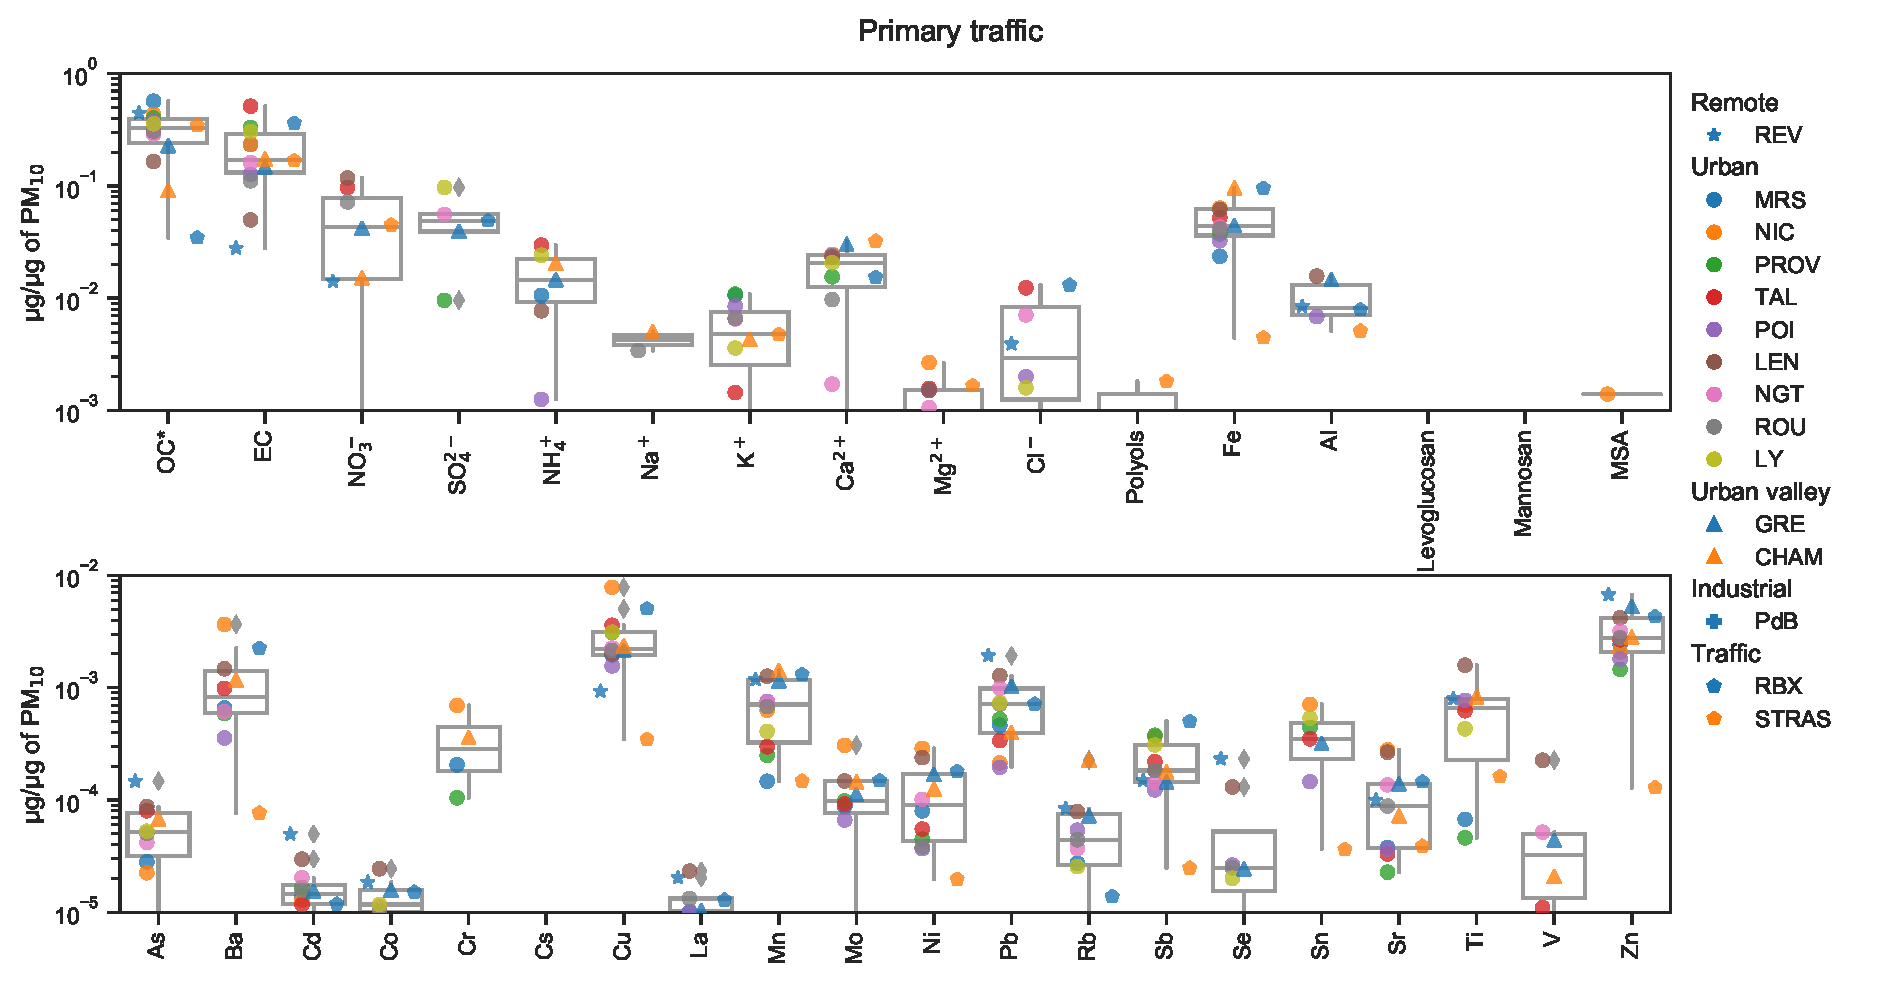
\includegraphics[width=1\linewidth]{chapter03/fig9.pdf}
    \caption{
        Chemical profiles obtained for the primary traffic factor in
        \si{\micro\gram} per \si{\micro\gram} of \PM{}. Markers refer to
        individual site and box plots show the dispersion for all sites.
    }
    \label{fig:fig9}
\end{figure}


\begin{figure}[h]
    \centering
    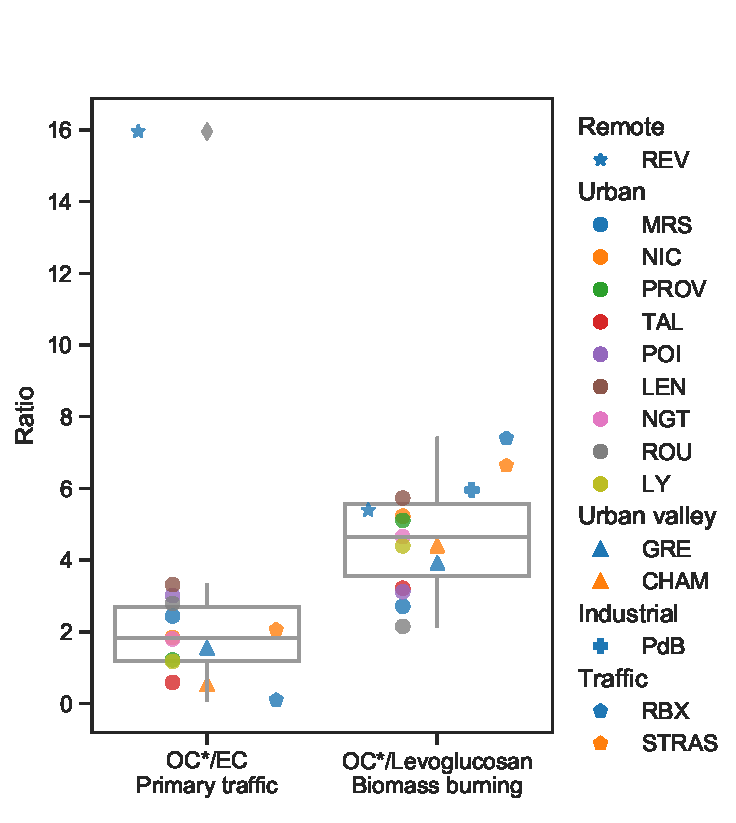
\includegraphics[width=0.5\linewidth]{chapter03/fig10.pdf}
    \caption{
        Variability of the OC-to-EC ratios and OC-to-Levoglucosan ratios obtained
        for the primary traffic and biomass burning factors, respectively.
        Markers refer to individual site and box plots show the dispersion for
        all sites.
    }
    \label{fig:fig10}
\end{figure}

\subsubsection{A Homogeneous Source: The Biomass Burning~Source}%
\label{ssub:a_homogeneous_source_the_biomass_burning_source}

Among the stable profiles, the~biomass burning is the most important source in terms of
mass contribution. As~already well reported in the
literature~\autocite{schauerMeasurement2001, schmidlChemical2008, belisCritical2013},  ~OC
is the PM dominant fraction in this source, with~a quite constant amount
(\SI{38\pm5}{\percent} of the PM mass, see Figure~\ref{fig:fig11}). Moreover, as~presented
in Figure~\ref{fig:fig6} and detailed in Figure S2, the~OC* uncertainties in this factor
is low. Concerning the tracer of biomass burning,   levoglucosan and mannosan  are present
at \SI{96\pm3}{\percent} and \SI{95\pm4}{\percent} in this profile, respectively
(Figure~\ref{fig:fig11}). Mass-wise, the~levoglucosan represents \SI{8\pm2}{\percent} of
the total PM mass. The~EC presents a wider dispersion, with~a mass concentration of
\SI{9\pm4}{\percent}. We also note a fair amount of \ce{Cl-}, as~well as \ce{K+} in this
factor, which explains \SI{14\pm19}{\percent} and \SI{32\pm13}{\percent} of their
respective total mass. Despite its contribution to the mass of biomass burning PM mass
(\SI{6\pm4}{\percent}), the~\ce{NO3^-} is clearly not mainly allocated to this source as
the biomass burning represents only \SI{7\pm5}{\percent} of the total \ce{NO3^-} mass.
Metal elements are barely present in this factor and some high discrepancy  was observed
for the different sites, with~a dispersion up to two orders of magnitude for Pb, Zn and
Mn.  It may be noted that the OC-to-Levoglucosan ratio fluctuates between 2.1 and 7.4,
with~a mean and standard deviation values of \num{4.6\pm1.5} (Figure~\ref{fig:fig10}).
Such ratios are in the 1.9--12.6 range of values previously reported for \PM{} wood
combustion samples~\autocite{schauerMeasurement2001, schmidlChemical2008}. They may
reflect the use of the different type of wood for heating purposes, as~detailed in the
same previous studies. However, we did not observe any systematic difference according to
the geographical location and/or the site typology for this source.  Overall, these
findings suggest a relatively similar wood burning emission in term of PM constituents all
over the~territory.

\begin{figure}[ht]
    \centering
    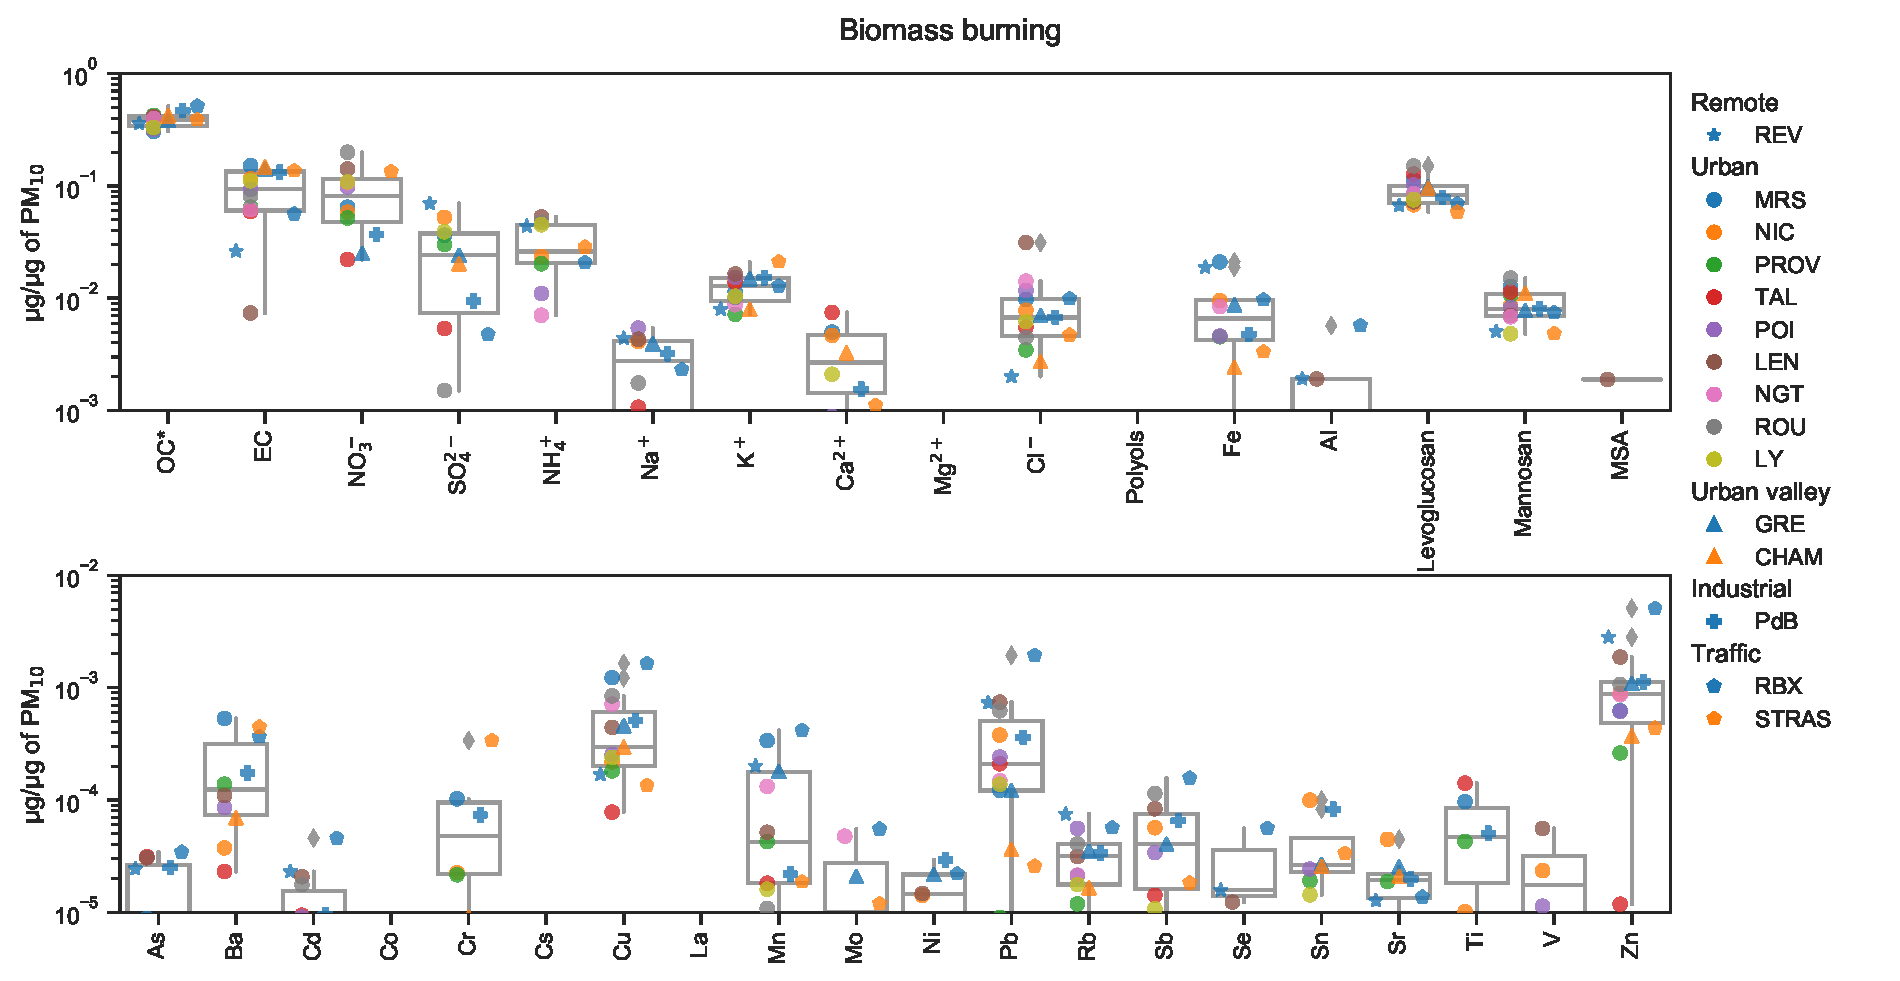
\includegraphics[width=1\linewidth]{chapter03/fig11.pdf}
    \caption{
        Chemical profiles obtained for the biomass burning factor in
        \si{\micro\gram} per \si{\micro\gram} of \PM. Markers refer to
        individual site and box plots show the dispersion for all sites.
    }
    \label{fig:fig11}
\end{figure}
%\clearpage
\section{Conclusions}%
\label{sec:conclusion}

This paper presents results obtained from PMF analyses conducted in a harmonized way and
taking advantage of datasets corresponding to more than \num{2200} samples collected at 15
different sampling sites in France. To~the best of our knowledge, this is the first study
using such a large database over several years of monitoring. Thirty-seven input variables
were selected to cover a wide range of major expected \PM{} factors and to optimize total
mass reconstruction at all sites.  The operator-related subjectivity was reduced by using
homogeneous statistical and geochemical criteria for the source discrimination
and~identification. 

Overall, the main \PM{} factors were found to be primary traffic (\SI{15\pm7}{\percent} of
the \PM{} mass on a yearly average) and biomass burning (\SI{17\pm9}{\percent}) as well as
two secondary aerosol fractions dominated by ammonium nitrate (\SI{17\pm8}{\percent}) and
ammonium sulfate (\SI{15\pm4}{\percent}), respectively. These findings are in good
agreement with what has   commonly been observed by many previous studies over Europe and
illustrates ---if still needed---the major impact of anthropogenic emissions on urban air
quality. Nevertheless, substantial contributions of mineral dusts (\SI{13\pm4}{\percent}),
fresh (\SI{6\pm2}{\percent}) and/or aged sea-salts (\SI{8\pm4}{\percent}), as~well as of
primary biogenic aerosols (\SI{7\pm3}{\percent}) are also observed at almost all sites,
reflecting that natural emissions should not be neglected as other important contributors
to \PM{} levels on a yearly~basis.

During wintertime, high contribution of the biomass burning  was observed, together with
the nitrate-rich factor in early spring (March). The~sea-salt also presents higher
contribution during this period of the year, potentially linked to stronger westerlies
winds.  In summer, all sites present important contributions from biogenic sources: the
primary biogenic and marine SOA factors.  Conversely, the~primary traffic, dust, aged
sea-salt and sulfate rich factors do not present clear seasonality~pattern.  Uncertainties
of each PMF results were investigated thanks to the bootstrap and displacement methods,
both for the base and the constrained runs. The~use of a set of constraints---taken as
limited as possible---allows to decrease these uncertainties and to strengthen the output
statistical representativity of factors commonly observed all over the French continental
territory.  The internal variability (i.e., for a given site) assessment shows high
confidence for the concentration of the main proxies of sources (i.e., specific tracers)
and for the \PM{} mass apportionment, but~larger uncertainties were  found for
concentrations of non-tracer species and caution should be taken concerning the
contributions of such chemical species to the different~factors.

Finally, the~external variability (i.e., from one site to another) was investigated thanks
to both the SID and PD metrics.  In~particular, the~discrepancy between the chemical
profiles of sources could be quantified thanks to both the SID and PD metrics, notably
showing that fresh sea salt, nitrate-rich, sulfate-rich and biomass burning factor
profiles can be considered as chemically similar at all the sites studied. Conversely,
some significant variabilities were observed for other factor chemical profiles, such as
the ones related to traffic and industrial emissions as well as mineral dusts and marine
SOA. The~latter finding is calling for the use of additional variables, such as organic
molecular markers, within~studies aiming at scrutinizing specific local sources at
individual sites and/or for a better knowledge on the origins of SOA~fractions.

Overall, results obtained in this comprehensive study may help to increase the
completeness of the SPECIEUROPE database, and~can be used to assess the contributions of
the different sources to the oxidative potential of \PM{} following methodology proposed
by~\textcite{weberApportionment2018}.



%% Acknoledgment
% This work has been conducted as part of the SOURCES project funded by ADEME
% (grant agreement no. 1462C0044). The PhD of Samuël Weber is founded by ENS
% Paris. Samples were notably collected and analyzed in the frame of various
% programs funded by the French Ministry of Environment through the CARA program
% leaded by the National Reference Laboratory for Air Quality Monitoring (LCSQA)
% and/or through programs (such as Primequal) managed by ADEME, as well as in the
% frame of actions funded by ANDRA and/or regional air quality monitoring networks
% (AASQAs). Analytical aspects were supported at IGE by the Air-O-Sol platform
% within Labex OSUG@2020 (ANR10 LABX56) and at IMT LD by the Labex CaPPA
% (ANR-11-LABX-0005-01) and CPER CLIMIBIO projects. Authors also acknowledge the
% work of many technicians and engineers in the lab. at IGE (A. Wack, C. Charlet,
% F. Donaz, F. Masson, S. Ngo, V. Lucaire, A. Vella), at Ineris (R. Aujay, A.
% Papin, V. Minguet, N. Chatellier), at IMT LD (B. Malet), and at LSCE (N.
% Bonnaire). Finally, the authors would like to kindly thank the dedicated efforts
% of many other people, notably in the AASQAs, for collecting the samples.


% %%%%%%%%%%%%%%%%%%%%%%%%%%%%%%%%%%%%%%%%%%
% \supplementary{The following are available online at \linksupplementary{s1},
% Figure S1: Similarity plot for all pair of profiles containing a  ``dust'' factor,
% Figure S2: Uncertainties of OC* in the Biomass burning profile according to BS for each site.
% In addition, \url{http://pmsources.u-ga.fr} presents interactively the whole dataset of
% this study.
% }
%
% %%%%%%%%%%%%%%%%%%%%%%%%%%%%%%%%%%%%%%%%%%
% \authorcontributions{
%     Conceptualization, J.-L.J. and O.F.; Data curation,
%     S.W. and D.S.; Formal analysis, S.W. and Dalia
%     Salameh; Funding acquisition, J.-L.J. and O.F.;
%     Investigation, A.A., L.A. and J.-L.C.;
%     Methodology, D.S.; Project administration, J.-L.J. and
%     O.F.; Resources, A.W., J.-L.B., V.J.,
%     G.G., B.M., B.R., A.H., M.D.-S. and E.C.; Software, S.W.; Supervision,
%     J.-L.J. and O.F.; Visualization, S.W.; Writing---original draft, S.W.; and Writing---review and editing, D.S.,
%     A.A., L.A., J.-L.J. and O.F.
% }


%
% %%%%%%%%%%%%%%%%%%%%%%%%%%%%%%%%%%%%%%%%%%
% \funding{
%     This work  was conducted as part of the SOURCES project funded by ADEME
%     (grant agreement No. 1462C0044). The~PhD of Samuël Weber is funded by ENS
%     Paris. Samples were notably collected and analyzed in the frame of various
%     programs funded by the French Ministry of Environment through the CARA
%     program leaded by the National Reference Laboratory for Air Quality
%     Monitoring (LCSQA) and/or through programs (such as Primequal) managed by
%     ADEME, as~well as in the frame of actions funded by ANDRA and/or regional
%     air quality monitoring networks (AASQAs). Analytical aspects were supported
%     at IGE by the Air-O-Sol platform within Labex OSUG@2020 (ANR10 LABX56) and
%     at IMT LD by the Labex CaPPA (ANR-11-LABX-0005-01) and CPER CLIMIBIO
%     projects. 
% }

% %%%%%%%%%%%%%%%%%%%%%%%%%%%%%%%%%%%%%%%%%%
% \acknowledgments{
%     The authors also acknowledge the work of many technicians and
%     engineers in the lab  at IGE (A. Wack, C. Charlet, F. Donaz, F. Masson,
%     S. Ngo, V. Lucaire, A. Vella), at~Ineris (R. Aujay, A. Papin, V. Minguet,
%     N. Chatellier), at~IMT LD (B. Malet), and~at LSCE (N. Bonnaire). Finally, the~authors would like to kindly thank the dedicated efforts of many other
%     people, notably in the AASQAs, for~collecting the~samples.
% }

%
% %%%%%%%%%%%%%%%%%%%%%%%%%%%%%%%%%%%%%%%%%%
% \conflictsofinterest{The authors declare no conflict of~interest.} 
%


\end{otherlanguage}


\chapter{Méthodologie de déconvolution des sources de PO}
\label{cha:methodology_for_the_attribution_of_intrisinc_op_to_a_pm_source}
\PartialToc
\clearpage
% \section{Methodologie de décolution du PO}%
\label{sec:methodologie_de_décolution_du_po}

\subsection{Introduction}

Bien que dans les chapitres précédents nous avons vu qu'il était possible d'estimer de
façon fiable la contribution des différentes sources de PM grâce aux PMF et d'établir une
phénoménologie des sources de \PMdix, la question de leur effet sanitaire n'est toujours
pas répondu. En effet, l'ordre de contribution à la concentration moyenne annuelle des
\PMdix{} présentée par \cite[(figure 3)]{weberComparison2019} ne préjugage pas de leurs
impacts sanitaires.

En effet, comme détaillé dans en introduction
section~\ref{sec:le_potentiel_oxydant_des_aerosols}, la mesure de la masse des PM n'est
certainement pas l'indicateur le plus adapté pour évaluer leur toxicité, car la composition
chimique, forme, surface réactive, etc. n'est pas prise en compte par cette métrique.
C'est pourquoi le potentiel oxydant (PO ou OP en anglais), mesurant indirectement les
espèces réactives de l'oxygène (ERO ou ROS en anglais) apportées ou induites par les PM,
est proposé comme nouvel indicateur de l'exposition des populations à la toxicité des PM. 
Il est maintenant bien documenté que les différents tests de PO présentent une information
différente de la concentration massique (voir par exemple,
\cite{choRedox2005,vermaReactive2014,batesReactive2015,fangOxidative2016,fangAmbient2017,calasSeasonal2019},
ou la revue détaillée récente de \cite{batesReview2019}), comme rappelé dans le
tableau~\ref{tab:calas_2018_spearman} sur une étude à Chamonix par
\cite{calasComparison2018} présentant la corrélation entre la masse des \PMdix{} et 5
mesures de PO.

Il est également connu que les différentes espèces chimiques constitutives des PM ne
réagissent pas à un même test de PO de la même manière. Notamment, les métaux de
transitions ainsi que certaines quinones conduisent à la formation d'un grand nombre de
\ce{HO^.} et sont donc des espèces très réactives à la mesure du PO
\autocite{charrierRates2015,calasImportance2017}.

\begin{table}[ht]
    \begin{ThreePartTable}
        \centering
        \caption{Corrélation de Spearman entre 5 tests de PO et la masse des \PMdix{} sur
            le site de Chamonix (2013) séparer en période chaude (triangle bas) et froide
            (triangle haut).\\
            Source : \cite[Table 3]{calasComparison2018}
        }
        \label{tab:calas_2018_spearman}
        \footnotesize
        \begin{tabular}{lSSSSSS}
            \toprule
             & {\PMdix} & {OP DTTv\tnote{1}} & {OP AAv\tnote{1}} & {OP ESRv\tnote{2}} & {OP GSHv\tnote{1}} & {OP ASCv\tnote{3}}\\
             \midrule
            \PMdix  &           & 0.91{***} & 0.91{***} & 0.59{***} & 0.87{***} & 0.90{***}\\
            OP DTTv & 0.71{***} &           & 0.89{***} & 0.61{***} & 0.79{***} & 0.72{***}\\
            OP AAv  & 0.43{*}   & 0.65{***} &           & 0.54{***} & 0.85{***} & 0.79{***}\\
            OP ESRv & 0.088     & 0.17      & 0.36      &           & 0.56{**}  & 0.59{**}\\
            OP GSHv & 0.44{*}   & 0.29      & 0.36      & 0.63{*}   &           & 0.92{***}\\
            OP ASCv & 0.38{*}   & 0.37{*}   & -0.072    & -0.29     & 0.17      & \\
            \bottomrule
        \end{tabular}
        \begin{tablenotes}
        \item[] *** p < 0.001 level, ** p < 0.01 level, * p < 0.05 level
        \item[1] n = 30 (cold period), n = 29 (warm period)
        \item[2] n = 30 (cold period), n = 14 (warm period)
        \item[3] n = 27 (cold period), n = 29 (warm period)
        \end{tablenotes}
    \end{ThreePartTable}
\end{table}

\subsubsection{Un PO par espèces chimiques ?}%
\label{sub:un_po_par_espèces_chimiques_}

Cependant, lorsque l'ensemble des PM est solubilisé, analysé et confronté aux PO, de
fortes corrélations sont bien observés avec les espèces présentant une forte réactivité aux
PO, mais certaines autres espèces sont parfois fortement corrélées alors qu'une mesure
directe de leurs PO montre aucune réactivité --c'est notamment le cas du nitrate,
de l'ammonium ou de lévoglucosan \autocite{vermaRedox2009,calasComparison2018,calasSeasonal2019}.

Ces corrélations ne reflètent donc pas de réelles causalité mais des co-corrélations. Le
lévoglucosan est émis en même temps que certaines quinones lors de la combustion de bois,
qui elles sont redox-active, et le nitrate est émis temporellement en fin d'hiver-début
printemps, où la combustion de biomasse est toujours présente. 
Ainsi, ces corrélations sont un premier pas vers l'identification des sources majoritaires
de PO, mais s'avère insuffisant.

\subsubsection{Du PO par espèces chimiques au PO par sources}

L'attribution d'un PO intrinsèque par espèces chimiques est donc estimée par mesure
directe ou par regression linéaire
multiple~\autocite{calasImportance2017,borlazaOxidative2018}. La première solution permet
la mesure exacte du PO de l'espèce mais présente des limitations analytiques évidentes
(composé pur, grand nombre d'espèces et de gamme de concentration à étudier), et la
deuxième peut présenter des ``faux positifs'' dans le cas où toutes les espèces chimiques
ne sont pas mesurées --ce qui est toujours le cas-- du fait de l'émission conjointe
d'espèce redox-active et non-redox-active (quinones et lévoglucosan par exemple).

Aussi, d'un point de vue réglementaire, il est souvent plus compréhensible d'agir sur
un secteur d'émission que sur une espèce chimique en particulier.

Pour ces raisons, l'agrégation de l'information géochimique par source d'émission plutôt
que par espèce chimique est intéressante :
\begin{enumerate}
    \item le nombre d'inconnues diminue drastiquement (plusieurs milliers d'espèces
        chimique à une dizaine de sources d'émission);
    \item pas besoin d'identifier chaque espèces chimiques du moment que les sources
        majoritaires sont bien représentées;
    \item la contribution des sources aux potentiels oxydants est davantage transmissible
        en termes de politiques publiques que la contribution d'espèces chimiques;
\end{enumerate}

Pour estimer un PO par sources, plusieurs méthodes sont possibles : 1) introduire le PO
comme variable dans une étude de source (CMB, PMF, etc.) 2) faire une étude de source
(CMB, PMF, etc.) grâce à l'information chimique et ensuite établir un modèle d'inversion
entre les sources identifiées et les PO.

\cite{vermaReactive2014} ont utilisé les 2 méthodes en introduisant le
\PODTT{} dans une PMF avec comme autres espèces WSOC\footnote{WSOC: Water soluble
organic carbon}, BrnC\footnote{BrnC: Brown Carbon}, EC, \SOq, \NHt, K, Ca, Mn, Fe, Cu et
Zn, mais également en établissant une régression linéaire entre le \PODTT{} et les sources
issues du CMB.
Entre 2014 et 2017, \cite{batesReactive2015} puis \cite{fangOxidative2016}, de la même
équipe de recherche, ont repris ce principe et l'ont appliqués à plus grande échelle
spatiale et également au \POAAv.

\begin{figure}[ht]
    \centering
    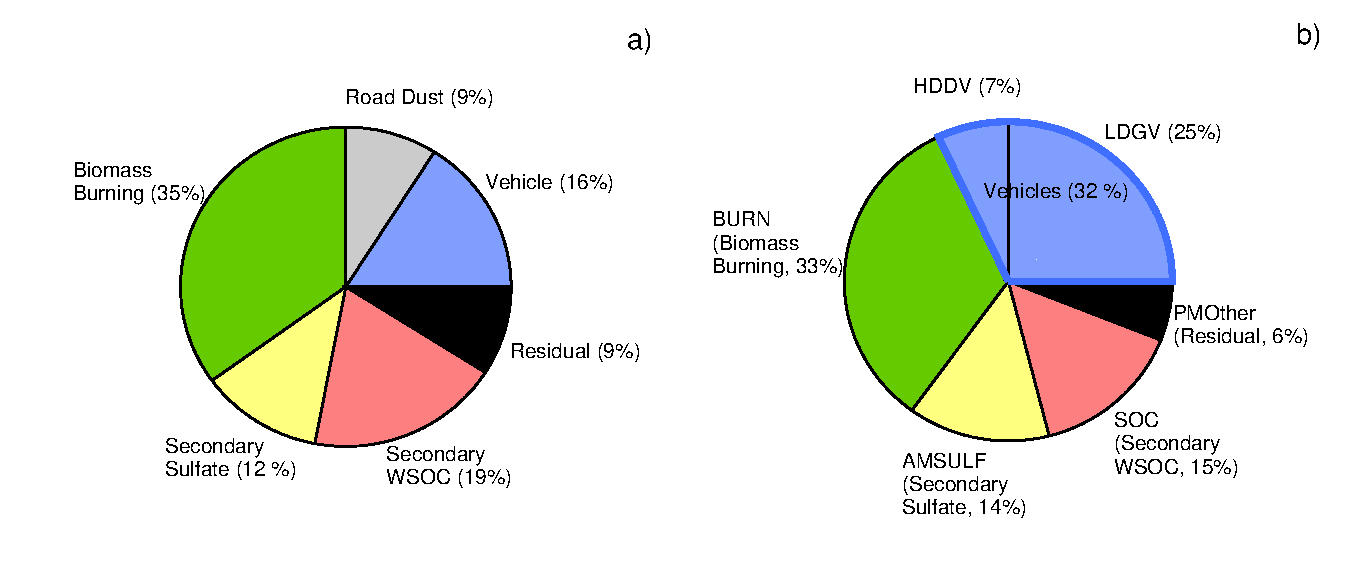
\includegraphics[width=1.0\linewidth]{figures/chapter04/verma_2014_fig8.pdf}
    \caption{Première estimation de la contribution des sources de PM au \PODTT{} par
        \cite[][figure 8]{vermaReactive2014}: \textbf{a)} par ajout du DTT dans la PMF et
        \textbf{b)} par régression linéaire entre \PODTT{} et CMB.
    }%
    \label{fig:figures/chapter04/verma_2014_fig8}
\end{figure}

Seulement, nous avons vu que les PMF sont très sensible aux variables utilisées. Or, leurs
études PMF inclut un ensemble d'espèce chimiques restreint (une dizaine de métaux et le
WSOC), en plus du PO. Seuls 4 facteurs sont identifiés par \cite{fangOxidative2016}, ce
qui semble peu au regard des PMF utilisant un jeu d'espèce chimique plus conséquente (voir
notamment tous le chapitre précédent). En plus, ce faible nombre d'espèces chimiques
associés à une nouvelle variable, le PO, dont nous ne connaissons a priori que peu de chose de ses
sources, peut conduire à des solutions instables statistiquement.

La solution utilisant la régression linéaire à partir du CMB hérite des limitations
propre au CMB : peu de prise en compte des particularités locales, connaissance a priori
forte, etc (voir section
~\ref{ssub:atouts_et_limitations_des_différents_modèles_récepteurs}).
Ainsi, \cite{batesSource2018} utilise un modèle CMB pour prédire à large échelle spatiale
(Amérique du Nord) le PO, mais le modèle établit présente de faible performance
statistique ($r^2 = 0.36$ et intercepte non nul), notamment du fait de l'oubli potentiel de
sources importantes (bioaérosols \autocite{samakeUnexpected2017}, etc).

\subsubsection{Couplage de PMF avancée avec l'estimation du PO}%
\label{sub:couplage_de_pmf_avancée_avec_l_estimation_du_po}

Je propose dans cette section de coupler les connaissances acquises sur les PMF présentées
dans le chapitre~\ref{cha:approfondissement_des_connaissances_des_sources_des_pm}
précédent, en n'ajoutant pas le PO comme variable explicative pour ne pas perturber le
modèle, puis d'évaluer le PO intrinsèque (i.e. par microgramme) de chacune des sources
identifiées, illustré par la figure~\ref{fig:workflow_inversion}.

Le site de Chamonix entre 2013 et 2014 a été choisi pour tester cette méthode du fait
d'une étude PMF approfondie par \cite{chevrierChauffage2016} et par les mesures de PO sur
ce site effectué lors de la thèse de \cite{calasPollution2017}, aussi bien pour le \POAA{}
que le \PODTT, et a fait l'objet d'une publication présenté ci-après.

\begin{figure}[ht]
    \centering
    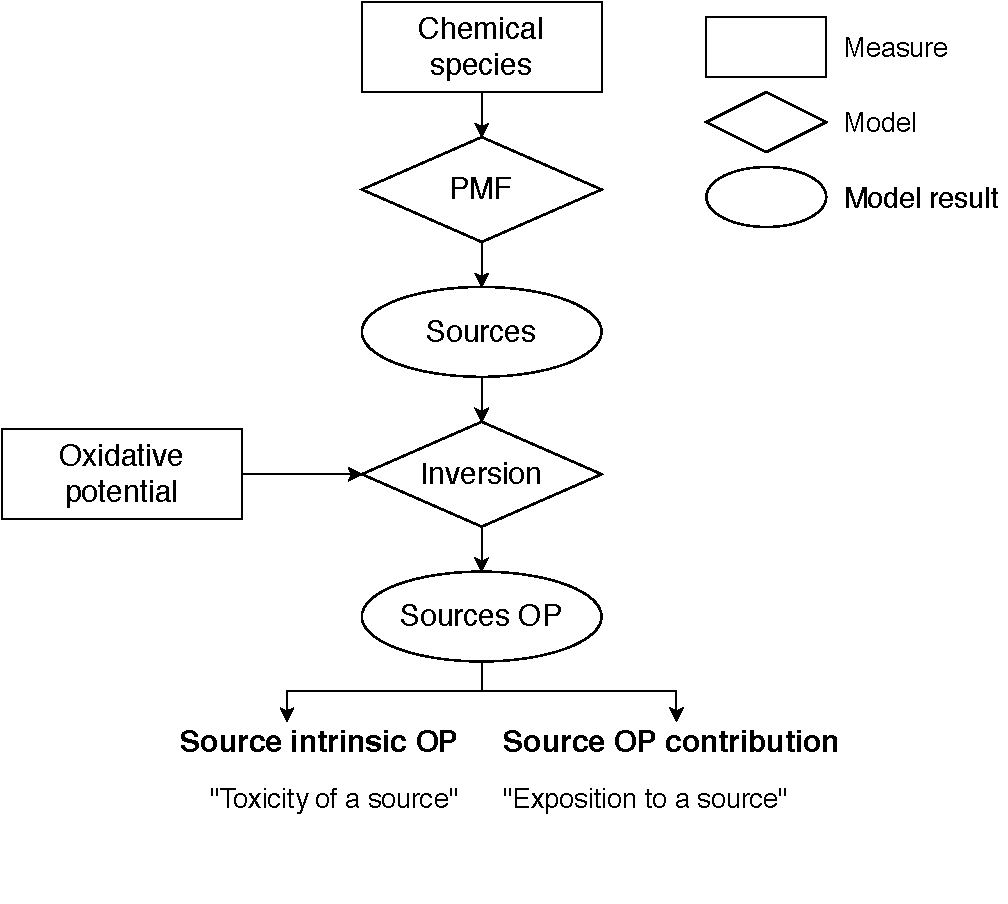
\includegraphics[width=0.8\linewidth]{figures/chapter04/flowchart_inversion.pdf}
    \caption{Processus suivi afin d'estimer la contribution des sources de PM aux
        potentiels oxydants. La méthode d'inversion utilisée dans ce chapitre est une
        régréssion linéaire multiple, permettant d'attribuer un PO par microgramme de source
        (\textit{PO intrinsèque}), estimant la ``toxicité de la source'', et la contribution de
    chacune des sources aux PO, estimant l'exposition de la population à cette source.}%
    \label{fig:workflow_inversion}
\end{figure}

\clearpage
\subsection{An apportionment method for the oxidative potential of atmospheric particulate
matter sources: application to a one-year study in Chamonix, France}
\label{sec:weber_et_al_2018}

Article paru dans le journal \textit{Atmospheric Chemistry and Physics} le 4 juin 2019 :

\begin{quote}
    Samuël Weber, Gaëlle Uzu, Aude Calas, Florie Chevrier, Jean-Luc Besombes,
    Aurélie Charron, Dalia Salameh, Irena Ježek, Griša Močnik, et Jean-Luc Jaffrezo. 2018.
    \textit{An Apportionment Method for the Oxidative Potential of Atmospheric Particulate
    Matter Sources: Application to a One-Year Study in Chamonix, France}. Atmospheric
    Chemistry and Physics 18(13), pp. 9617‑9629.
    \textsc{doi} : \href{https://doi.org/10.5194/acp-18-9617-2018}{10.5194/acp-18-9617-2018},
    \textsc{url} : \url{https://www.atmos-chem-phys.net/18/9617/2018/}
\end{quote}

Les profils PMF, la corrélation entre espèces chimiques et PO et sources et
PO à titre de comparaison avec les études antérieures, sont présentés en complément de
l'article, repris en annexe~\ref{annexe:deconvol_OP_SI}.

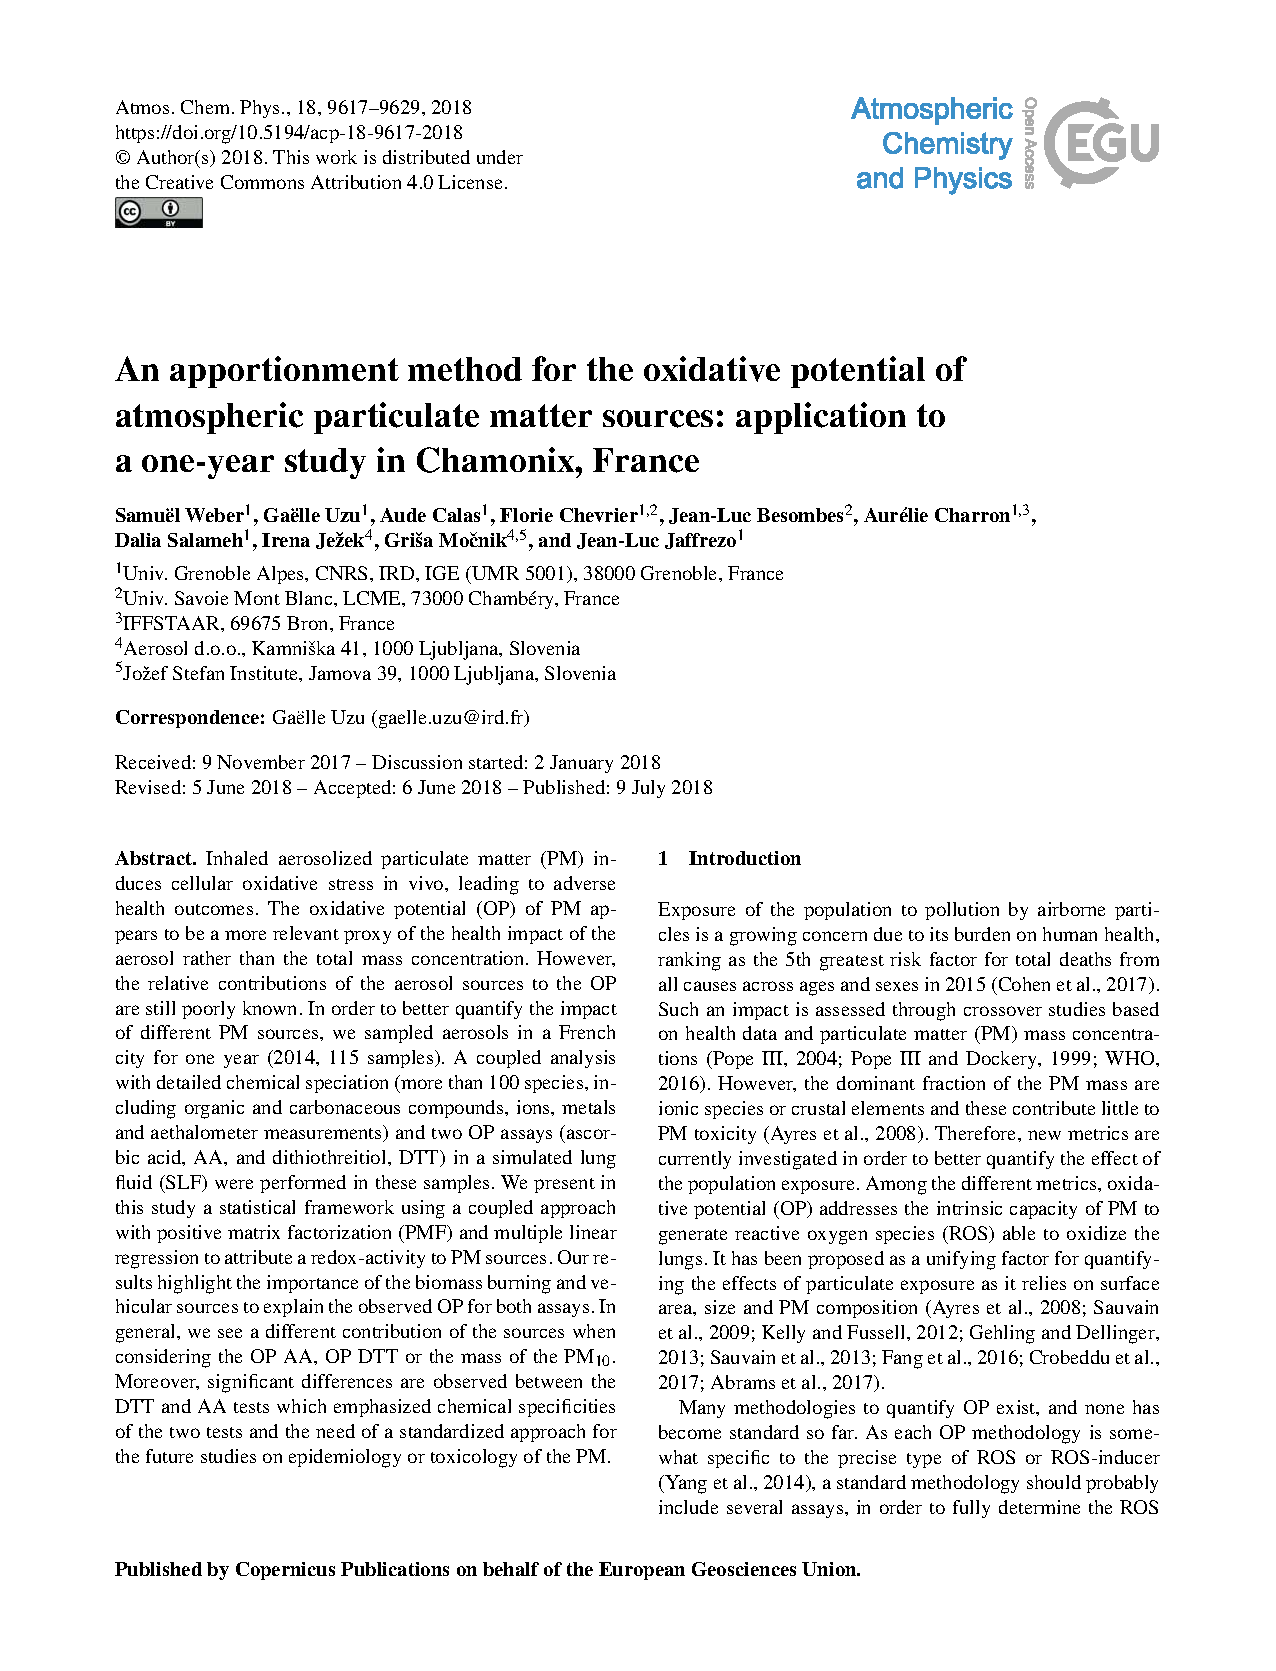
\includepdf[pages=-,scale=0.95,pagecommand={\pagestyle{fancy}}]{chapters/deconvol_OP.pdf}


\subsection{Conclusion}

Ce chapitre prouve tout d'abord qu'il est possible de déterminer les sources de PO grâce à
une étude couplée entre une PMF avancée utilisant différents traceurs organiques résultant
en 8 facteurs distincts et une régression linéaire multiple prenant en compte
la mesure du PO à iso-masse utilisant des conditions de bioaccessibilité proche du milieu
pulmonaire et ses incertitudes, avec une très bonne performance statistique.

Cette méthode permet de différencier très nettement les sources de PM contribuant aux PO
et apporte une vue nouvelle de l'aérosol en redistribuant l'importance de la contribution
des sources. Conformément aux résultats des 3 études précédentes faites aux États-Unis
\autocite{vermaReactive2014,batesReactive2015,fangOxidative2016}, la combustion de
biomasse domestique et le transport routier représentent les 2 sources principales de
\POAAv{} et \PODTTv.

L'utilisation de deux tests de PO nous permet aussi d'affirmer que ces 2 tests ne portent
pas en eux exactement les mêmes informations géochimiques, car les sources de PM les
expliquant diffèrent --bien que la même tendance générale est observée. En l'absence
d'étude approfondie quant aux liens toxicologie-PO ou épidémiologie-PO, le maintient de
différents tests de PO est donc recommandé.

Aussi, certaines corrélations observées, aussi bien avec des espèces chimiques que des
facteurs PMF, s'avère comme attendue trompeuse. Le facteur nitrate-rich était corrélé au
\POAAv{} mais présent en réalité un PO intrinsèque quasi-nul. Inversement, le facteur
secondaire biogénique, tracé par le MSA, est négativement corrélé aux deux \OPv{} alors
qu'il présente le 2\ieme{} \PODTT{} intrinsèque le plus élevé. Il est donc nécessaire
d'utiliser des méthodes statistiques plus avancées que la régression uni-variée lorsque
l'on cherche à estimer les sources de PO afin de s'affranchir des tendances sainonières et
des covariations entre espèces.

Cette méthode est donc validée comme outil de déconvolution des sources de PO, et le
prochain chapitre traitera de son application à un large panel d'environnement et année
d'étude, afin d'établir à la manière du chapitre précédent, une phénoménologie non pas des
sources de la masse \PMdix, mais des sources de PO.


\section{Synthèse grande échelle}%
\label{sec:synthèse_grande_échelle}

\subsection{Article}%
\label{sub:article}

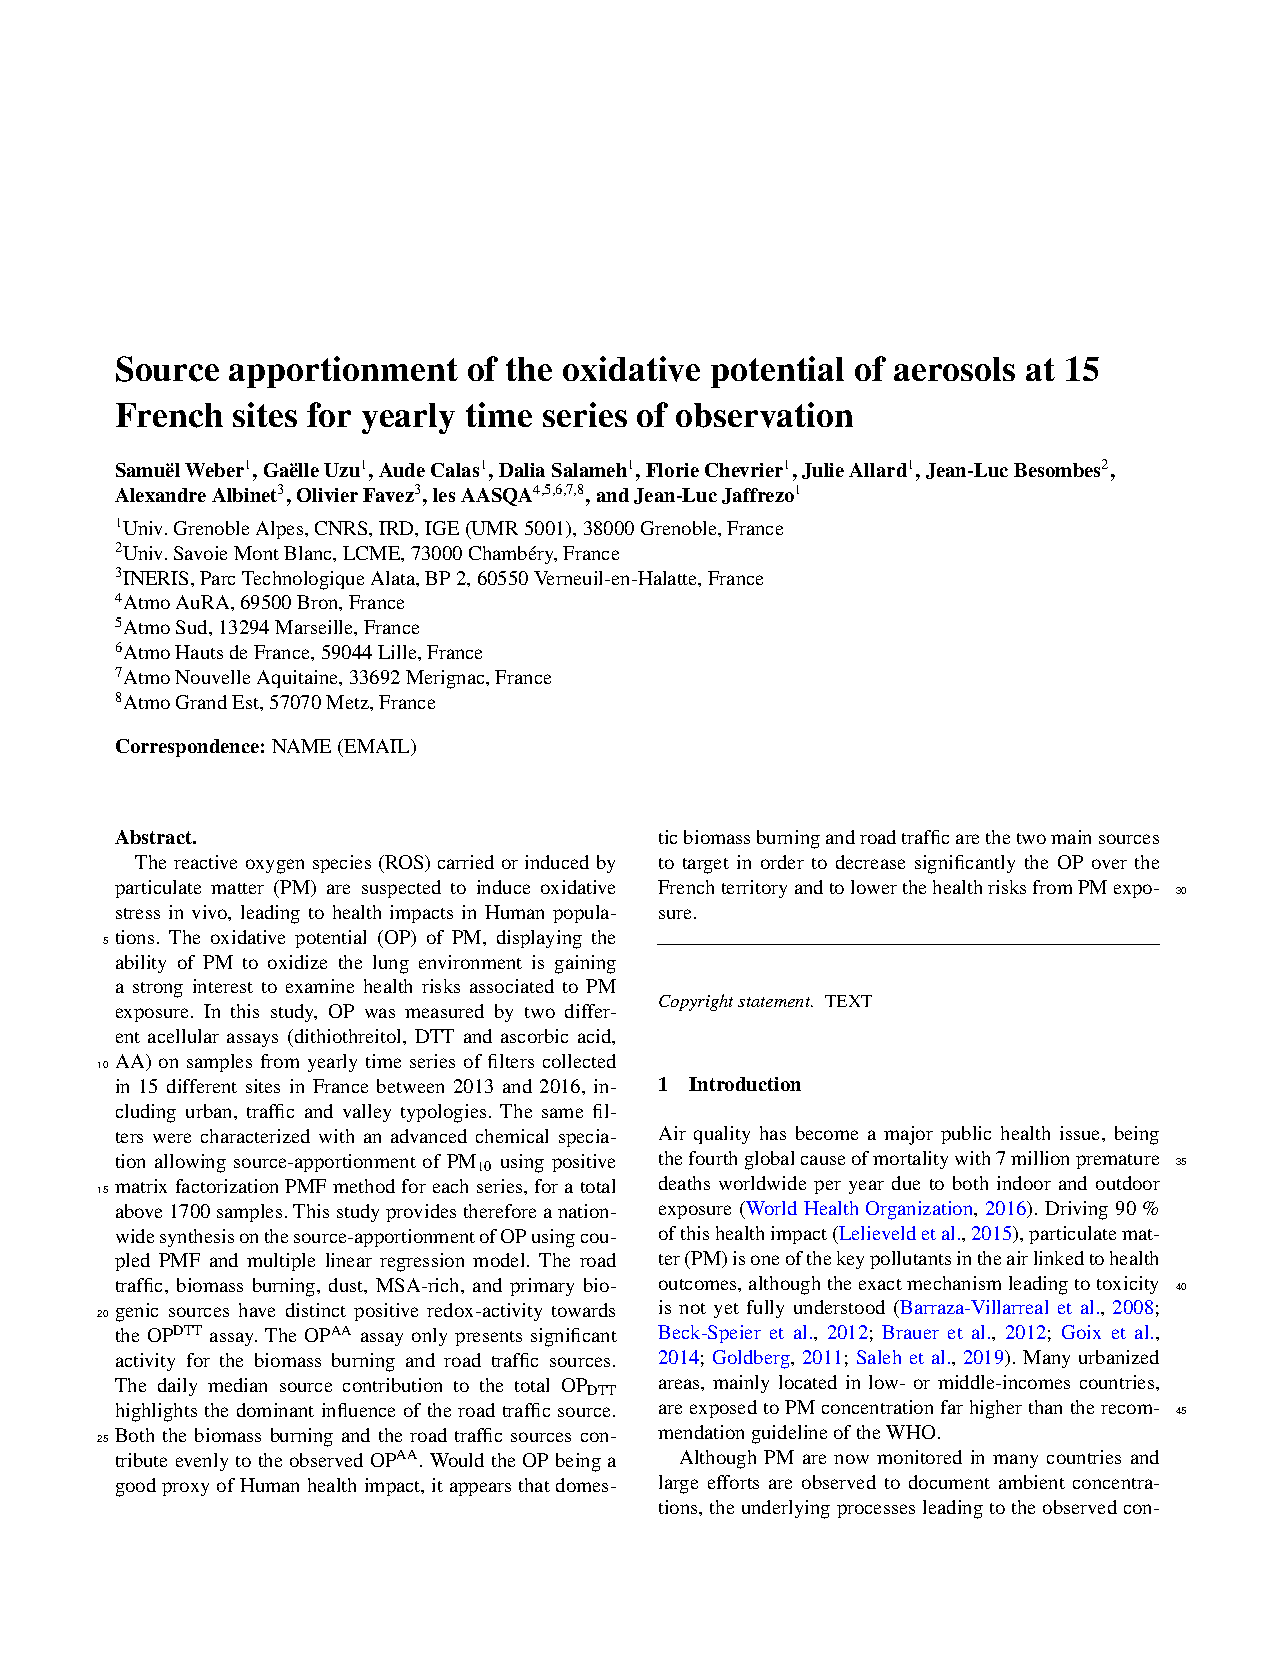
\includepdf[pages=-,scale=0.95,pagecommand={\pagestyle{fancy}}]{chapters/article_allOP/article_nuage.pdf}


\chapter{Passage à l'échelle régionale : application à 15 sites d'étude en France}
\label{cha:application_to_15_sites_in_France}
\PartialToc
\clearpage
% \input{chapters/chapter05_synthese_PO.tex}

\chapter{Vers une modélisation spatialisé du PO}
\label{cha:spatio_temporal_modelizing}
\PartialToc
\clearpage
% \input{chapters/chapter06_spatialisation.tex}

% =====================================================================================
% Bibliographie complète {{{
% \addcontentsline{toc}{part}{Bibliography}
% \printbibheading
\printbibliography
% \bibbysegment[heading=subbibliography]

% }}}
% =====================================================================================

% =====================================================================================
% Appendix {{{
\addcontentsline{toc}{part}{Appendix}
\appendix
\setcounter{table}{0}
\setcounter{figure}{0}
\setcounter{equation}{0}
\renewcommand{\thetable}{\thesection-\arabic{table}}
\renewcommand{\thefigure}{\thesection-\arabic{figure}}
\renewcommand{\theequation}{\thesection-\arabic{equation}}
% }}}
% =====================================================================================
\end{document}
